% chapter: 実際の解き方

\chapter{実際の解き方}\label{章：実際の解き方}
\begin{bookcolumns}

  差を取る、倍率をそろえる、複数の項をまとめる。
  これまでの操作を、式の特徴と結び付けて見直す。
  一つの問題に複数の方法が使えるときは、その条件と残る計算を比べる。
% section: 解法の決定

\section{解法の決定}\label{節：解法の決定}
  以下にここまでで扱った解法を体系的にまとめあげ,実際に問題と相対した時にどこに注目すればよいか,なにを考えればよいかをまとめた.
  \chapterref{章：漸化式の解説}で目指してきたように,式の特徴を手掛かりとして,既知の「きれい」な形に帰着させることを考えよう.

  チャートは「式全体」「数列の項」「足されている数」の3つの観点から,着目点と試せる変形を整理したものである.
  すべてを順番に確認する必要はなく,式の中で目立つ特徴から必要な項目を使えばよい.
  一つの式に複数の特徴が当てはまることもある.どの特徴を使い,どの順番で変形するかは,この後の問題演習で練習していこう.
  変形した後にも,新しい式について同じ着目点を確認するとよい.

  \noindent\textbf{【観察から変形まで】}\par
  次の4段階を,必要に応じて繰り返す.チャートの出口は候補であり,一つの正解に固定するものではない.
  \begin{enumerate}
    \item \textbf{観察}：総和,分母,倍率,付加項のうち,何が目立つかを具体的な式で指す.
    \item \textbf{候補}：その特徴が変形後に消えるか,一定になるかを考える.複数の候補があってよい.
    \item \textbf{条件}：割る量の非零,対数の真数の正値,初項による定数解の分岐を確かめる.
    \item \textbf{変形と評価}：新しい量の更新を一行計算し,何が簡単になったかを見る.新しい式を観察し直し,必要なら別の候補へ戻る.
  \end{enumerate}
  候補が正しくても計算が長くなる場合はある.条件の見やすさと計算量も比較しよう.
  一般項が得られたら,初期条件と元の更新式を確認する.

  \begingroup
  \clubpenalty=10000
  \widowpenalty=10000
  \medskip
  \noindent \textbf{【チャート1：式全体について】}
  \begin{enumerate}
    \item \textbf{総和$S_n$があるか}

      $S_n=\sum_{k=1}^{n}a_k$なら,\,$S_{n+1}-S_n=a_{n+1}$である.
      添字を一つずらした式との差を取り,総和を消去できないか考える（総和型）.

    \item \textbf{数列の項を含む式が分母にあるか}

      逆数を取って簡単にならないか考える.
      定数係数の1次式同士の商なら,定数を引いて逆数型へ帰着させる方法もある（分数型）.
      分母が$0$にならないことを確認する.

    \item \textbf{何項間か.添字は隣接しているか}

      例えば$a_{n+2}$と$a_n$の関係なら,奇数番目と偶数番目を別々の数列として考えられる（非隣接2項間漸化式型）.
      また,\,$a_{n+2}=qa_n$は
      \[
        a_{n+2}=0\cdot a_{n+1}+qa_n
      \]
      と書ける.定数係数で,各項が1次の和として現れるなら,欠けた項を係数$0$で補い,隣接3項間・4項間の解法を検討する.

    \item \textbf{展開・因数分解・通分で簡単になるか}

      見た目が複雑でも,整理すると基本的な形が現れることがある.
      分数を約分する際には,消す因子が$0$になる場合を別に確認する.

    \item \textbf{同じ式のまとまりが繰り返し現れるか}

      例えば$a_n+n$と$a_{n+1}+(n+1)$が現れるなら,\,$b_n=a_n+n$と置いて関係を調べる.

    \item \textbf{既知の公式に似ているか}

      $a_n^2-2$のような形なら,積が$1$となる二つの数の和を使う置換を考える（基本対称式型）.
      $2a_n^2-1$や$\displaystyle \frac{2a_n}{1-a_n^2}$は,三角関数の倍角公式を思い出す手掛かりになる（三角関数型）.
      $\displaystyle \frac12\left(a_n+\frac{c}{a_n}\right)$のような平均の形なら,ニュートン法型を検討する.
      見た目に加えて,初項や置換の条件も確認する.

    \begin{samepage}
    \item \textbf{複数の数列の関係が与えられているか}\\*[3pt]
      定数係数の線形連立漸化式なら,数列の和・差などを使って一つずつの関係に分けられないか考える（連立型）.
    \par
    \end{samepage}

    \item \textbf{整数部分を表す記号があるか}

      まず,整数部分の記号が項の値・添字・付加項のどこに作用しているかを見る（ガウス型）.
      項の値なら整数性や余り,添字なら偶奇や群への分割,付加項なら同じ値を取る範囲が手掛かりになる.
      床関数を外せるかを調べるときは,整数性と上下の不等式を確かめる.
  \end{enumerate}

  \medskip
  \noindent \textbf{【チャート2：数列の項について】}

  係数については,主に$a_{n+1}=p_na_n+f(n)$の形に整理できる場合を考える.
  \begin{enumerate}
    \item \textbf{係数は定数か,\,$n$に依存するか}

      \begin{itemize}[beginpenalty=10000]
        \item 定数の場合は,等比型や特性方程式型などを考える.係数が$1$なら,階差に注目する.
        \item $n$に依存する場合は,その係数の積が求めやすいか調べる（階比型）.
              足されている数もある場合は,適切な数列で割って係数をそろえられないか考える.
              例えば係数が$\displaystyle \frac{n+1}{n}$なら,\,$b_n=\displaystyle \frac{a_n}{n}$という置換が候補になる.
      \end{itemize}
      係数だけで判断せず,足されている数についてもチャート3を確認する.

    \item \textbf{累乗の指数はどうなっているか}

      \begin{itemize}[beginpenalty=10000]
        \item すべて1次か.2次以上なら,因数分解や$a_n^2$などのまとまりを使う置換を考える.
        \item 指数は定数か,\,$n$に依存するか.対数を取ると,指数を係数として取り出せる場合がある（対数型）.
      \end{itemize}
      実数の対数を取る各量は,正であることを確認する.

    \item \textbf{数列の項同士の積や商があるか}

      $a_na_{n+1}$などの積があるなら,因数分解や置換でまとまりを作れないか考える.
      積・商・累乗を対数で和・差・定数倍に変えられるかも調べる.
      ただし,和の対数を各項の対数の和に分けることはできない.
  \end{enumerate}

  \medskip
  \noindent \textbf{【チャート3：足されている数について】}

  ここでは,数列の項を含まずに足されている部分を「付加項」と呼ぶ.
  以下では$a_{n+1}=p_na_n+f(n)$の形を考え,\,$f(n)$を調べよう.
  \begin{enumerate}
    \item \textbf{付加項はないか,定数か}

      付加項がなければ,係数の積から求める方法を考える（等比型・階比型）.
      付加項も係数も定数なら,定数を引いて消せないか考える（特性方程式型）.
      ただし$a_{n+1}=a_n+d$なら,そのまま等差型として解ける.

    \item \textbf{$n$に依存するなら,どのような形か}

      \begin{itemize}[beginpenalty=10000]
        \item \textbf{指数の形}：$cq^n$などなら,\,$q\ne0$を確認し,\,$q^n$などで割って指数の部分を取り除くことを考える.
        \item \textbf{$n$の多項式}：$n^2+2n$などで係数が定数なら,多項式を引いて付加項を消す方法を考える（階差等比複合型）.
        \item \textbf{多項式と指数の積}：$n2^n$などなら,まず指数の部分で割り,残った多項式をどう扱うか考える.
      \end{itemize}
      例えば$n+2^n$のように複数の形が混ざっていれば,それぞれの部分を見る.

    \item \textbf{総和を求めやすい形にできるか}

      階差型へ帰着できたら,付加項の総和を考える.
      $n(n+1)$のような連続整数の積や,隣り合う項の差として表せないか調べる.
      差の形にできれば,総和を取ったときに途中の項が消える.
  \end{enumerate}

  \medskip
  \noindent \textbf{【補足：初項も手掛かりになる】}

  例えば初項が$\displaystyle \frac{1}{\sqrt{6}-\sqrt{2}}$だとしよう.
  わざわざこのような数字が設定されたということはきっと裏がある.
  実際これは$\cos 15^\circ$または$\sin 75^\circ$の値である.
  そこから考えて,この漸化式は三角関数型のものではないか,と予想するのである.
  ただし,初項だけで解法が決まるわけではない.漸化式の形と合わせて判断しよう.
  \par
  \endgroup

% 解法の選択を、計算の前に確認する短い練習。
\subsection{操作を選ぶ練習}\label{節：操作を選ぶ練習}
  ここでは\bookterm{general}{一般項}まで一気に計算する前に,新しい量を選び,その更新だけを確かめる.
  引く・割る・\bookterm{logarithm}{対数}を取るという操作が,それぞれ何を簡単にするかを比較しよう.

  \noindent\bookblocklink{operation-choice}{problem}{answer}{【問題】}\par\nobreak
  \begin{enumerate}[format=\bookitemlink{operation-choice}{problem}{answer}]
    \item $a_1=1$,\,$a_{n+1}=3a_n+2n+1$とする.
          定数を引くだけで付加項を消せるか.
          $g(n)=un+v$を引く場合の$u,v$を求め,\,$b_n=a_n-g(n)$の更新式と初項を示せ.
    \item $a_1=2$,\,$a_{n+1}=\frac{n+2}{n}a_n+(n+1)(n+2)$とする.
          $b_n=\frac{a_n}{n}$と$c_n=\frac{a_n}{n(n+1)}$を候補とし,それぞれの更新式を求めよ.
          どちらで$a_n$の係数を$1$にそろえられるか.
    \item $a_1=-2$,\,$a_{n+1}=2^{2n+1}a_n$とする.
          $b_n=\log_2a_n$は使えるか.
          \bookterm{logarithm}{対数}を使わず,\,$c_n=\frac{a_n}{2^{n^2}}$の更新式と初項を求めよ.
  \end{enumerate}

  第2問は,\sectionref*{節：階比型}で倍率をそろえた操作を,付加項がある場合に使う練習である.
  一般に
  \[
    a_{n+1}=p_na_n+q_n
  \]
  に対して,既知の非零の\bookterm{sequence}{数列}$h_n$が$h_{n+1}=p_nh_n$を満たすなら,
  \[
    b_n=\frac{a_n}{h_n},\qquad
    b_{n+1}-b_n=\frac{q_n}{h_{n+1}}
  \]
  となる.倍率をそろえる操作の後に,\bookterm{difference}{階差}を足し戻す操作が続く.
  $p_n\ne0$なら,\,$h_1=1$,\,$h_n=\prod_{k=1}^{n-1}p_k$を候補にできる（空積は$1$）.
  係数が零になる場合はこの割り算を使わず,その段階の更新を別に確認する.
  また,残った和がいつでも簡単に計算できるとは限らない.

  \noindent\bookblocklink{operation-choice}{answer}{problem}{【解答と選択の理由】}\par\nobreak
  \begin{enumerate}[format=\bookitemlink{operation-choice}{answer}{problem}]
    \item $a_n-\alpha$では付加項の$2n$が残る.
          $g(n+1)=3g(n)+2n+1$から
          \[
            u=3u+2,\qquad u+v=3v+1
          \]
          となり,\,$u=v=-1$である.
          従って$b_n=a_n+n+1$により$b_{n+1}=3b_n$,\,$b_1=3$を得る.
          引く量を定数から一次式へ変えたことで,付加項を消せた.

    \item 候補ごとに一歩だけ更新すると,
          \[
            b_{n+1}=\frac{n+2}{n+1}b_n+n+2
          \]
          と
          \[
            c_{n+1}=c_n+1,\qquad c_1=1
          \]
          を得る.
          $h_n=n(n+1)$なら
          \[
            \frac{h_{n+1}}{h_n}=\frac{n+2}{n}
          \]
          が元の倍率と一致する.
          この一致を手掛かりに割る因子を選ぶ.
          $n\ge1$なので分母は非零であり,\,$c_n=n$から$a_n=n^2(n+1)$も得られる.

    \item 正の倍率で更新するので,各項は負であり,\,$\log_2a_n$は実数として定義できない.
          一方,\,$2n+1=(n+1)^2-n^2$から
          \[
            c_{n+1}=c_n,\qquad c_1=-1
          \]
          となる.従って$a_n=-2^{n^2}$を得る.
          \bookterm{normalize}{正規化}で割る$2^{n^2}$は常に非零であり,元の項が正である必要はない.
          初項が正の比較例は\bookproblemref{practice-basic}{42}{標準問42}へ.
  \end{enumerate}


 \section{解法の変更}\label{節：解法の変更}

  先に挙げた着目点から試した変形でも簡単にならない時は,一度最初からやり直してみるとよい.
  この際に今までと同じ考え方ではなく,なるべく別のアプローチができないか検討すると解法を見つけやすい.

  また,それ以外の場合でも次のどれかが起こったら,今の方法を一度止め,解法の再検討を行うと良い.
  \begin{enumerate}
    \item 対数を取っても,数列の項を1次の和として表せない.
    \item 定数を引いて付加項を消そうとしたが,条件を満たす定数が求まらない.
    \item 置換後に新しい種類の項が増え続ける.
  \end{enumerate}
  このようなときには$a_2$から$a_5$ぐらいまでの値を求めてみると法則性に気づき,帰納法で証明できる場合がある.
  

  それでも見つけられない時は,特殊関数型の置換や,まだ試していない式変形も候補に入れよう.
  一旦ご飯でも食べて改めて取り組もう.
  ご飯の時間でないのなら,今までの数学の知識を総動員して似たものを探そう.
  
  \begin{samepage}
  この手順を身につけると,個別のパターンを暗記するだけでなく,
  見慣れない漸化式にも最初の一手を選べるようになる.
  \par
  \end{samepage}


\section{計算と検算の確認}\label{節：読む前の確認}
ここまでに使った、添字・和・式変形・検算を確かめる五題である。
解答には、計算の理由を読み返す場所も示した。

    \noindent\bookblocklink{reading-check}{problem}{answer}{【確認問題】}\par\nobreak
    \begin{enumerate}[format=\bookitemlink{reading-check}{problem}{answer}]
      \item $a_{n+1}=2a_n+n$の添字$n$を$n+1$に置き換えた式を書け.
      \item $\displaystyle\frac1{x(x+1)}=\frac1x-\frac1{x+1}$を確かめ,使える$x$の範囲を述べよ.
      \item $\displaystyle\sum_{k=1}^{3}k$と$\displaystyle\sum_{k=1}^{3}2^{k-1}$を計算せよ.
      \item $b_n=a_n+3$,\,$b_1=4$,\,$b_{n+1}=2b_n$から$a_n$を求めよ.
      \item $a_1=1$,\,$a_{n+1}=a_n+2$について,最初の3項が$1,3,5$であることだけで$a_n=2n-1$を証明できるか.すべての項で示すために何を確かめるか.
    \end{enumerate}

    \noindent\bookblocklink{reading-check}{answer}{problem}{【解答と戻り先】}\par\nobreak
    \begin{enumerate}[format=\bookitemlink{reading-check}{answer}{problem}]
      \item $a_{n+2}=2a_{n+1}+n+1$.
            項と付加項の添字を両方ずらす.\sectionref*{節：シグマの計算}では添字の役割を確認する.
      \item 通分すると右辺は$\displaystyle\frac{(x+1)-x}{x(x+1)}$となる.
            $x\ne0,-1$が必要である.\sectionref*{節：式の変形}へ.
      \item $6$と$7$.
            \sectionref*{節：シグマの計算},\sectionref*{節：等差数列とその総和の導出},\sectionref*{節：等比数列の総和とその導出}へ.
      \item $b_n=4\cdot2^{n-1}$より$a_n=4\cdot2^{n-1}-3$.
            元へ戻す際は$a_n=b_n-3$である.\sectionref*{節：等比型}へ.
      \item 3項の一致は予想の手掛かりである.
            初項の一致と,任意の$n\ge1$について$a_n=2n-1$なら$a_{n+1}=2(n+1)-1$となることを確かめる.
            \sectionref*{節：数学的帰納法}へ.
    \end{enumerate}


% 問題演習を第4章の節として読み込む。
% chapter: 問題演習

  \section{問題演習}\label{節：問題演習}
    ここでは,これまでに扱った漸化式の解法を実際の問題を通して確認する.
    標準難易度55題では,基本・応用11パターンを横断し,式の構造から解法を選ぶ.
    応用難易度10題では,複数の解法をどの順番で組み合わせるかを考える.
    発展難易度10題では,漸化式を立てて,さまざまな数学の対象を調べる.
    方針・解答・解法は問題と同じ問番号に対応し,問番号から対応箇所へ移動できる.

% 第4章 標準難易度：基本4パターン・応用7パターンを各5題。
% 主分類・出題意図・別解の対応は docs/chapter4-standard-design-2026-10-04.md。

    \subsection{標準難易度}\label{節：標準難易度}\label{節：基本と応用から出題されるもの}
      ここでは,第3章の基本4パターンと応用7パターンから,それぞれ5題ずつ,計55題を出題する.
      同じ解法で解ける問題も,式の並び方や係数が変わると違って見える.
      まず移項や約分によって式を整理し,どの数量の差や比に注目すればよいかを考えよう.
      問題は型ごとにまとめずに並べてあるので,式の構造を見て解法を選んでほしい.
      方針と解法は問題と同じ問番号に対応する.
      別解のある問題では,最初の解法を理解したあとに,別の見方でも同じ答えになることを確認しよう.
      特に階比型と対数型には共通して使える見方がある.
      以下,\,$n$は正の整数とし,必要なときは
      \[
        S_n=\sum_{k=1}^{n}a_k
      \]
      とおく.

      \subsubsection{問題}\label{節：標準難易度：問題}\label{節：基本と応用から出題されるもの：問題}
        \begin{enumerate}[label=\textbf{問\arabic*.},leftmargin=3.8em,format=\bookitemlink{practice-basic}{problem}{answer}]
          % Q1
          \item $\displaystyle a_1=3$ とし,
                \[
                  (2a_n+3)a_{n+1}=3a_n
                \]
                を満たす数列$\{a_n\}$の一般項を求めよ.
          % S1
          \item $\displaystyle S_n=2a_n-n^2$
                                を満たす数列$\{a_n\}$の一般項を求めよ.
          % R1
          \item $\displaystyle a_1=3,\qquad a_{n+1}=2(n+1)a_n$
                で定められる数列の一般項を求めよ.
          % M1
          \item $\displaystyle a_1=2,\qquad a_{n+1}=2a_n+n-1$
                で定められる数列$\{a_n\}$の一般項を求めよ.
          % G1
          \item $\displaystyle a_1=6,\qquad a_{n+1}=-\frac12a_n$
                で定められる数列の一般項を求めよ.
          % T1
          \item $\displaystyle a_1=2,\,a_2=5$ とし,
                \[
                  a_{n+2}+6a_n=5a_{n+1}
                \]
                を満たす数列$\{a_n\}$の一般項を求めよ.
          % U1
          \item $\displaystyle a_1=3,\qquad b_1=1,$
                            \[
                              \begin{cases}
                                a_{n+1}=2a_n-b_n,\\
                                b_{n+1}=-a_n+2b_n
                              \end{cases}
                            \]
                                で定められる2つの数列$\{a_n\},\{b_n\}$の一般項を求めよ.
          % L1
          \item $\displaystyle a_1=4,\qquad a_{n+1}=\frac{a_n^3}{4}$
                で定められる数列$\{a_n\}$の一般項を求めよ.
          % C1
          \item $\displaystyle a_1=5,\qquad a_{n+1}=3a_n-4$
                で定められる数列$\{a_n\}$の一般項を求めよ.
          % D1
          \item $\displaystyle a_1=\frac56,\qquad 3a_{n+1}=3a_n-2$
                で定められる数列の一般項を求めよ.
          % F1
          \item $\displaystyle a_1=2,\qquad a_{n+1}=a_n+3n-1$
                で定められる数列の一般項を求めよ.
          % T2
          \item $\displaystyle a_1=3,\,a_2=1$ とし,
                \[
                  a_{n+2}+a_{n+1}=6a_n
                \]
                を満たす数列$\{a_n\}$の一般項を求めよ.
          % F2
          \item $\displaystyle a_1=1,\qquad a_{n+1}=a_n+3n^2+3n+1$
                で定められる数列の一般項を求めよ.
          % Q2
          \item $\displaystyle a_1=2,\,a_{n+1}=-\frac{2a_n}{3a_n+2}$
                で定められる数列$\{a_n\}$の一般項を求めよ.
          % C2
          \item $\displaystyle a_1=1,\qquad 2a_{n+1}+a_n=9$
                で定められる数列$\{a_n\}$の一般項を求めよ.
          % U2
          \item $\displaystyle a_1=3,\qquad b_1=1,$
                            \[
                              \begin{cases}
                                a_{n+1}=4a_n-2b_n,\\
                                b_{n+1}=a_n+b_n
                              \end{cases}
                            \]
                                で定められる2つの数列$\{a_n\},\{b_n\}$の一般項を求めよ.
          % D2
          \item $\displaystyle a_1=-4,\qquad 2a_{n+1}+a_n=3a_n+6$
                で定められる数列の一般項を求めよ.
          % G2
          \item $\displaystyle a_1=3,\qquad 2a_{n+1}-5a_n=a_{n+1}+a_n$
                で定められる数列の一般項を求めよ.
          % R2
          \item $\displaystyle a_1=6,\qquad
                 (n+1)(n+2)a_{n+1}=n(n+3)a_n$
                で定められる数列の一般項を求めよ.
          % M2
          \item $\displaystyle a_1=3,\qquad a_{n+1}+a_n=2n^2+2n+1$
                で定められる数列$\{a_n\}$の一般項を求めよ.
          % S2
          \item $\displaystyle S_n=a_n+(n-1)2^{n-1}$
                                を満たす数列$\{a_n\}$の一般項を求めよ.
          % L2
          \item $\displaystyle a_1=5,\qquad a_{n+1}=a_n^2-4a_n+6$
                で定められる数列$\{a_n\}$の一般項を求めよ.
          % T3
          \item $\displaystyle a_1=1,\,a_2=0$ とし,
                \[
                  a_{n+2}-4a_{n+1}+4a_n=0
                \]
                を満たす数列$\{a_n\}$の一般項を求めよ.
          % M3
          \item $\displaystyle a_1=1,\qquad a_{n+1}=3a_n-2^n$
                で定められる数列$\{a_n\}$の一般項を求めよ.
          % U3
          \item $\displaystyle a_1=1,\qquad b_1=2,$
                            \[
                              \begin{cases}
                                a_{n+1}=2a_n+b_n,\\
                                b_{n+1}=2b_n
                              \end{cases}
                            \]
                                で定められる2つの数列$\{a_n\},\{b_n\}$の一般項を求めよ.
          % Q3
          \item $\displaystyle a_1=4,\,a_{n+1}=\frac{3a_n+2}{a_n+2}$
                で定められる数列$\{a_n\}$の一般項を求めよ.
          % G3
          \item $\displaystyle a_1=4,\qquad (n+1)a_{n+1}=\frac{n+1}{3}a_n$
                で定められる数列の一般項を求めよ.
          % D3
          \item $\displaystyle a_1=1-\sqrt2,\qquad a_{n+1}+n=a_n+n+\sqrt2$
                で定められる数列の一般項を求めよ.
          % L3
          \item $\displaystyle a_1=2,\qquad a_{n+1}=a_n^{\frac{n+2}{n}}$
                で定められる正の数列$\{a_n\}$の一般項を求めよ.
          % S3
          \item $\displaystyle S_1=1,\qquad S_{n+1}=3S_n+2$
                                を満たす数列$\{a_n\}$の一般項を求めよ.
          % F3
          \item $\displaystyle a_1=3,\qquad a_{n+1}=a_n+2\cdot3^n$
                で定められる数列の一般項を求めよ.
          % R3
          \item $\displaystyle a_1=4,\qquad (n+1)^2a_{n+1}=n^2a_n$
                で定められる数列の一般項を求めよ.
          % C3
          \item $\displaystyle a_1=0,\qquad a_{n+1}-a_n=\frac{6-a_n}{3}$
                で定められる数列$\{a_n\}$の一般項を求めよ.
          % S4
          \item $\displaystyle a_1=1,\qquad a_{n+1}=2S_n+2^n$
                                で定められる数列$\{a_n\}$の一般項を求めよ.
          % Q4
          \item $\displaystyle a_1=1,\,a_{n+1}=2+\frac3{a_n}$
                で定められる数列$\{a_n\}$の一般項を求めよ.
          % G4
          \item 数列$\{a_n\}$は,ある実数$r$について
                \[
                  a_{n+1}=ra_n
                \]
                を満たし,\,$a_2=-6$,\, $a_5=48$である.\,$r$および一般項$a_n$を求めよ.
          % F4
          \item $\displaystyle a_1=0,\qquad a_{n+1}=a_n+\frac{2}{(n+1)(n+3)}$
                で定められる数列の一般項を求めよ.
          % T4
          \item $\displaystyle a_1=3,\,a_2=5$ とし,
                \[
                  a_{n+2}=2a_{n+1}+3a_n-8
                \]
                を満たす数列$\{a_n\}$の一般項を求めよ.
          % U4
          \item $\displaystyle a_1=0,\qquad b_1=1,$
                            \[
                              \begin{cases}
                                a_{n+1}=2a_n+b_n+1,\\
                                b_{n+1}=a_n+2b_n-1
                              \end{cases}
                            \]
                                で定められる2つの数列$\{a_n\},\{b_n\}$の一般項を求めよ.
          % L4
          \item $\displaystyle a_1=1,\qquad a_{n+1}=2\sqrt{a_n}$
                で定められる数列$\{a_n\}$の一般項を求めよ.
          % C4
          \item 実数$t$に対し,
                \[
                  a_1=t,\qquad a_{n+1}=4a_n-9
                \]
                で数列$\{a_n\}$を定める.一般項を求め,この数列が定数数列となる$t$の値を求めよ.
          % R4
          \item $\displaystyle a_1=2,\qquad a_{n+1}=2^{2n+1}a_n$
                で定められる数列の一般項を求めよ.
          % D4
          \item 数列$\{a_n\}$は,ある実数$d$について
                \[
                  a_{n+1}=a_n+d
                \]
                を満たし,\,$a_3=8$,\, $a_8=-7$である.\,$d$,\, $a_1$および一般項$a_n$を求めよ.
          % M4
          \item $\displaystyle a_1=2,\qquad a_{n+1}=2a_n+3\cdot2^n$
                で定められる数列$\{a_n\}$の一般項を求めよ.
          % U5
          \item $\displaystyle a_1=1,\qquad b_1=0,$
                            \[
                              \begin{cases}
                                a_{n+1}=a_n+2b_n,\\
                                b_{n+1}=a_n
                              \end{cases}
                            \]
                                で定められる2つの数列$\{a_n\},\{b_n\}$の一般項を求めよ.
          % R5
          \item $\displaystyle a_1=1,\qquad a_{n+1}=\frac{n(n+1)}2a_n$
                で定められる数列の一般項を求めよ.
          % Q5
          \item $\displaystyle a_1=2,\,a_{n+1}=2-\frac1{a_n}$
                で定められる数列$\{a_n\}$の一般項を求めよ.
          % G5
          \item $\displaystyle a_1=0,\qquad a_{n+1}=7a_n$
                で定められる数列の一般項を求めよ.
          % L5
          \item $\displaystyle a_1=4,\qquad a_{n+1}=\frac{a_n^2}{2^{n-1}}$
                で定められる数列$\{a_n\}$の一般項を求めよ.
          % F5
          \item $\displaystyle a_1=1,\qquad a_{n+1}=a_n+(-1)^n$
                で定められる数列の一般項を求めよ.
          % C5
          \item 実数$p,q$を用いて,
                \[
                  a_{n+1}=pa_n+q
                \]
                で定められる数列$\{a_n\}$について,
                \[
                  a_1=8,\qquad a_2=5,\qquad a_3=\frac72
                \]
                であることが分かっている.\,$p,q$の値と一般項を求めよ.
          % T5
          \item $\displaystyle a_1=1,\,a_2=2$ とし,
                \[
                  a_{n+2}-3a_{n+1}+2a_n=1
                \]
                を満たす数列$\{a_n\}$の一般項を求めよ.
          % D5
          \item $\displaystyle a_1=\frac74,\qquad 4a_{n+1}-4a_n=0$
                で定められる数列の一般項を求めよ.
          % M5
          \item $\displaystyle a_1=0,\qquad a_{n+1}=2a_n+3(-1)^n$
                で定められる数列$\{a_n\}$の一般項を求めよ.
          % S5
          \item $\displaystyle a_1=2,\qquad S_n=\frac{n+2}{3}a_n$
                                を満たす数列$\{a_n\}$の一般項を求めよ.
        \end{enumerate}

      \subsubsection{方針}\label{節：標準難易度：方針}\label{節：基本と応用から出題されるもの：方針}
        \begin{enumerate}[label=\textbf{問\arabic*.},leftmargin=3.8em,format=\bookitemlink{practice-basic}{hint}{problem}]
          % Q1
          \item $a_{n+1}$について解き,両辺の逆数を取る.\,$\displaystyle \frac{1}{a_n}$の増え方に注目する.
          % S1
          \item $n=1$から初項を求める. 次に$S_{n+1}-S_n=a_{n+1}$を使い, 総和を消す. 得られた漸化式では$a_n$に$n$の一次式を加えて等比数列を作る.
          % R1
          \item $(n+1)!=(n+1)n!$を使い,\,$a_n$を$n!$で割る.
          % M1
          \item $a_n$から適切な一次式を引き,残りが等比数列になるようにする.
          % G1
          \item 初項から第$n$項までに,$-\dfrac12$を掛ける回数を考える.
          % T1
          \item 特性方程式を解き,\,$a_{n+1}-2a_n$と$a_{n+1}-3a_n$を求める.二式の差で$a_n$が残る.
          % U1
          \item 2つの式を足すと和は変わらず, 引くと差は3倍になる. 和と差を求めてから$a_n,b_n$に戻す.
          % L1
          \item 全項が正であることを確かめ,底を$2$とする対数を取る.
          % C1
          \item $a_n$の値が変わらないとしたときの値を求め,その値との差を考える.
          % D1
          \item 両辺を$3$で割り,\,$a_{n+1}-a_n$を求める.
          % F1
          \item $a_{k+1}-a_k=3k-1$を$k=1$から$n-1$まで加える.
          % T2
          \item 特性方程式の解は$2$と$-3$である.負の解に対応する補助数列と$(-3)^{n-1}$の符号に注意する.
          % F2
          \item $3n^2+3n+1$が$(n+1)^3-n^3$であることを使う.
          % Q2
          \item 逆数を取って一次の漸化式に帰着させる.最初の数項を計算すると,より短い解法も見つかる.
          % C2
          \item まず$a_{n+1}$について解く.不動点との差は負の公比をもつ等比数列になる.
          % U2
          \item $a_n+t b_n$が等比数列になるように$t$を選ぶ. $t=-1,-2$で2本の等比数列を得られる. 片方を消して隣接3項間の漸化式にする別解もある.
          % D2
          \item 両辺から$a_n$を引き,その後で$2$で割る.
          % G2
          \item $a_{n+1}$を左辺に,\,$a_n$を右辺にまとめる.
          % R2
          \item 倍率を$\displaystyle \frac{n}{n+1}\frac{n+3}{n+2}$と分解し,順に掛ける.
          % M2
          \item 右辺を$(n+1)^2+n^2$と見れば,引くべき二次式が分かる.
          % S2
          \item $S_{n+1}-S_n=a_{n+1}$に代入する. 両辺の$a_{n+1}$が消え,\,$a_n$が直接求まる. $n=1$の与式だけでは初項が決まらないことにも注意する.
          % L2
          \item 平方完成すると$a_{n+1}-2=(a_n-2)^2$となる.正の量$a_n-2$の対数を取る.
          % T3
          \item 特性方程式は重解$2$を持つ.\,$a_{n+1}-2a_n$を等比数列にした後,\,$\displaystyle \frac{a_n}{2^{n-1}}$を考える.
          % M3
          \item $2^n$に関係する等比数列を引くか,$2^{n-1}$で割って一次の漸化式にする.
          % U3
          \item $b_n$は$a_n$と関係なく先に解ける. その結果を第1式に代入し,\,$\displaystyle \frac{a_n}{2^{n-1}}$の階差を調べる.
          % Q3
          \item 不動点は$2$と$-1$である.\,$\displaystyle \frac{a_n-2}{a_n+1}$を考える.\,$\displaystyle \frac{1}{a_n-2}$を考える別解もある.
          % G3
          \item $n$は正整数なので,\,$n+1$で割ることができる.
          % D3
          \item 両辺に現れる$n$を消去してから,隣り合う項の差を見る.
          % L3
          \item 対数を取った数列の階比が$\displaystyle \frac{n+2}{n}$となる.積の途中の因子が消えることに注目する.
          % S3
          \item $S_n+1$を等比数列として解いてから,\,$a_n=S_n-S_{n-1}$を使う. この差の公式を使う範囲と$a_1$を区別する.
          % F3
          \item 階差を加えた後,\,$3+3^2+\cdots+3^{n-1}$を求める.
          % R3
          \item 左辺は第$n+1$項に$(n+1)^2$を掛けた形,右辺は第$n$項に$n^2$を掛けた形である.
          % C3
          \item 右辺が$0$になる値$6$との差を取ると,等比型になる.
          % S4
          \item $S_{n+1}=S_n+a_{n+1}$から$S_n$の漸化式を作る. $S_n+2^n$が等比数列になる. 1つ前の式との差から$a_n$の漸化式を作る別解もある.
          % Q4
          \item 右辺を一つの分数にまとめる.不動点$3,-1$からの比を取ると,公比が負の等比数列になる.
          % G4
          \item 第$2$項から第$5$項までには$r$を$3$回掛ける.
          % F4
          \item $\displaystyle \frac{2}{(k+1)(k+3)}=\frac1{k+1}-\frac1{k+3}$と分解する.
          % T4
          \item 定数解$2$を引く.その後の特性方程式の一つの解$3$を使うと,初項が$0$の補助数列が現れる.
          % U4
          \item 定数項にも注意して2つの式を足し引きする. 和は3倍され, 差には2が加えられる.
          % L4
          \item 平方根を$\displaystyle a_n^{\frac{1}{2}}$と書き,底を$2$とする対数を取る.
          % C4
          \item 不動点との差を取る.その差の初項が$0$となる場合も,分けて確認する.
          % R4
          \item $2$の累乗を掛けると指数が加わる.対数を取って和に直してもよい.
          % D4
          \item 第$3$項から第$8$項までには,公差を何回加えるかを数える.
          % M4
          \item $2^{n-1}$で割った数列を考える.変形後は等差型になる.
          % U5
          \item 第1式の添字を1つ進め, 第2式を代入して$b_n$を消す. $a_2$はもとの連立から求める. 最後に$b_n$を求めるときは初項も確認する.
          % R5
          \item $(n-1)!n!$の次の項との比が$n(n+1)$であることを使う.
          % Q5
          \item 不動点の方程式は重解$1$を持つ.二つの差の比の代わりに,\,$\displaystyle \frac{1}{a_n-1}$を考える.
          % G5
          \item $0$に$7$を掛けても$0$のままである.項で割らずに考える.
          % L5
          \item 対数を取ると$b_{n+1}=2b_n-n+1$となる.この式を満たす一次式を探す.
          % F5
          \item $(-1)^k$の和は等比数列の和として求められる.最初の数項も調べる.
          % C5
          \item 最初の2回の更新式を引けば$q$が消える.係数を求めた後,不動点との差を取る.
          % T5
          \item 定数を引くだけでは右辺を$0$にできない.\,$d_n=a_{n+1}-a_n$を考え,一次の漸化式に帰着させる.
          % D5
          \item $a_{n+1}=a_n$なら,項の値は変わらない.
          % M5
          \item $(-1)^n$も指数の形である.$(-1)^{n-1}$で割った数列を考える.
          % S5
          \item $S_{n+1}-S_n=a_{n+1}$から$\displaystyle \frac{a_{n+1}}{a_n}$を求める. 比を順に掛けると, 分子と分母の大部分が打ち消し合う.
        \end{enumerate}

      \subsubsection{解答}\label{節：標準難易度：解答}\label{節：基本と応用から出題されるもの：解答}
        \begin{enumerate}[label=\textbf{問\arabic*.},leftmargin=3.8em,format=\bookitemlink{practice-basic}{answer}{problem}]
          % Q1
          \item \[
                  a_n=\frac{3}{2n-1}
                \]
          % S1
          \item \[
                  a_n=6\cdot2^{n-1}-2n-3
                \]
          % R1
          \item \[
                  a_n=3\cdot2^{n-1}n!
                \]
          % M1
          \item \[
                  a_n=3\cdot2^{n-1}-n
                \]
          % G1
          \item \[
                  a_n=6\left(-\frac12\right)^{n-1}
                \]
          % T1
          \item \[
                  a_n=2^{n-1}+3^{n-1}
                \]
          % U1
          \item \[
                  a_n=2+3^{n-1},\qquad b_n=2-3^{n-1}
                \]
          % L1
          \item \[
                  a_n=2^{\,1+3^{n-1}}
                \]
          % C1
          \item \[
                  a_n=2+3^n
                \]
          % D1
          \item \[
                  a_n=\frac56-\frac23(n-1)=\frac{9-4n}{6}
                \]
          % F1
          \item \[
                  a_n=\frac{3n^2-5n+6}{2}
                \]
          % T2
          \item \[
                  a_n=2^n+(-3)^{n-1}
                \]
          % F2
          \item \[
                  a_n=n^3
                \]
          % Q2
          \item \[
                  a_n=\frac4{5(-1)^{n-1}-3}
                \]
          % C2
          \item \[
                  a_n=3-2\left(-\frac12\right)^{n-1}
                \]
          % U2
          \item \[
                  a_n=4\cdot3^{n-1}-2^{n-1},\qquad b_n=2\cdot3^{n-1}-2^{n-1}
                \]
          % D2
          \item \[
                  a_n=3n-7
                \]
          % G2
          \item \[
                  a_n=3\cdot6^{n-1}
                \]
          % R2
          \item \[
                  a_n=\frac{2(n+2)}n
                \]
          % M2
          \item \[
                  a_n=n^2+2(-1)^{n-1}
                \]
          % S2
          \item \[
                  a_n=(n+1)2^{n-1}
                \]
          % L2
          \item \[
                  a_n=2+3^{\,2^{n-1}}
                \]
          % T3
          \item \[
                  a_n=(2-n)2^{n-1}
                \]
          % M3
          \item \[
                  a_n=2^n-3^{n-1}
                \]
          % U3
          \item \[
                  a_n=n2^{n-1},\qquad b_n=2^n
                \]
          % Q3
          \item \[
                  a_n=\frac{10\cdot4^{n-1}+2}{5\cdot4^{n-1}-2}
                \]
          % G3
          \item \[
                  a_n=4\left(\frac13\right)^{n-1}
                \]
          % D3
          \item \[
                  a_n=1+(n-2)\sqrt2
                \]
          % L3
          \item \[
                  a_n=2^{\frac{n(n+1)}2}
                \]
          % S3
          \item \[
                  a_1=1,\qquad a_n=4\cdot3^{n-2}\quad(n\ge2)
                \]
          % F3
          \item \[
                  a_n=3^n
                \]
          % R3
          \item \[
                  a_n=\frac4{n^2}
                \]
          % C3
          \item \[
                  a_n=6\left\{1-\left(\frac23\right)^{n-1}\right\}
                \]
          % S4
          \item \[
                  a_n=2\cdot3^{n-1}-2^{n-1}
                \]
          % Q4
          \item \[
                  a_n=\frac{3^n+(-1)^n}{3^{n-1}-(-1)^n}
                \]
          % G4
          \item \[
                  r=-2,\qquad a_n=3(-2)^{n-1}
                \]
          % F4
          \item \[
                  a_n=\frac56-\frac1{n+1}-\frac1{n+2}
                \]
          % T4
          \item \[
                  a_n=2+3^{n-1}
                \]
          % U4
          \item \[
                  a_n=\frac{3^{n-1}+2n-3}{2},\qquad b_n=\frac{3^{n-1}-2n+3}{2}
                \]
          % L4
          \item \[
                  a_n=2^{\,2-2^{2-n}}
                \]
          % C4
          \item \[
                  a_n=3+(t-3)4^{n-1},\qquad
                \text{定数数列となるのは }t=3
                \]
          % R4
          \item \[
                  a_n=2^{n^2}
                \]
          % D4
          \item \[
                  d=-3,\qquad a_1=14,\qquad a_n=17-3n
                \]
          % M4
          \item \[
                  a_n=(3n-1)2^{n-1}
                \]
          % U5
          \item \[
                  a_n=\frac{2^n+(-1)^{n-1}}{3},\qquad b_n=\frac{2^{n-1}-(-1)^{n-1}}{3}
                \]
          % R5
          \item \[
                  a_n=\frac{(n-1)!\,n!}{2^{n-1}}
                \]
          % Q5
          \item \[
                  a_n=\frac{n+1}{n}
                \]
          % G5
          \item \[
                  a_n=0
                \]
          % L5
          \item \[
                  a_n=2^{\,n+2^{n-1}}
                \]
          % F5
          \item \[
                  a_n=\frac{1+(-1)^{n-1}}2
                \]
          % C5
          \item \[
                  p=\frac12,\qquad q=1,\qquad
                a_n=2+6\left(\frac12\right)^{n-1}
                \]
          % T5
          \item \[
                  a_n=2^n-n
                \]
          % D5
          \item \[
                  a_n=\frac74
                \]
          % M5
          \item \[
                  a_n=(-1)^{n-1}-2^{n-1}
                \]
          % S5
          \item \[
                  a_n=n(n+1)
                \]
        \end{enumerate}

      \subsubsection{解法}\label{節：標準難易度：解法}\label{節：基本と応用から出題されるもの：解法}
        \begin{enumerate}[label=\textbf{問\arabic*.},leftmargin=3.8em,format=\bookitemlink{practice-basic}{solution}{problem}]
          % Q1
          \item $a_1>0$であり,\,$a_n>0$なら
                \[
                  a_{n+1}=\frac{3a_n}{2a_n+3}>0
                \]
                である.したがって,すべての項は正で,分母$2a_n+3$も$0$ではない.
                両辺の逆数を取ると,
                \[
                  \frac1{a_{n+1}}=\frac{2a_n+3}{3a_n}
                  =\frac1{a_n}+\frac23.
                \]
                $\displaystyle b_n=\frac{1}{a_n}$と置けば,初項$\displaystyle \frac{1}{3}$,公差$\displaystyle \frac{2}{3}$の等差数列になる.よって,
                \[
                  b_n=\frac13+\frac23(n-1)=\frac{2n-1}{3},
                  \qquad
                  a_n=\frac3{2n-1}.
                \]
                求めた式もすべての正整数$n$で正であり,逆数を戻す際の分母も$0$にならない.

                \noindent \textbf{【別解】}\\
                最初の数項は
                \[
                  a_1=\frac31,\quad a_2=\frac33,\quad a_3=\frac35
                \]
                なので,\,$\displaystyle a_n=\frac{3}{2n-1}$と予想できる.
                この式は$n=1$で成り立つ.\,$\displaystyle a_k=\frac{3}{2k-1}$と仮定すると,
                \[
                  a_{k+1}
                  =\frac{3\cdot\frac3{2k-1}}{2\cdot\frac3{2k-1}+3}
                  =\frac3{2k+1}
                  =\frac3{2(k+1)-1}.
                \]
                したがって,数学的帰納法によって一般項が確かめられる.
          % S1
          \item $n=1$を代入すると$a_1=2a_1-1$であるから,\,$a_1=1$である.
                                また,
                            \begin{align*}
                              a_{n+1}
                                &=S_{n+1}-S_n\\
                                &=2a_{n+1}-(n+1)^2\\
                                &\quad{}-2a_n+n^2
                            \end{align*}
                                より,
                            \[
                              a_{n+1}=2a_n+2n+1.
                            \]
                                右辺に$n$があるので, 定数を足すだけでは等比数列にならない.
                                $b_n=a_n+2n+3$とおくと,
                            \begin{align*}
                              b_{n+1}
                                &=2a_n+2n+1+2(n+1)+3\\
                                &=2(a_n+2n+3)=2b_n.
                            \end{align*}
                                $b_1=1+2+3=6$より$b_n=6\cdot2^{n-1}$である.
                                したがって,
                            \[
                              a_n=6\cdot2^{n-1}-2n-3.
                            \]
          % R1
          \item 係数$n+1$は階乗に含まれるので,漸化式の両辺を$(n+1)!$で割ると,
                \[
                  \frac{a_{n+1}}{(n+1)!}=2\frac{a_n}{n!}
                \]
                となる.そこで
                \[
                  b_n=\frac{a_n}{n!}
                \]
                と置くと,\,$b_{n+1}=2b_n$,\, $b_1=3$である.
                よって,\,$b_n=3\cdot2^{n-1}$であり,
                \[
                  a_n=3\cdot2^{n-1}n!
                \]
                を得る.分母を$(n-1)!$にするのではなく,係数$n+1$と添字が合う$n!$を選ぶことがポイントである.

                \noindent \textbf{【別解】}\\
                倍率を初項から順に掛けると,
                \[
                  a_n
                    =3\prod_{k=1}^{n-1}2(k+1)
                    =3\cdot2^{n-1}(2\cdot3\cdots n)
                    =3\cdot2^{n-1}n!
                \]
                である.この積には$2$が$n-1$個含まれる.
                $n=1$では空積を$1$とするので,同じ式が成り立つ.
          % M1
          \item 定数を引くだけでは$n-1$を消せないので,同じ漸化式を満たす一次式$g(n)=un+v$を探す.
                必要な条件は,
                \[
                  g(n+1)=2g(n)+n-1
                \]
                である.これに$g(n)=un+v$を代入して係数を比べると,
                \[
                  u=2u+1,\qquad u+v=2v-1
                \]
                なので,\,$u=-1,v=0$を得る.つまり$g(n)=-n$である.
                \,$b_n=a_n-g(n)=a_n+n$とおくと,
                \[
                  b_{n+1}=a_{n+1}+n+1=2a_n+2n=2b_n
                \]
                であり,\,$b_1=2+1=3$だから,
                \[
                  b_n=3\cdot2^{n-1},\qquad
                  a_n=3\cdot2^{n-1}-n
                \]
                となる.最終式に$n=1$を代入すると$2$である.

                \noindent \textbf{【別解：階差を先に求める】}\\
                隣り合う更新式を引くと,
                \[
                  d_n=a_{n+1}-a_n,\qquad d_{n+1}=2d_n+1
                \]
                となる.\,$a_2=4$より$d_1=2$なので,
                \[
                  d_n+1=3\cdot2^{n-1}
                \]
                である.従って,\,$n\ge2$では,
                \[
                  a_n=2+\sum_{k=1}^{n-1}(3\cdot2^{k-1}-1)
                     =3\cdot2^{n-1}-n
                \]
                となる.\,$n=1$でも最終式は成り立つ.
          % G1
          \item 次の項は前の項に$-\dfrac12$を掛けて得られる.
                したがって,初項$6$,\,公比$-\dfrac12$の等比数列であるから,
                \[
                  a_n=6\left(-\frac12\right)^{n-1}
                \]
                である.最初の数項は$6,\,-3,\,\dfrac32,\,-\dfrac34,\ldots$となる.
                公比が負であるため符号は交互に変わり,その絶対値は毎回$\dfrac12$倍になる.
          % T1
          \item 漸化式を$a_{n+2}-5a_{n+1}+6a_n=0$と整理する.
                特性方程式は
                \[
                  x^2-5x+6=(x-2)(x-3)=0
                \]
                なので,二つの解は$2$と$3$である.
                そこで,
                \[
                  b_n=a_{n+1}-2a_n,\qquad c_n=a_{n+1}-3a_n
                \]
                と置くと,
                \begin{align*}
                  b_{n+1}
                  &=a_{n+2}-2a_{n+1}
                  \\
                  &=3(a_{n+1}-2a_n)=3b_n,\\
                  c_{n+1}
                  &=a_{n+2}-3a_{n+1}
                  \\
                  &=2(a_{n+1}-3a_n)=2c_n.
                \end{align*}
                初項は$b_1=5-2\cdot2=1,\,c_1=5-3\cdot2=-1$だから,
                \[
                  b_n=3^{n-1},\qquad c_n=-2^{n-1}.
                \]
                二式の差を取ると$b_n-c_n=a_n$である.よって,
                \[
                  a_n=2^{n-1}+3^{n-1}.
                \]
                二つの等比数列から,共通して含まれている$a_{n+1}$を消去することが要点である.
          % U1
          \item $s_n=a_n+b_n,\ d_n=a_n-b_n$とおく.
                                2つの式を足し引きすると,
                            \[
                              s_{n+1}=s_n,\qquad d_{n+1}=3d_n.
                            \]
                                $s_1=3+1=4,\ d_1=3-1=2$より,
                            \[
                              s_n=4,\qquad d_n=2\cdot3^{n-1}.
                            \]
                                和と差からもとの2数列を復元すると,
                            \begin{align*}
                              a_n&=\frac{s_n+d_n}{2}=2+3^{n-1},\\
                              b_n&=\frac{s_n-d_n}{2}=2-3^{n-1}.
                            \end{align*}

                \noindent \textbf{【別解】}\\
                和が変わらないことから$a_n+b_n=4$である.
                                したがって$b_n=4-a_n$を第1式に代入して,
                            \[
                              a_{n+1}=2a_n-(4-a_n)=3a_n-4.
                            \]
                                $a_{n+1}-2=3(a_n-2)$と$a_1-2=1$より$a_n-2=3^{n-1}$である.
                                $b_n=4-a_n$を使えば, 2数列を求められる.
          % L1
          \item $a_1=4>0$であり,\,$a_n>0$なら$\displaystyle a_{n+1}=\frac{a_n^3}{4}>0$である.
                従って数学的帰納法により全ての項が正となり,対数を取ることができる.
                \,$b_n=\log_2a_n$とおくと,
                \[
                  b_{n+1}=3b_n-2,\qquad b_1=2
                \]
                となる.不動点$1$との差を取れば,
                \[
                  b_{n+1}-1=3(b_n-1)
                \]
                であり,\,$b_1-1=1$だから,
                \[
                  b_n=1+3^{n-1}
                \]
                を得る.\,$b_n=\log_2a_n$をもとの数列に戻して,
                \[
                  a_n=2^{\,1+3^{n-1}}
                \]
                となる.

                \noindent \textbf{【別解：指数を直接追う】}\\
                \,$\displaystyle c_n=\frac{a_n}{2}$とおくと,
                \[
                  c_{n+1}=\frac{a_n^3}{8}=c_n^3,\qquad c_1=2
                \]
                となる.1回進むたびに指数が$3$倍されるので,
                \[
                  c_n=2^{3^{n-1}}
                \]
                である.実際,\,$n=1$では$2$となり,この式の両辺を3乗すれば$n+1$の式が得られる.
                従って,\,$a_n=2c_n=2^{1+3^{n-1}}$となる.

                \noindent \textbf{【別解：階比を補助数列にする】}\\
                全項が正なので,\,$\displaystyle r_n=\frac{a_{n+1}}{a_n}=\frac{a_n^2}{4}$とおける.
                この階比について,
                \[
                  r_{n+1}=\frac{a_{n+1}^2}{4}
                         =\frac{a_n^6}{64}=r_n^3,\qquad r_1=4
                \]
                が成り立つ.指数を追うと$r_n=4^{3^{n-1}}$となるから,\,$n\ge2$では,
                \[
                  a_n=4\prod_{k=1}^{n-1}r_k
                     =4^{\,1+\sum_{k=1}^{n-1}3^{k-1}}
                     =4^{\,\frac{1+3^{n-1}}{2}}
                     =2^{\,1+3^{n-1}}
                \]
                である.ここでは階比の積を,指数の和に読み替えている.
                最終式は$n=1$でも成り立つ.
          % C1
          \item 定数項$-4$を消すため,同じ漸化式を満たす定数$\alpha$を探す.
                \[
                  \alpha=3\alpha-4\quad\Longleftrightarrow\quad\alpha=2
                \]
                この式をもとの漸化式から引くと,
                \[
                  a_{n+1}-2=3(a_n-2)
                \]
                となる.そこで,\,$b_n=a_n-2$とおくと,
                \[
                  b_{n+1}=3b_n,\qquad b_1=5-2=3
                \]
                である.初項が$3$,公比が$3$の等比数列なので,
                \[
                  b_n=3\cdot3^{n-1}=3^n
                \]
                従って,
                \[
                  a_n=2+3^n
                \]
                となる.\,$n=1$を代入すると$5$となり,初期条件も満たす.

                \noindent \textbf{【別解：階差に注目する】}\\
                漸化式を1つずらして引くと,
                \[
                  a_{n+2}-a_{n+1}=3(a_{n+1}-a_n)
                \]
                である.\,$d_n=a_{n+1}-a_n$とおくと,\,$a_2=11$より$d_1=6$であり,
                \[
                  d_n=6\cdot3^{n-1}
                \]
                となる.従って,\,$n\ge2$では,
                \[
                  a_n=5+6\sum_{k=1}^{n-1}3^{k-1}
                     =5+3(3^{n-1}-1)=2+3^n
                \]
                を得る.得られた式は$n=1$でも成り立つ.
          % D1
          \item 両辺を$3$で割ると,
                \[
                  a_{n+1}=a_n-\frac23
                \]
                となる.隣り合う項の差が常に$-\dfrac23$であるから,これは公差$-\dfrac23$の等差数列である.
                初項から第$n$項までにこの公差を$n-1$回加えるので,
                \[
                  a_n=\frac56-\frac23(n-1)=\frac{9-4n}{6}
                \]
                である.この式に$n=1$を代入すると,\,$a_1=\dfrac56$も確かめられる.
          % F1
          \item 隣り合う項の差は$3n-1$なので,初項にこれまでの増加分を加えればよい.
                $n\ge2$のとき,
                \begin{align*}
                  a_n
                    &=2+\sum_{k=1}^{n-1}(3k-1)\\
                    &=2+3\frac{n(n-1)}2-(n-1)\\
                    &=\frac{3n^2-5n+6}{2}
                \end{align*}
                となる.最後の式は$n=1$でも$2$となるから,すべての正整数$n$について成り立つ.
                和の上限を$n$にしてしまうと,第$n+1$項を求めることになるので注意する.
          % T2
          \item 特性方程式は
                \[
                  x^2+x-6=(x-2)(x+3)=0
                \]
                なので,二つの解は$2$と$-3$である.
                \[
                  b_n=a_{n+1}-2a_n,\qquad c_n=a_{n+1}+3a_n
                \]
                と置くと,
                \begin{align*}
                  b_{n+1}
                  &=a_{n+2}-2a_{n+1}
                  \\
                  &=-3(a_{n+1}-2a_n)=-3b_n,\\
                  c_{n+1}
                  &=a_{n+2}+3a_{n+1}
                  \\
                  &=2(a_{n+1}+3a_n)=2c_n.
                \end{align*}
                $b_1=1-2\cdot3=-5,\,c_1=1+3\cdot3=10$だから,
                \[
                  b_n=-5(-3)^{n-1},\qquad c_n=10\cdot2^{n-1}.
                \]
                $c_n-b_n=5a_n$なので,
                \[
                  5a_n=10\cdot2^{n-1}+5(-3)^{n-1}.
                \]
                よって,
                \[
                  a_n=2^n+(-3)^{n-1}.
                \]
                負の公比も等比数列の公比としてそのまま扱える.
          % F2
          \item 二項定理より,
                \[
                  3n^2+3n+1=(n+1)^3-n^3
                \]
                である.したがって,\,$n\ge2$のとき,
                \begin{align*}
                  a_n
                    &=1+\sum_{k=1}^{n-1}\{(k+1)^3-k^3\}\\
                    &=1+(2^3-1^3)+(3^3-2^3)\\
                    &\quad{}+\cdots+\{n^3-(n-1)^3\}\\
                    &=1+n^3-1\\
                    &=n^3
                \end{align*}
                となる.途中の立方数が次々に相殺するため,平方和を別に計算する必要はない.
                $n=1$でも$a_1=1=1^3$なので,結論はすべての正整数$n$で成り立つ.

                \noindent \textbf{【別解1】}\\
                最初の数項を計算すると$1,\,8,\,27,\ldots$となり,\,$a_n=n^3$が予想できる.
                これを数学的帰納法で確かめる.
                $n=1$では$a_1=1=1^3$である.
                $a_n=n^3$を仮定すると,
                \[
                  a_{n+1}=n^3+3n^2+3n+1=(n+1)^3
                \]
                となるから,予想はすべての正整数$n$について正しい.

                \noindent \textbf{【別解2】}\\
                漸化式を
                \[
                  a_{n+1}-(n+1)^3=a_n-n^3
                \]
                と書けば,\,$a_n-n^3$は一定である.
                その値は$a_1-1^3=0$だから,\,$a_n=n^3$となる.
          % Q2
          \item 初項から計算すると,
                \[
                  a_1=2,\qquad a_2=-\frac12,\qquad a_3=2.
                \]
                $2$と$\displaystyle -\frac{1}{2}$は互いに移り合い,これらの値で分母$3a_n+2$はそれぞれ$8$と$\displaystyle \frac{1}{2}$になる.
                したがって,数列はすべての正整数$n$について定まり,どの項も$0$ではない.
                一般項を一つの式で表すために,\,$\displaystyle b_n=\frac{1}{a_n}$と置くと,
                \[
                  b_{n+1}=-b_n-\frac32,\qquad b_1=\frac12.
                \]
                定数項を消すために$\displaystyle \frac{3}{4}$を加えれば,
                \[
                  b_{n+1}+\frac34=-\left(b_n+\frac34\right).
                \]
                よって,
                \[
                  b_n+\frac34=\left(\frac12+\frac34\right)(-1)^{n-1}
                  =\frac54(-1)^{n-1}.
                \]
                したがって,
                \[
                  b_n=\frac{5(-1)^{n-1}-3}{4},
                  \qquad
                  a_n=\frac4{5(-1)^{n-1}-3}.
                \]
                この分母は$n$が奇数なら$2$,偶数なら$-8$なので,\,$0$にはならない.

                \noindent \textbf{【別解】}\\
                漸化式の右辺を$\displaystyle f(x)=\frac{-2x}{3x+2}$と書くと,
                \[
                  f(2)=-\frac12,\qquad f\left(-\frac12\right)=2.
                \]
                したがって,初項からこの二つの値を交互に取ることが分かる.
                \[
                  a_n=
                  \begin{cases}
                    2 &(n\text{が奇数}),\\
                    -\dfrac12 &(n\text{が偶数}).
                  \end{cases}
                \]
                これも一般項の表し方である.逆数を用いた式は,この二つの場合を$(-1)^{n-1}$によってまとめたものである.
          % C2
          \item まず次の項だけを左辺に残すと,
                \[
                  a_{n+1}=-\frac12a_n+\frac92
                \]
                である.不動点は,
                \[
                  \alpha=-\frac12\alpha+\frac92
                  \quad\Longleftrightarrow\quad \alpha=3
                \]
                となる.\,$b_n=a_n-3$とおけば,
                \[
                  b_{n+1}=-\frac12b_n,\qquad b_1=1-3=-2
                \]
                なので,
                \[
                  b_n=-2\left(-\frac12\right)^{n-1},\qquad
                  a_n=3-2\left(-\frac12\right)^{n-1}
                \]
                を得る.負の公比により,\,$a_n-3$の符号が1項ごとに入れ替わる.
                例えば,\,$a_1=1<3$であり,\,$a_2=4>3$である.
          % U2
          \item $a_n+t b_n$が等比数列になるように$t$を探す.
                            \[
                              a_{n+1}+t b_{n+1}
                                =(4+t)a_n+(t-2)b_n.
                            \]
                                これが$(4+t)(a_n+t b_n)$と一致するためには,
                            \[
                              t-2=t(4+t),\qquad
                              (t+1)(t+2)=0
                            \]
                                であればよい.
                                $t=-1,-2$をそれぞれ用いると,
                            \[
                              a_{n+1}-b_{n+1}=3(a_n-b_n),
                            \]
                            \[
                              a_{n+1}-2b_{n+1}=2(a_n-2b_n).
                            \]
                                初項から,
                            \[
                              a_n-b_n=2\cdot3^{n-1},\qquad
                              a_n-2b_n=2^{n-1}.
                            \]
                                この2式の差を取ると$b_n=2\cdot3^{n-1}-2^{n-1}$である.
                                さらに$a_n=b_n+2\cdot3^{n-1}$より,
                            \[
                              a_n=4\cdot3^{n-1}-2^{n-1},\qquad
                              b_n=2\cdot3^{n-1}-2^{n-1}.
                            \]

                \noindent \textbf{【別解】}\\
                第1式から$2b_n=4a_n-a_{n+1}$である.
                                第2式を使うと,
                            \begin{align*}
                              a_{n+2}
                                &=4a_{n+1}-2b_{n+1}\\
                                &=4a_{n+1}-2(a_n+b_n)\\
                                &=5a_{n+1}-6a_n.
                            \end{align*}
                                $a_1=3,\ a_2=4\cdot3-2\cdot1=10$であり, 特性方程式は
                            \[
                              r^2-5r+6=(r-2)(r-3)=0.
                            \]
                                $a_n=C\cdot2^{n-1}+D\cdot3^{n-1}$とおくと,
                            \[
                              C+D=3,\qquad 2C+3D=10
                            \]
                                より$C=-1,\ D=4$である.
                                $\displaystyle b_n=\frac{4a_n-a_{n+1}}{2}$から$b_n$も求められる.
          % D2
          \item $a_n$を右辺にまとめると,
                \begin{align*}
                  2a_{n+1}&=2a_n+6,\\
                  a_{n+1}&=a_n+3
                \end{align*}
                となる.したがって,初項$-4$,\,公差$3$の等差数列であるから,
                \[
                  a_n=-4+3(n-1)=3n-7
                \]
                である.係数が両辺に分かれていても,まず隣り合う項の差を取り出せばよい.
          % G2
          \item 両辺から$a_{n+1}$を引き,さらに$5a_n$を加えると,
                \[
                  a_{n+1}=6a_n
                \]
                となる.定数項はなく,毎回同じ倍率で増える数列である.
                よって,初項$3$,\,公比$6$の等比数列として,
                \[
                  a_n=3\cdot6^{n-1}
                \]
                を得る.
          % R2
          \item $n\ge1$より$(n+1)(n+2)\ne0$であるから,
                \[
                  a_{n+1}=\frac{n}{n+1}\frac{n+3}{n+2}a_n
                \]
                と書ける.この2つの分数の積を分けて掛ければ,\,$n\ge2$のとき,
                \begin{align*}
                  a_n
                    &=6\prod_{k=1}^{n-1}\frac{k}{k+1}
                        \prod_{k=1}^{n-1}\frac{k+3}{k+2}\\
                    &=6\left(\frac12\frac23\cdots\frac{n-1}{n}\right)
                        \left(\frac43\frac54\cdots\frac{n+2}{n+1}\right)\\
                    &=6\cdot\frac1n\cdot\frac{n+2}{3}\\
                    &=\frac{2(n+2)}n
                \end{align*}
                となる.分子と次の分母が相殺するので,大きな積を計算する必要はない.
                $n=1$でも右辺は$6$であり,初項と一致する.

                \noindent \textbf{【別解】}\\
                両辺が同じ形になるように,
                \[
                  b_n=\frac{n}{n+2}a_n
                \]
                と置く.もとの漸化式より,
                \[
                  b_{n+1}
                    =\frac{n+1}{n+3}
                      \frac{n(n+3)}{(n+1)(n+2)}a_n
                    =\frac{n}{n+2}a_n
                    =b_n
                \]
                である.初項は$b_1=\dfrac13\cdot6=2$だから,\,$b_n=2$であり,
                \[
                  a_n=\frac{2(n+2)}n
                \]
                となる.
          % M2
          \item 二次式を引いて等比型にすることを考える.
                右辺は,
                \[
                  2n^2+2n+1=(n+1)^2+n^2
                \]
                と書ける.このため与式は,
                \[
                  a_{n+1}-(n+1)^2=-(a_n-n^2)
                \]
                となる.\,$b_n=a_n-n^2$とおけば,
                \[
                  b_{n+1}=-b_n,\qquad b_1=3-1=2
                \]
                なので,
                \[
                  b_n=2(-1)^{n-1},\qquad a_n=n^2+2(-1)^{n-1}
                \]
                を得る.二次式の部分$n^2$を引いた残りは,\,$2,-2,2,-2,\ldots$と交互に変わる.
          % S2
          \item $n=1$のとき与式は$S_1=a_1$となるだけなので, この式だけでは$a_1$は決まらない.
                                ただし, すべての正整数$n$で与式が成り立つことを使えば, 初項も決められる.
                            \begin{align*}
                              a_{n+1}
                                &=S_{n+1}-S_n\\
                                &=a_{n+1}+n2^n\\
                                &\quad{}-a_n-(n-1)2^{n-1}.
                            \end{align*}
                                両辺の$a_{n+1}$を消すと,
                            \begin{align*}
                              a_n
                                &=n2^n-(n-1)2^{n-1}\\
                                &=(n+1)2^{n-1}.
                            \end{align*}
                                この計算は$n\ge1$で成り立つので,\,$a_1=2$も含めて求められた.
          % L2
          \item 項の加減を含む式のまま対数を取っても簡単にならないので,まず平方完成する.
                \[
                  a_{n+1}-2=(a_n-2)^2
                \]
                ここで$a_1-2=3>0$であり,正の数の2乗は正なので,
                数学的帰納法により全ての$n$で$a_n-2>0$となる.
                そこで,\,$b_n=\log_3(a_n-2)$とおくと,
                \[
                  b_{n+1}=2b_n,\qquad b_1=\log_3 3=1
                \]
                である.従って,
                \[
                  b_n=2^{n-1},\qquad a_n-2=3^{\,2^{n-1}}
                \]
                なので,
                \[
                  a_n=2+3^{\,2^{n-1}}
                \]
                を得る.\,$n=1$でも$a_1=5$となる.

                \noindent \textbf{【別解：繰り返し2乗する】}\\
                \,$c_n=a_n-2$とおけば,\,$c_{n+1}=c_n^2,c_1=3$である.
                従って指数が$1,2,4,8,\ldots$と変わり,
                \[
                  c_n=3^{2^{n-1}}
                \]
                が予想できる.この式は$n=1$で成り立ち,
                \[
                  (3^{2^{n-1}})^2=3^{2^n}
                \]
                より次の項でも成り立つので,数学的帰納法で確認できる.
          % T3
          \item 特性方程式は
                \[
                  x^2-4x+4=(x-2)^2=0
                \]
                であり,重解$2$を持つ.二つの異なる補助数列は作れないので,
                \[
                  b_n=a_{n+1}-2a_n
                \]
                だけをまず調べる.
                \[
                  b_{n+1}=a_{n+2}-2a_{n+1}
                  =2(a_{n+1}-2a_n)=2b_n.
                \]
                $b_1=0-2\cdot1=-2$だから,
                \[
                  b_n=-2^n,\qquad a_{n+1}-2a_n=-2^n.
                \]
                両辺を$2^n$で割ると,
                \[
                  \frac{a_{n+1}}{2^n}-\frac{a_n}{2^{n-1}}=-1.
                \]
                $\displaystyle c_n=\frac{a_n}{2^{n-1}}$と置けば,\,$c_1=1,\,c_{n+1}=c_n-1$となる.よって,
                \[
                  c_n=1-(n-1)=2-n,
                  \qquad a_n=(2-n)2^{n-1}.
                \]
                割ったものは$2^n$であり,\,$a_2=0$でもこの操作に問題はない.

                \noindent \textbf{【別解】}\\
                初めから$\displaystyle c_n=\frac{a_n}{2^{n-1}}$と置き,もとの漸化式を$2^{n+1}$で割ると,
                \[
                  c_{n+2}-2c_{n+1}+c_n=0.
                \]
                したがって,
                \[
                  c_{n+2}-c_{n+1}=c_{n+1}-c_n.
                \]
                つまり,\,$\{c_n\}$は等差数列である.\,$c_1=1,\,c_2=0$より公差は$-1$なので,
                \[
                  c_n=2-n,\qquad a_n=(2-n)2^{n-1}.
                \]
                重解に対応する指数の部分を除くと,等差数列が残ることを直接確かめられる.
          % M3
          \item 加わる項が$-2^n$なので,同じ漸化式を満たす$g(n)=c\,2^n$を探す.
                \[
                  c\,2^{n+1}=3c\,2^n-2^n
                \]
                両辺を$2^n$で割ると$2c=3c-1$であり,\,$c=1$である.
                従って,\,$b_n=a_n-2^n$とおけば,
                \[
                  b_{n+1}=a_{n+1}-2^{n+1}=3(a_n-2^n)=3b_n
                \]
                となる.\,$b_1=1-2=-1$より,
                \[
                  b_n=-3^{n-1},\qquad a_n=2^n-3^{n-1}
                \]
                を得る.一般項は$n=1$で$1$となる.

                \noindent \textbf{【別解：指数列で割る】}\\
                \,$\displaystyle c_n=\frac{a_n}{2^{n-1}}$とおくと,
                \[
                  c_{n+1}=\frac32c_n-1,\qquad c_1=1
                \]
                である.不動点は$2$なので,
                \[
                  c_n-2=-\left(\frac32\right)^{n-1}
                \]
                となる.従って,
                \[
                  a_n=2^{n-1}\left\{2-\left(\frac32\right)^{n-1}\right\}
                     =2^n-3^{n-1}
                \]
                を得る.
          % U3
          \item 第2式はそれだけで解くことができる.
                                $b_1=2,\ b_{n+1}=2b_n$より,
                            \[
                              b_n=2^n.
                            \]
                                これを第1式に代入すると,
                            \[
                              a_{n+1}=2a_n+2^n.
                            \]
                                両辺を$2^n$で割り,
                            \[
                              \frac{a_{n+1}}{2^n}
                                =\frac{a_n}{2^{n-1}}+1
                            \]
                                と書き直す.
                                $\displaystyle c_n=\frac{a_n}{2^{n-1}}$とおけば$c_{n+1}=c_n+1,\ c_1=1$であるから,\,$c_n=n$である.
                                したがって,
                            \[
                              a_n=n2^{n-1},\qquad b_n=2^n.
                            \]

                \noindent \textbf{【別解】}\\
                $b_n=a_{n+1}-2a_n$を使い,\,$b_{n+1}=2b_n$から$b_n$を消去すると,
                            \[
                              a_{n+2}-2a_{n+1}
                                =2(a_{n+1}-2a_n).
                            \]
                                よって$a_{n+2}=4a_{n+1}-4a_n$である.
                                特性方程式は$(r-2)^2=0$である.
                                この形で$\displaystyle c_n=\frac{a_n}{2^{n-1}}$とおくと,
                            \[
                              c_{n+2}-2c_{n+1}+c_n=0
                            \]
                                となる. つまり$c_{n+1}-c_n$は一定なので,\,$c_n=C+D(n-1)$と書ける.
                                したがって,
                            \[
                              a_n=\{C+D(n-1)\}2^{n-1}.
                            \]
                                $a_1=1,\ a_2=2a_1+b_1=4$より$C=D=1$であり,\,$a_n=n2^{n-1}$を得る.
          % Q3
          \item 不動点の方程式は
                \[
                  x=\frac{3x+2}{x+2}
                  \quad\Longleftrightarrow\quad
                  x^2-x-2=(x-2)(x+1)=0
                \]
                なので,不動点は$2$と$-1$である.
                また,\,$a_1>2$であり,
                \[
                  a_{n+1}-2=\frac{a_n-2}{a_n+2}
                \]
                から,\,$a_n>2$なら$a_{n+1}>2$である.
                よって,すべての項で$a_n>2$となり,\,$a_n+2$と$a_n+1$は$0$ではない.
                そこで,
                \[
                  b_n=\frac{a_n-2}{a_n+1}
                \]
                と置くと,
                \begin{align*}
                  b_{n+1}
                  &=\cfrac{\cfrac{3a_n+2}{a_n+2}-2}
                           {\cfrac{3a_n+2}{a_n+2}+1}\\
                  &=\frac{a_n-2}{4a_n+4}
                  =\frac14b_n.
                \end{align*}
                $\displaystyle b_1=\frac{2}{5}$より,
                \[
                  b_n=\frac25\left(\frac14\right)^{n-1}.
                \]
                $b_n(a_n+1)=a_n-2$を$a_n$について解いて,
                \[
                  a_n=\frac{2+b_n}{1-b_n}
                  =\frac{10\cdot4^{n-1}+2}{5\cdot4^{n-1}-2}.
                \]
                $\displaystyle 0<b_n\leq\frac{2}{5}$なので,最後の変形で割った$1-b_n$も$0$ではない.

                \noindent \textbf{【別解】}\\
                不動点$2$からの差について,
                \[
                  a_{n+1}-2=\frac{a_n-2}{a_n+2}
                \]
                が成り立つ.\,$a_n>2$なので,この差の逆数を取ることができる.
                $\displaystyle c_n=\frac{1}{a_n-2}$と置くと,
                \[
                  c_{n+1}=\frac{a_n+2}{a_n-2}
                  =1+4c_n,\qquad c_1=\frac12.
                \]
                よって,
                \[
                  c_{n+1}+\frac13=4\left(c_n+\frac13\right),
                  \qquad
                  c_n=\frac56\cdot4^{n-1}-\frac13.
                \]
                したがって,
                \[
                  a_n=2+\frac1{c_n}
                  =2+\frac6{5\cdot4^{n-1}-2}
                  =\frac{10\cdot4^{n-1}+2}{5\cdot4^{n-1}-2}.
                \]
                二つの不動点からの比を使う方法と,一つの不動点からの差の逆数を使う方法は,同じ漸化式を別の形で単純にしている.
          % G3
          \item $n\ge1$より$n+1\ne0$である.両辺を$n+1$で割れば,
                \[
                  a_{n+1}=\frac13a_n
                \]
                となる.係数に$n$が含まれていても,整理した後の倍率は一定である.
                したがって,
                \[
                  a_n=4\left(\frac13\right)^{n-1}
                \]
                である.
          % D3
          \item 両辺から$n$を引けば,
                \[
                  a_{n+1}=a_n+\sqrt2
                \]
                となる.もとの式には$n$が現れるが,増加する量は$n$によらず一定である.
                よって,公差$\sqrt2$の等差数列として,
                \begin{align*}
                  a_n
                    &=1-\sqrt2+(n-1)\sqrt2\\
                    &=1+(n-2)\sqrt2
                \end{align*}
                を得る.公差が無理数でも,等差数列の一般項の求め方は同じである.
          % L3
          \item 全項が正であるので,\,$b_n=\log_2a_n$とおくことができる.
                すると,
                \[
                  b_{n+1}=\frac{n+2}{n}b_n,\qquad b_1=1
                \]
                となる.これは対数を取った後の数列が階比型となる例である.
                \,$n\ge2$では,
                \[
                  b_n=\prod_{k=1}^{n-1}\frac{k+2}{k}
                     =\frac{3\cdot4\cdots(n+1)}{1\cdot2\cdots(n-1)}
                     =\frac{n(n+1)}2
                \]
                である.最終式は$n=1$でも$b_1=1$を与える.
                従って,
                \[
                  a_n=2^{b_n}=2^{\frac{n(n+1)}2}
                \]
                となる.分数の指数が含まれていても,対数を取れば一次の係数になる.

                \noindent \textbf{【別解：対数を取らず指数をそろえる】}\\
                階比型の解法で現れた因子$n(n+1)$を利用し,
                \[
                  c_n=a_n^{\frac{2}{n(n+1)}}
                \]
                とおく.全項が正なので指数法則を使うことができ,
                \[
                  c_{n+1}
                  =\left(a_n^{\frac{n+2}{n}}\right)^{\frac{2}{(n+1)(n+2)}}
                  =a_n^{\frac{2}{n(n+1)}}=c_n
                \]
                となる.\,$c_1=2$だから$c_n=2$であり,
                \[
                  a_n=2^{\frac{n(n+1)}2}
                \]
                を得る.
          % S3
          \item 総和$S_n$も1つの数列なので, まずこれについて解く.
                            \[
                              S_{n+1}+1=3(S_n+1),\qquad S_1+1=2
                            \]
                                より,
                            \[
                              S_n=2\cdot3^{n-1}-1.
                            \]
                                $n\ge2$に対しては,
                            \begin{align*}
                              a_n
                                &=S_n-S_{n-1}\\
                                &=(2\cdot3^{n-1}-1)
                                  -(2\cdot3^{n-2}-1)\\
                                &=4\cdot3^{n-2}.
                            \end{align*}
                                一方, 初項は$a_1=S_1=1$である.
                                上で求めた式に$n=1$を代入すると$\displaystyle \frac{4}{3}$となり, 初項とは一致しない.
                                したがって,
                            \[
                              a_1=1,\qquad a_n=4\cdot3^{n-2}\quad(n\ge2).
                            \]

                \noindent \textbf{【別解】}\\
                $n\ge2$において,
                            \begin{align*}
                              a_{n+1}
                                &=S_{n+1}-S_n\\
                                &=(3S_n+2)-(3S_{n-1}+2)=3a_n.
                            \end{align*}
                                ただし,\,$S_n=3S_{n-1}+2$を使ったので, この式の導出は$n\ge2$で行っている.
                                $S_2=3S_1+2=5$より$a_2=5-1=4$であるから,
                            \[
                              a_n=4\cdot3^{n-2}\quad(n\ge2).
                            \]
                                $a_1=1$は別に付け加える.
          % F3
          \item $n\ge2$のとき,階差を順に加えると,
                \begin{align*}
                  a_n
                    &=3+2\sum_{k=1}^{n-1}3^k\\
                    &=3+2\frac{3(3^{n-1}-1)}{3-1}\\
                    &=3^n
                \end{align*}
                となる.最後の式は$n=1$でも初項$3$に一致する.
                階差が指数関数であっても,まず差を加え,その後で和を計算すればよい.

                \noindent \textbf{【別解1】}\\
                $2\cdot3^n=3^{n+1}-3^n$に気づけば,漸化式は
                \[
                  a_{n+1}-3^{n+1}=a_n-3^n
                \]
                と書ける.したがって,\,$a_n-3^n$は初項での値$a_1-3=0$に等しい.
                よって,\,$a_n=3^n$である.
                増加分が隣り合う指数関数の差になっているため,相殺を使っても解ける.

                \noindent \textbf{【別解2】}\\
                $a_n=3^n$を予想して帰納法を使うこともできる.
                初項は予想と一致し,\,$a_n=3^n$とすると,
                \[
                  a_{n+1}=3^n+2\cdot3^n=3^{n+1}
                \]
                となる.したがって,予想はすべての正整数$n$について成り立つ.
          % R3
          \item もとの式の両辺は,添字に合わせてその平方を掛けた同じ形になっている.
                そこで
                \[
                  b_n=n^2a_n
                \]
                と置くと,\,$b_{n+1}=b_n$である.
                初項は$b_1=1^2\cdot4=4$だから,すべての項で$b_n=4$となる.
                よって,
                \[
                  n^2a_n=4,\qquad a_n=\frac4{n^2}
                \]
                である.\,$n$は正整数なので,\,$n^2$で割ることができる.

                \noindent \textbf{【別解】}\\
                最初の数項は$4,\,1,\,\dfrac49,\,\dfrac14,\ldots$なので,\,$a_n=\dfrac4{n^2}$が予想できる.
                初項はこの式と一致する.
                $a_n=\dfrac4{n^2}$を仮定すると,
                \[
                  a_{n+1}
                    =\frac{n^2}{(n+1)^2}\frac4{n^2}
                    =\frac4{(n+1)^2}
                \]
                となる.したがって,数学的帰納法により一般項が確認できる.
          % C3
          \item 左辺が階差であっても,右辺には$a_n$が含まれる.
                そのまま既知の式の和を取ることはできないので,まず式を整理する.
                \[
                  a_{n+1}=\frac23a_n+2
                \]
                この式を満たす定数は$6$であり,
                \[
                  a_{n+1}-6=\frac23(a_n-6)
                \]
                となる.\,$b_n=a_n-6$とおくと,\,$b_1=-6$であるから,
                \[
                  b_n=-6\left(\frac23\right)^{n-1}
                \]
                よって,
                \[
                  a_n=6-6\left(\frac23\right)^{n-1}
                \]
                である.\,$n=1$では$0$となる.

                \noindent \textbf{【別解：増加量を求める】}\\
                与式を1つずらした式からもとの式を引くと,
                \[
                  (a_{n+2}-a_{n+1})-(a_{n+1}-a_n)
                  =-\frac13(a_{n+1}-a_n)
                \]
                となる.従って,\,$d_n=a_{n+1}-a_n$は,
                \[
                  d_{n+1}=\frac23d_n,\qquad d_1=2
                \]
                を満たす.これより,\,$n\ge2$では,
                \[
                  a_n=\sum_{k=1}^{n-1}2\left(\frac23\right)^{k-1}
                     =6\left\{1-\left(\frac23\right)^{n-1}\right\}
                \]
                を得る.この式は$n=1$でも正しい.
          % S4
          \item $S_1=a_1=1$であり,
                            \[
                              S_{n+1}=S_n+a_{n+1}=3S_n+2^n.
                            \]
                                そこで$c_n=S_n+2^n$とおくと,
                            \begin{align*}
                              c_{n+1}
                                &=3S_n+2^n+2^{n+1}\\
                                &=3(S_n+2^n)=3c_n.
                            \end{align*}
                                $c_1=1+2=3$より$c_n=3^n$となるので,
                            \[
                              S_n=3^n-2^n.
                            \]
                                よって$n\ge2$では,
                            \begin{align*}
                              a_n
                                &=S_n-S_{n-1}\\
                                &=2\cdot3^{n-1}-2^{n-1}.
                            \end{align*}
                                $n=1$でも右辺は$1=a_1$であるから,
                            \[
                              a_n=2\cdot3^{n-1}-2^{n-1}\quad(n\ge1).
                            \]

                \noindent \textbf{【別解】}\\
                $n\ge2$において, 与式から1つ前の式を引くと,
                            \[
                              a_{n+1}-a_n
                                =2(S_n-S_{n-1})+2^n-2^{n-1}
                                =2a_n+2^{n-1}.
                            \]
                                したがって$a_{n+1}=3a_n+2^{n-1}$である.
                                $a_2=2S_1+2=4=3a_1+1$より, この関係は$n=1$でも成り立つ.
                                $b_n=a_n+2^{n-1}$とおけば,
                            \[
                              b_{n+1}=3b_n,\qquad b_1=2.
                            \]
                                よって$b_n=2\cdot3^{n-1}$となり, 同じ答えを得る.
          % Q4
          \item $a_1>0$であり,\,$a_n>0$なら$\displaystyle a_{n+1}=2+\frac{3}{a_n}>0$なので,すべての項は正である.
                したがって,もとの分母$a_n$は$0$ではない.
                右辺を一つの分数にまとめると,
                \[
                  a_{n+1}=\frac{2a_n+3}{a_n}.
                \]
                不動点の方程式は
                \[
                  x=\frac{2x+3}{x}
                  \quad\Longleftrightarrow\quad
                  (x-3)(x+1)=0
                \]
                なので,\,$3$と$-1$が不動点である.
                $a_n+1>0$に注意して,
                \[
                  b_n=\frac{a_n-3}{a_n+1}
                \]
                と置けば,
                \begin{align*}
                  b_{n+1}
                  &=\frac{2a_n+3-3a_n}{2a_n+3+a_n}\\
                  &=-\frac{a_n-3}{3(a_n+1)}
                  =-\frac13b_n.
                \end{align*}
                $b_1=-1$だから,
                \[
                  b_n=-\left(-\frac13\right)^{n-1}
                  =\frac{(-1)^n}{3^{n-1}}.
                \]
                これを$a_n$に戻すと,
                \[
                  a_n=\frac{3+b_n}{1-b_n}
                  =\frac{3^n+(-1)^n}{3^{n-1}-(-1)^n}.
                \]
                最後の分母は,\,$n$が奇数なら$3^{n-1}+1$,偶数なら$3^{n-1}-1$である.
                偶数の場合は$n\geq2$なので,いずれも正であり$0$ではない.

                \noindent \textbf{【別解】}\\
                数列$\{u_n\}$を
                \[
                  u_1=u_2=1,\qquad u_{n+2}=2u_{n+1}+3u_n
                \]
                で定める.初めの二項が正で,右辺の係数も正なので,すべての$u_n$は正である.
                このとき,
                \[
                  \frac{u_{n+2}}{u_{n+1}}
                  =2+\cfrac{3}{\frac{u_{n+1}}{u_n}},
                  \qquad \frac{u_2}{u_1}=1.
                \]
                したがって,\,$\displaystyle a_n=\frac{u_{n+1}}{u_n}$となる.
                隣接3項間漸化式の特性方程式は
                \[
                  x^2-2x-3=(x-3)(x+1)=0
                \]
                である.\,$u_{n+2}+u_{n+1}=3(u_{n+1}+u_n)$に対応する等比数列と,
                $u_{n+2}-3u_{n+1}=-(u_{n+1}-3u_n)$に対応する等比数列を初項から求めると,
                \[
                  u_{n+1}+u_n=2\cdot3^{n-1},\qquad
                  u_{n+1}-3u_n=-2(-1)^{n-1}
                \]
                を得る.二式の差から,
                \[
                  u_n=\frac{3^{n-1}+(-1)^{n-1}}2.
                \]
                よって,
                \[
                  a_n=\frac{u_{n+1}}{u_n}
                  =\frac{3^n+(-1)^n}{3^{n-1}-(-1)^n}.
                \]
                項そのものではなく,隣り合う項の比として考えると,分数型と隣接3項間型がつながる.
          % G4
          \item 第$2$項から第$5$項までには$r$を$3$回掛けるから,
                \[
                  a_5=r^3a_2
                \]
                である.よって,\,$48=-6r^3$より$r^3=-8$となる.
                $r$は実数なので,\,$r=-2$である.
                さらに,\,$a_2=ra_1$より,
                \[
                  a_1=\frac{-6}{-2}=3
                \]
                となる.したがって,
                \[
                  a_n=3(-2)^{n-1}
                \]
                である.公比が負なので,正負が交互に現れることにも注意する.
          % F4
          \item 分母の2つの因数が$2$だけ離れていることに注目すると,
                \[
                  \frac{2}{(k+1)(k+3)}
                    =\frac1{k+1}-\frac1{k+3}
                \]
                と部分分数分解できる.よって,\,$n\ge2$のとき,
                \[
                  a_n=\sum_{k=1}^{n-1}
                       \left(\frac1{k+1}-\frac1{k+3}\right)
                \]
                である.和の範囲を分けて書くと,
                \begin{align*}
                  a_n
                    &=\sum_{j=2}^{n}\frac1j-\sum_{j=4}^{n+2}\frac1j\\
                    &=\frac12+\frac13-\frac1{n+1}-\frac1{n+2}\\
                    &=\frac56-\frac1{n+1}-\frac1{n+2}
                \end{align*}
                となる.2つの和は添字が$2$だけずれているので,両端にそれぞれ2項が残る.
                $n=2$では直接計算しても$a_2=\dfrac14$となり,得られた式と一致する.
                また,\,$n=1$を代入すると$0$となるから,この一般項は初項も含めて成り立つ.
          % T4
          \item 定数項を消すための定数解は,
                \[
                  \alpha=2\alpha+3\alpha-8
                  \quad\Longleftrightarrow\quad \alpha=2
                \]
                である.\,$b_n=a_n-2$と置けば,
                \[
                  b_{n+2}=2b_{n+1}+3b_n,
                  \qquad b_1=1,\quad b_2=3.
                \]
                特性方程式は
                \[
                  x^2-2x-3=(x-3)(x+1)=0.
                \]
                そこで,\,$c_n=b_{n+1}-3b_n$と置くと,
                \[
                  c_{n+1}=-c_n,\qquad c_1=3-3\cdot1=0.
                \]
                初項が$0$なので,\,$c_n=0$がすべての$n$で成り立つ.
                つまり,
                \[
                  b_{n+1}=3b_n.
                \]
                よって,\,$b_1=1$から$b_n=3^{n-1}$となり,
                \[
                  a_n=2+3^{n-1}.
                \]
                この問題では一方の補助数列が常に$0$になるため,二本を両方求める前に元の数列を等比数列に帰着できる.

                \noindent \textbf{【別解】}\\
                一般項を直接予想する前に,\,$a_{n+1}=3a_n-4$という短い漸化式が成り立つことを示す方法もある.
                まず$a_2=5=3a_1-4$である.
                ある$k$について$a_{k+1}=3a_k-4$が成り立つとき,
                \[
                  a_{k+2}-(3a_{k+1}-4)
                  =-a_{k+1}+3a_k-4
                  =0.
                \]
                したがって,数学的帰納法から$a_{n+1}=3a_n-4$が成り立つ.
                この一次の漸化式を
                \[
                  a_{n+1}-2=3(a_n-2)
                \]
                と変形すれば,\,$a_n=2+3^{n-1}$を得る.
          % U4
          \item $s_n=a_n+b_n,\ d_n=a_n-b_n$とおく.
                                2つの式を足すと定数項$1$と$-1$が消え,
                            \[
                              s_{n+1}=3s_n.
                            \]
                                一方, 引いたときには定数項の差は$2$となるので,
                            \[
                              d_{n+1}=d_n+2.
                            \]
                                $s_1=1,\ d_1=-1$より,
                            \[
                              s_n=3^{n-1},\qquad d_n=-1+2(n-1)=2n-3.
                            \]
                                したがって,
                            \begin{align*}
                              a_n&=\frac{s_n+d_n}{2}
                                   =\frac{3^{n-1}+2n-3}{2},\\
                              b_n&=\frac{s_n-d_n}{2}
                                   =\frac{3^{n-1}-2n+3}{2}.
                            \end{align*}
          % L4
          \item $a_1=1>0$であり,\,$a_n>0$なら$2\sqrt{a_n}>0$である.
                従って全ての項が正となる.
                \,$b_n=\log_2a_n$とおくと,
                \[
                  b_{n+1}=1+\frac12b_n,\qquad b_1=0
                \]
                である.不動点$2$との差を取れば,
                \[
                  b_{n+1}-2=\frac12(b_n-2)
                \]
                なので,
                \[
                  b_n=2-2\left(\frac12\right)^{n-1}=2-2^{2-n}
                \]
                となる.従って,
                \[
                  a_n=2^{\,2-2^{2-n}}
                \]
                を得る.\,$n=1$では指数が$0$となり,\,$a_1=1$である.

                \noindent \textbf{【別解：正の不動点で割る】}\\
                正の不動点は$4=2\sqrt4$を満たす$4$である.
                \,$\displaystyle c_n=\frac{a_n}{4}$とおくと,
                \[
                  c_{n+1}=\sqrt{c_n},\qquad c_1=\frac14
                \]
                となる.従って,
                \[
                  c_n=\left(\frac14\right)^{(\frac12)^{n-1}},\qquad
                  a_n=4\left(\frac14\right)^{(\frac12)^{n-1}}
                     =2^{\,2-2^{2-n}}
                \]
                を得る.1回進むたびに指数が半分になることを利用した.
          % C4
          \item 不動点を求めると,
                \[
                  \alpha=4\alpha-9\quad\Longleftrightarrow\quad\alpha=3
                \]
                である.\,$b_n=a_n-3$とおけば,
                \[
                  b_{n+1}=4b_n,\qquad b_1=t-3
                \]
                なので,
                \[
                  a_n=3+(t-3)4^{n-1}
                \]
                を得る.この計算では$t-3$で割っていないので,\,$t=3$の場合も含まれる.
                実際,\,$t=3$なら全ての$n$について$a_n=3$である.
                逆に定数数列なら$a_2=a_1$が必要であり,
                \[
                  4t-9=t\quad\Longleftrightarrow\quad t=3
                \]
                となる.従って求める値は$t=3$だけである.
          % R4
          \item 初項は正で,各段階の倍率$2^{2n+1}$も正なので,すべての項が正である.
                倍率を順に掛けると,\,$n\ge2$のとき,
                \begin{align*}
                  a_n
                    &=2\prod_{k=1}^{n-1}2^{2k+1}\\
                    &=2^{\,1+\sum_{k=1}^{n-1}(2k+1)}\\
                    &=2^{\,1+n(n-1)+(n-1)}\\
                    &=2^{n^2}
                \end{align*}
                となる.最後の式は$n=1$でも初項$2$に一致する.
                積の計算そのものではなく,指数の和を計算している点が大切である.

                \noindent \textbf{【別解1】}\\
                すべての項が正であるから,
                \[
                  b_n=\log_2 a_n
                \]
                と置くことができる.漸化式の両辺の対数を取ると,
                \[
                  b_{n+1}=b_n+2n+1,\qquad b_1=1
                \]
                となる.これは階差型であり,
                \[
                  b_n=1+\sum_{k=1}^{n-1}(2k+1)=n^2
                \]
                を得る.したがって,\,$a_n=2^{b_n}=2^{n^2}$である.
                指数の和を直接計算する方法と,対数を取る方法は,同じ計算を異なる形で表している.

                \noindent \textbf{【別解2】}\\
                $2n+1=(n+1)^2-n^2$を使うと,
                \[
                  \frac{a_{n+1}}{2^{(n+1)^2}}
                    =\frac{a_n}{2^{n^2}}
                \]
                となる.この比は初項で$\displaystyle \frac{2}{2}=1$だから,\,$a_n=2^{n^2}$を得る.
          % D4
          \item 第$3$項から第$8$項までには,公差$d$を$5$回加える.したがって,
                \[
                  a_8-a_3=5d
                \]
                であるから,\,$-7-8=5d$より$d=-3$を得る.
                また,\,$a_3=a_1+2d$であるから,
                \[
                  a_1=8-2(-3)=14
                \]
                である.よって,
                \[
                  a_n=14-3(n-1)=17-3n
                \]
                となる.求めた式に$n=3,\,8$を代入すれば,指定された2つの値をともに満たす.
          % M4
          \item $a_n$に掛かる係数と,加わる指数列の底がともに$2$である.
                そこで,\,$\displaystyle b_n=\frac{a_n}{2^{n-1}}$とおく.
                与式を$2^n$で割ると,
                \[
                  b_{n+1}=b_n+3,\qquad b_1=2
                \]
                となる.これは初項$2$,公差$3$の等差数列だから,
                \[
                  b_n=2+3(n-1)=3n-1
                \]
                である.よって,
                \[
                  a_n=(3n-1)2^{n-1}
                \]
                となる.変形後の式では不動点を求める必要がない.
                係数と底が等しいため,指数列で割った残りに$n$の一次式が現れる.
          % U5
          \item 第1式の添字を1つ進め, 第2式を代入すると,
                            \[
                              a_{n+2}=a_{n+1}+2b_{n+1}
                                =a_{n+1}+2a_n.
                            \]
                                $a_1=1,\ a_2=a_1+2b_1=1$である.
                                特性方程式は,
                            \[
                              r^2-r-2=(r-2)(r+1)=0.
                            \]
                                よって$a_n=C\cdot2^{n-1}+D(-1)^{n-1}$とおくと,
                            \[
                              C+D=1,\qquad 2C-D=1
                            \]
                                から$C=\frac{2}{3},\ D=\frac{1}{3}$となる.
                                したがって,
                            \[
                              a_n=\frac{2^n+(-1)^{n-1}}{3}.
                            \]
                                $n\ge2$では$b_n=a_{n-1}$であるから,
                            \[
                              b_n=\frac{2^{n-1}+(-1)^{n-2}}{3}
                                =\frac{2^{n-1}-(-1)^{n-1}}{3}.
                            \]
                                最後の式は$n=1$でも$0=b_1$となるので,
                            \[
                              b_n=\frac{2^{n-1}-(-1)^{n-1}}{3}\quad(n\ge1).
                            \]

                \noindent \textbf{【別解】}\\
                $c_n=a_n+b_n,\ d_n=a_n-2b_n$とおくと,
                            \[
                              c_{n+1}=2c_n,\qquad d_{n+1}=-d_n.
                            \]
                                $c_1=d_1=1$より$c_n=2^{n-1},\ d_n=(-1)^{n-1}$である.
                                $c_n-d_n=3b_n,\ 2c_n+d_n=3a_n$を用いると,\,$a_n,b_n$を直接求められる.
          % R5
          \item 係数$n$と$n+1$をそれぞれ階乗に吸収するため,
                \[
                  b_n=\frac{a_n}{(n-1)!\,n!}
                \]
                と置く.実際,
                \begin{align*}
                  b_{n+1}
                    &=\frac{a_{n+1}}{n!(n+1)!}\\
                    &=\frac{n(n+1)a_n}{2n!(n+1)!}\\
                    &=\frac12\frac{a_n}{(n-1)!\,n!}\\
                    &=\frac12b_n
                \end{align*}
                となる.ここでは$n!=n(n-1)!$,\, $(n+1)!=(n+1)n!$を用いた.
                $0!=1$より$b_1=1$なので,\,$b_n=2^{-(n-1)}$である.
                元に戻せば,
                \[
                  a_n=\frac{(n-1)!\,n!}{2^{n-1}}
                \]
                を得る.

                \noindent \textbf{【別解】}\\
                倍率を分けて掛ければ,
                \begin{align*}
                  a_n
                    &=\prod_{k=1}^{n-1}\frac{k(k+1)}2\\
                    &=\frac1{2^{n-1}}
                        \left(\prod_{k=1}^{n-1}k\right)
                        \left(\prod_{k=1}^{n-1}(k+1)\right)\\
                    &=\frac{(n-1)!\,n!}{2^{n-1}}
                \end{align*}
                となる.$n=1$では2つの積を空積$1$として扱うため,初項も同じ式に含まれる.
          % Q5
          \item 不動点の方程式は
                \[
                  x=2-\frac1x
                  \quad\Longleftrightarrow\quad
                  (x-1)^2=0
                \]
                であり,重解$1$を持つ.
                異なる二つの不動点を使った比は作れないので,\,$a_n-1$の変化を調べる.
                \[
                  a_{n+1}-1=1-\frac1{a_n}=\frac{a_n-1}{a_n}.
                \]
                $a_1>1$であり,\,$a_n>1$なら右辺は正なので$a_{n+1}>1$である.
                したがって,すべての項で$a_n>1$となり,もとの分母$a_n$も,差$a_n-1$も$0$ではない.
                両辺の逆数を取って,
                \[
                  \frac1{a_{n+1}-1}
                  =\frac{a_n}{a_n-1}
                  =1+\frac1{a_n-1}.
                \]
                $\displaystyle b_n=\frac{1}{a_n-1}$と置けば,\,$b_1=1,\,b_{n+1}=b_n+1$となる.
                よって,
                \[
                  b_n=n,\qquad a_n=1+\frac1n=\frac{n+1}{n}.
                \]
                不動点が重なる場合には,差の逆数から等差数列が現れた.

                \noindent \textbf{【別解】}\\
                数項を計算すると,
                \[
                  a_1=\frac21,\quad a_2=\frac32,\quad a_3=\frac43
                \]
                なので,\,$\displaystyle a_n=\frac{n+1}{n}$と予想できる.
                この式は$n=1$で成り立つ.\,$\displaystyle a_k=\frac{k+1}{k}$を仮定すると,
                \[
                  a_{k+1}=2-\frac{k}{k+1}
                  =\frac{k+2}{k+1}.
                \]
                したがって,数学的帰納法によって一般項を確かめられる.
          % G5
          \item $a_1=0$より,\,$a_2=7a_1=0$である.
                同様に,ある項が$0$なら次の項も$0$になるので,すべての項が$0$である.
                よって,
                \[
                  a_n=0
                \]
                を得る.等比型の一般項を直接用いても,\,$a_n=0\cdot7^{n-1}=0$となる.
                この例では$a_n=0$なので,\,$\displaystyle \frac{a_{n+1}}{a_n}$を作るために$a_n$で割ってはいけない.
          % L5
          \item 初項は正であり,正の項からは次の項も正となるので,全項について対数を取ることができる.
                \,$b_n=\log_2a_n$とおけば,
                \[
                  b_{n+1}=2b_n-n+1,\qquad b_1=2
                \]
                となる.項ごとに変わる$-n+1$を消すため,同じ式を満たす一次式$g(n)=un+v$を探す.
                \[
                  g(n+1)=2g(n)-n+1
                \]
                係数を比べると,
                \[
                  u=2u-1,\qquad u+v=2v+1
                \]
                なので,\,$u=1,v=0$であり,\,$g(n)=n$となる.
                従って,\,$c_n=b_n-n$とおけば,
                \[
                  c_{n+1}=2c_n,\qquad c_1=2-1=1
                \]
                である.よって,
                \[
                  b_n=n+2^{n-1},\qquad a_n=2^{\,n+2^{n-1}}
                \]
                を得る.指数に$n=1$を代入すると$2$なので,初項は$4$となる.

                \noindent \textbf{【別解：指数列で割ってから指数を追う】}\\
                対数を取った解法で$n$を引くことは,もとの項を$2^n$で割ることに対応する.
                \,$\displaystyle d_n=\frac{a_n}{2^n}$とおけば,
                \[
                  d_{n+1}=\frac{a_{n+1}}{2^{n+1}}
                         =\frac{a_n^2}{2^{2n}}=d_n^2,\qquad d_1=2
                \]
                となる.従って,
                \[
                  d_n=2^{2^{n-1}},\qquad
                  a_n=2^nd_n=2^{\,n+2^{n-1}}
                \]
                を得る.
          % F5
          \item $n\ge2$のとき,階差を加えると,
                \[
                  a_n=1+\sum_{k=1}^{n-1}(-1)^k
                \]
                となる.右辺の和は初項$-1$,\,公比$-1$の等比数列の和なので,
                \begin{align*}
                  a_n
                    &=1-\frac{1-(-1)^{n-1}}2\\
                    &=\frac{1+(-1)^{n-1}}2
                \end{align*}
                である.この式は$n=1$でも$1$となる.
                したがって,奇数番目の項は$1$,\,偶数番目の項は$0$である.

                \noindent \textbf{【別解】}\\
                2回分の変化をまとめると,
                \[
                  a_{n+2}
                    =a_n+(-1)^n+(-1)^{n+1}
                    =a_n
                \]
                となる.また,\,$a_1=1$,\, $a_2=0$であるから,数列は$1,\,0,\,1,\,0,\ldots$と繰り返す.
                この偶奇による違いを1つの式で表せば,
                \[
                  a_n=\frac{1+(-1)^{n-1}}2
                \]
                となる.
          % C5
          \item 最初の2回の更新より,
                \[
                  5=8p+q,\qquad \frac72=5p+q
                \]
                である.2式を引くと,
                \[
                  -\frac32=-3p
                \]
                なので,\,$p=\frac12$であり,\,$q=5-8\cdot\frac12=1$となる.
                従って,
                \[
                  a_{n+1}=\frac12a_n+1
                \]
                である.不動点$2$との差を取り,\,$b_n=a_n-2$とおくと,
                \[
                  b_{n+1}=\frac12b_n,\qquad b_1=6
                \]
                より,
                \[
                  a_n=2+6\left(\frac12\right)^{n-1}
                \]
                を得る.これに$n=1,2,3$を代入すると,順に$8,5,\frac72$となる.

                \noindent \textbf{【別解：階差から一般項を求める】}\\
                係数を決めた後,漸化式を1つずらして引くと,
                \[
                  d_n=a_{n+1}-a_n,\qquad
                  d_{n+1}=\frac12d_n,\qquad d_1=-3
                \]
                となる.従って,\,$n\ge2$では,
                \[
                  a_n=8-3\sum_{k=1}^{n-1}\left(\frac12\right)^{k-1}
                     =2+6\left(\frac12\right)^{n-1}
                \]
                を得る.最終式は$n=1$でも成り立つ.
          % T5
          \item すべての項を同じ定数$\alpha$に置き換えると,左辺は
                \[
                  \alpha-3\alpha+2\alpha=0
                \]
                となり,右辺の$1$とは一致しない.
                したがって,この問題には定数解がなく,定数を引くだけでは右辺を$0$にできない.
                そこで,階差
                \[
                  d_n=a_{n+1}-a_n
                \]
                を考える.漸化式を整理すると,
                \[
                  a_{n+2}-a_{n+1}=2(a_{n+1}-a_n)+1
                \]
                なので,
                \[
                  d_{n+1}=2d_n+1,\qquad d_1=2-1=1.
                \]
                これを$d_{n+1}+1=2(d_n+1)$と変形すれば,
                \[
                  d_n+1=2\cdot2^{n-1}=2^n,
                  \qquad d_n=2^n-1.
                \]
                よって,\,$n\geq2$では,
                \begin{align*}
                  a_n
                  &=a_1+\sum_{k=1}^{n-1}(a_{k+1}-a_k)\\
                  &=1+\sum_{k=1}^{n-1}(2^k-1)\\
                  &=1+(2^n-2)-(n-1)=2^n-n.
                \end{align*}
                この式は$n=1$でも$a_1=1$を与える.したがって,
                \[
                  a_n=2^n-n.
                \]
                階差もすぐに等比数列になるわけではないが,さらに$1$を加えることで等比数列になった.

                \noindent \textbf{【別解】}\\
                定数解の代わりに,\,$-n$が漸化式を満たすことに気付けば,
                \[
                  -(n+2)-3\{-(n+1)\}+2(-n)=1
                \]
                なので,\,$b_n=a_n+n$と置くことができる.
                \[
                  b_{n+2}-3b_{n+1}+2b_n=0,
                  \qquad b_1=2,\quad b_2=4.
                \]
                ここで,\,$c_n=b_{n+1}-2b_n$と置くと,
                \[
                  c_{n+1}=c_n,\qquad c_1=4-2\cdot2=0.
                \]
                したがって,\,$b_{n+1}=2b_n$となり,\,$b_n=2^n$を得る.
                よって,
                \[
                  a_n=b_n-n=2^n-n.
                \]
                右辺の定数を消すために,項ごとに変わる一次式を引くこともできる.
          % D5
          \item 両辺を$4$で割ると,\,$a_{n+1}-a_n=0$である.つまり,次の項は前の項と等しい.
                初項が$\dfrac74$なので,
                \[
                  a_1=a_2=a_3=\cdots=\frac74
                \]
                となり,\,$a_n=\dfrac74$である.
                これは公差$0$の等差数列であり,公式を使っても
                \[
                  a_n=\frac74+(n-1)\cdot0=\frac74
                \]
                と求まる.
          % M5
          \item $(-1)^n$は$0$にならないので,\,$\displaystyle b_n=\frac{a_n}{(-1)^{n-1}}$とおける.
                与式を$(-1)^n$で割ると,
                \[
                  b_{n+1}=-2b_n+3,\qquad b_1=0
                \]
                となる.この式の不動点は$1$であり,
                \[
                  b_{n+1}-1=-2(b_n-1)
                \]
                なので,
                \[
                  b_n=1-(-2)^{n-1}
                \]
                を得る.もとの数列に戻すと,
                \[
                  a_n=(-1)^{n-1}\{1-(-2)^{n-1}\}
                     =(-1)^{n-1}-2^{n-1}
                \]
                となる.最後の等号には$(-1)^{n-1}(-2)^{n-1}=2^{n-1}$を用いた.

                \noindent \textbf{【別解：交代する項を直接引く】}\\
                \,$g_n=(-1)^{n-1}$とおくと,
                \[
                  g_{n+1}=2g_n+3(-1)^n
                \]
                が成り立つ.与式からこれを引けば,
                \[
                  a_{n+1}-g_{n+1}=2(a_n-g_n)
                \]
                となる.\,$a_1-g_1=-1$だから,
                \[
                  a_n-g_n=-2^{n-1}
                \]
                であり,同じ一般項を得る.
          % S5
          \item 与式の$n$を$n+1$に置き換えた式との差を取ると,
                            \[
                              a_{n+1}
                                =\frac{n+3}{3}a_{n+1}
                                 -\frac{n+2}{3}a_n.
                            \]
                                整理して,
                            \[
                              na_{n+1}=(n+2)a_n,\qquad
                              a_{n+1}=\frac{n+2}{n}a_n.
                            \]
                                $a_1=2$よりすべての項は正であり,\,$n\ge2$では,
                            \begin{align*}
                              a_n
                                &=2\prod_{k=1}^{n-1}\frac{k+2}{k}\\
                                &=2\frac{3\cdot4\cdots(n+1)}{1\cdot2\cdots(n-1)}\\
                                &=n(n+1).
                            \end{align*}
                                この式は$n=1$でも$a_1=2$と一致する.
                                したがって,
                            \[
                              a_n=n(n+1).
                            \]

                \noindent \textbf{【別解】}\\
                $na_{n+1}=(n+2)a_n$を
                            \[
                              \frac{a_{n+1}}{(n+1)(n+2)}
                                =\frac{a_n}{n(n+1)}
                            \]
                                と書き直す. よって$\displaystyle \frac{a_n}{n(n+1)}$は一定であり, 初項からその値は$\displaystyle \frac{2}{1\cdot2}=1$である.
                                したがって$a_n=n(n+1)$となる.
        \end{enumerate}


    \subsection{応用難易度}\label{節：応用難易度}\label{節：高難易度のもの}
      ここでは,標準問題で学んだ解法を複数組み合わせる10題を扱う.
      見た目の複雑さをそのまま計算するのではなく,共通の分母,和と差,積や総和の構造を探そう.
      どの数量に変換するかと,変換をどの順番で使うかを考えてほしい.
      以下,\,$n$は正の整数とし,必要なときは$S_n=\sum_{k=1}^{n}a_k$とおく.

      \subsubsection{問題}\label{節：応用難易度：問題}\label{節：高難易度のもの：問題}
        \begin{enumerate}[label=\textbf{問\arabic*.},leftmargin=3.8em,format=\bookitemlink{practice-advanced}{problem}{answer}]
          % A1: 階乗で重みをそろえた総和
          \item $\displaystyle a_1=1$ とし,
                \[
                  a_{n+1}
                  =4(n+1)a_n
                    -(n+1)!\sum_{k=1}^{n}\frac{a_k}{k!}
                \]
                で数列$\{a_n\}$を定める.一般項を求めよ.
          % A2: 添字を含む分母と不動点
          \item $\displaystyle a_1=2$ とし,
                \[
                  a_{n+1}
                   =\frac{(n+1)a_n+1-n}{na_n+2-n}
                \]
                で数列$\{a_n\}$を定める.一般項を求めよ.
          % A3: 三角形状の重みをもつ積
          \item $\displaystyle a_1=1$ とし,
                \[
                  a_{n+1}
                   =2^n\prod_{k=1}^{n}a_k^{\,n-k+1}
                \]
                で正の数列$\{a_n\}$を定める.一般項を求めよ.
          % A4: 非線形3項間式から階比を作る
          \item $\displaystyle a_1=1,\qquad a_2=2$ とし,
                \[
                  (na_n+a_{n+1})a_{n+2}
                    =(n+1)a_{n+1}^{\,2}
                \]
                で正の数列$\{a_n\}$を定める.一般項を,階乗を用いて表せ.
          % A5: 和と差で異なる構造が現れる連立
          \item $\displaystyle a_1=\frac32,\qquad b_1=\frac12$ とし,
                \begin{align*}
                 a_{n+1}
                  &=(n+1)(a_n+b_n)\\
                  &\quad+\frac{3(a_n-b_n)}
                      {2\{3+(n+1)(a_n-b_n)\}},\\
                 b_{n+1}
                  &=(n+1)(a_n+b_n)\\
                  &\quad-\frac{3(a_n-b_n)}
                      {2\{3+(n+1)(a_n-b_n)\}}
                \end{align*}
                で2つの数列を定める.それぞれの一般項を求めよ.
          % A6: 積の3項間関係と二重の階差
          \item $\displaystyle a_1=2,\qquad a_2=16$ とし,
                \[
                  a_{n+2}a_n=2^{2n+1}a_{n+1}^{\,2}
                \]
                を満たす正の数列$\{a_n\}$の一般項を求めよ.
          % A7: 添字とともに動く基準点
          \item $\displaystyle a_1=3$ とし,
                \[
                  a_{n+1}
                   =\frac{(n+1)^2a_n+n(n+1)}
                          {a_n+n(n+1)}
                \]
                で数列$\{a_n\}$を定める.一般項を求めよ.
          % A8: 係数の和が零になる3項間関係
          \item $\displaystyle a_1=0,\qquad a_2=1$ とし,
                \begin{align*}
                 &(n+2)(n+4)a_{n+2}\\
                 &\quad-(2n^2+10n+11)a_{n+1}\\
                 &\quad+(n+1)(n+3)a_n=0
                \end{align*}
                を満たす数列$\{a_n\}$の一般項を求めよ.
          % A9: 掛け算で結び付いた二つの数列
          \item $\displaystyle a_1=b_1=2$ とし,
                \[
                 \begin{cases}
                  a_{n+1}=2^{2n+1}a_n^{\,2}b_n,\\
                  b_{n+1}=\dfrac{a_nb_n^{\,2}}{2^{2n+1}}
                 \end{cases}
                \]
                で2つの正の数列を定める.それぞれの一般項を求めよ.
          % A10: 二つの平方が作る分数式
          \item $\displaystyle a_1=\frac97$ とし,
                \[
                  a_{n+1}
                   =\frac{(a_n+1)^2+2^n(a_n-1)^2}
                          {(a_n+1)^2-2^n(a_n-1)^2}
                \]
                で数列$\{a_n\}$を定める.一般項を求めよ.
        \end{enumerate}

      \subsubsection{方針}\label{節：応用難易度：方針}\label{節：高難易度のもの：方針}
        \begin{enumerate}[label=\textbf{問\arabic*.},leftmargin=3.8em,format=\bookitemlink{practice-advanced}{hint}{problem}]
          % A1: 階乗で重みをそろえた総和
          \item 総和の中の$a_k/k!$と,前項の係数$n+1$を同時に見よう.まず$b_n=a_n/n!$とおき,その部分和を消去する.得られる3項間漸化式では,さらに$2^{n-1}$で割る.
          % A2: 添字を含む分母と不動点
          \item 係数に$n$があるので,初めから一定の公比を探してもうまくいかない.まず$a_{n+1}-1$を計算し,その逆数を取る.最後に$n$の一次式を加えて等比型にする.
          % A3: 三角形状の重みをもつ積
          \item 対数を取ると,係数が$n-k+1$の重み付き総和になる.隣接する式の差を取ると重みが$1$になり,もう一度差を取ると総和が消える.
          % A4: 非線形3項間式から階比を作る
          \item 項そのものではなく,\, $r_n=a_{n+1}/a_n$を導入する.次に$1/r_n$の漸化式を作り,定数$1$を引くと積の相殺が見える.
          % A5: 和と差で異なる構造が現れる連立
          \item 2式に共通する部分と,符号だけが違う部分を分ける.和は係数が$n$に依存する階比型で,差は逆数を取ると階差型になる.
          % A6: 積の3項間関係と二重の階差
          \item 対数を取った後,\, $x_{n+1}-x_n$を新しい数列として扱う.また,対数を取る前に$a_{n+1}/a_n$を作るルートもある.
          % A7: 添字とともに動く基準点
          \item $a_n=n$を代入すると次項は$n+1$になる.一定の不動点を探す前に,\, $c_n=a_n/n$とおいて基準をそろえよう.その後$c_n=1,-1$からの距離の比を作る.
          % A8: 係数の和が零になる3項間関係
          \item 3つの係数を符号も含めて足すと$0$になる.式を隣接する項の差でまとめ,その階差数列を階比型として解く.最後の和には部分分数分解を使う.
          % A9: 掛け算で結び付いた二つの数列
          \item 対数を取ると,対称な連立漸化式になる.和と差を取れば,指数の増え方を分離できる.対数を取る前に$a_nb_n$と$a_n/b_n$を作る方法も考えよう.
          % A10: 二つの平方が作る分数式
          \item 分子と分母の和・差を使って$a_{n+1}\pm1$を計算する.それらの比を取ると平方が現れるが,係数$2^n$も残る.その次に対数を使う.
        \end{enumerate}

      \subsubsection{解答}\label{節：応用難易度：解答}\label{節：高難易度のもの：解答}
        \begin{enumerate}[label=\textbf{問\arabic*.},leftmargin=3.8em,format=\bookitemlink{practice-advanced}{answer}{problem}]
          % A1: 階乗で重みをそろえた総和
          \item 一般項は
                \[
                  a_n=n!(n+1)2^{n-2}
                \]
                である.この式は$n=1$でも成り立つ.
          % A2: 添字を含む分母と不動点
          \item 一般項は
                \[
                  a_n
                  =1+\frac{1}{3\cdot2^{n-1}-n-1}
                \]
                である.
          % A3: 三角形状の重みをもつ積
          \item $\displaystyle
                 \alpha=\frac{3+\sqrt5}{2},\quad
                 \beta=\frac{3-\sqrt5}{2}$
                とおくと,一般項は
                \[
                  a_n=2^{\frac{\alpha^{n-1}-\beta^{n-1}}{\sqrt5}}
                \]
                である.
          % A4: 非線形3項間式から階比を作る
          \item 一般項は
                \[
                  a_n
                   =\frac{4^{n-1}\{(n-1)!\}^2}{(2n-2)!}
                \]
                である.ここでは$0!=1$とする.
          % A5: 和と差で異なる構造が現れる連立
          \item 一般項は
                \begin{align*}
                 a_n&=2^{n-1}n!+\frac3{n^2+n+4},\\
                 b_n&=2^{n-1}n!-\frac3{n^2+n+4}
                \end{align*}
                である.
          % A6: 積の3項間関係と二重の階差
          \item $\displaystyle
                 E_n=\frac{n(n-1)(2n-1)}6+2n-1$
                とおくと,
                \[
                  a_n=2^{E_n}
                \]
                である.
          % A7: 添字とともに動く基準点
          \item 一般項は
                \[
                  a_n
                   =n\,\frac{n^2+n+1}{n^2+n-1}
                \]
                である.
          % A8: 係数の和が零になる3項間関係
          \item 一般項は
                \[
                  a_n
                   =\frac{10}{3}-\frac4{n+1}-\frac4{n+2}
                \]
                である.
          % A9: 掛け算で結び付いた二つの数列
          \item 一般項は
                \begin{align*}
                 a_n&=2^{\,3^{n-1}+n^2-1},\\
                 b_n&=2^{\,3^{n-1}-n^2+1}
                \end{align*}
                である.
          % A10: 二つの平方が作る分数式
          \item $\displaystyle E_n=n+1+2^{n-1}$ とおくと,一般項は
                \[
                  a_n=\frac{2^{E_n}+1}{2^{E_n}-1}
                \]
                である.
        \end{enumerate}

      \subsubsection{解法}\label{節：応用難易度：解法}\label{節：高難易度のもの：解法}
        \begin{enumerate}[label=\textbf{問\arabic*.},leftmargin=3.8em,format=\bookitemlink{practice-advanced}{solution}{problem}]
          % A1: 階乗で重みをそろえた総和
          \item まず総和を消そうとすると,添字によって階乗も係数も変わる.そこで,総和の各項に合わせて
                \[
                  b_n=\frac{a_n}{n!},\qquad
                  T_n=\sum_{k=1}^{n}b_k
                \]
                とおく.両辺を$(n+1)!$で割れば,
                \[
                  b_{n+1}=4b_n-T_n,\qquad b_1=1.
                \]
                これより$b_2=3$である.次の式では
                \[
                  b_{n+2}=4b_{n+1}-T_{n+1}
                          =3b_{n+1}-T_n
                \]
                となるので,\, $T_n=4b_n-b_{n+1}$を代入して
                \[
                  b_{n+2}-4b_{n+1}+4b_n=0
                \]
                を得る.特性方程式は$(r-2)^2=0$であり,同じ等比数列を2本作っても情報は増えない.ここでは
                \[
                  c_n=\frac{b_n}{2^{n-1}}
                \]
                とおくと,
                \[
                  c_{n+2}-2c_{n+1}+c_n=0.
                \]
                したがって$c_{n+1}-c_n$は一定である.初めの2項は$c_1=1$,\, $c_2=3/2$だから,
                \[
                  c_n=1+\frac{n-1}{2}=\frac{n+1}{2}.
                \]
                よって$b_n=(n+1)2^{n-2}$となり,\, $a_n=n!b_n$から一般項が得られる.階乗による正規化を最初に行うと,その後は本編の総和型と重解型の手順で解ける.
          % A2: 添字を含む分母と不動点
          \item 分子と分母の係数を個別に追うより,差を計算しよう.
                \[
                  a_{n+1}-1
                  =\frac{a_n-1}{2+n(a_n-1)}.
                \]
                $a_1>1$であり,\, $a_n>1$ならば右辺も正である.したがって帰納的に$a_n>1$が成り立ち,元の分母も常に正となる.
                
                ここで
                \[
                  b_n=\frac{1}{a_n-1}
                \]
                とおくと,
                \[
                  b_{n+1}=2b_n+n,\qquad b_1=1.
                \]
                逆数を取ると分数型は消えるが,まだ等比型ではない.右辺の$n$を消すため,
                \[
                  c_n=b_n+n+1
                \]
                とおけば,
                \begin{align*}
                  c_{n+1}
                    &=2b_n+n+(n+1)+1\\
                    &=2(b_n+n+1)=2c_n.
                \end{align*}
                $c_1=3$だから$c_n=3\cdot2^{n-1}$であり,
                \[
                  b_n=3\cdot2^{n-1}-n-1.
                \]
                逆数を戻して一般項を得る.なお,\, $b_1=1$で,\, $b_{n+1}=2b_n+n>0$なので,得られた式の分母も$0$にならない.
                
                この問題では,不動点への移動,逆数化,一次式の移動を別々の目的で使っている.一度の変換で解ける形にならなくても,次に消すべき項を見極めればよい.

                \noindent 【別解】\\
                $b_n$の式を$2^n$で割ると,
                \[
                 \frac{b_{n+1}}{2^n}
                  -\frac{b_n}{2^{n-1}}=\frac{n}{2^n}.
                \]
                したがって
                \[
                 \frac{b_n}{2^{n-1}}
                 =1+\sum_{k=1}^{n-1}\frac{k}{2^k}.
                \]
                ここで
                \[
                 \frac{k}{2^k}
                 =\frac{k+1}{2^{k-1}}-\frac{k+2}{2^k}
                \]
                だから総和は相殺し,
                \[
                 \sum_{k=1}^{n-1}\frac{k}{2^k}
                  =2-\frac{n+1}{2^{n-1}}.
                \]
                これから同じ$b_n$を得る.一次式を加える解法は,この相殺を補助数列の形で先に組み込んだものといえる.
          % A3: 三角形状の重みをもつ積
          \item 各項は正なので,
                \[
                  x_n=\log_2a_n
                \]
                とおける.対数を取ると積が和になり,
                \[
                  x_{n+1}
                   =n+\sum_{k=1}^{n}(n-k+1)x_k,
                  \qquad x_1=0
                \]
                となる.この式から$x_2=1$である.
                
                重みのある総和を一度に計算する必要はない.同じ形の式を1つずらして引くと,\, $n\ge2$について
                \[
                  x_{n+1}-x_n
                  =1+\sum_{k=1}^{n}x_k.
                \]
                $n=1$でも$x_2-x_1=1+x_1$が成り立つので,この関係はすべての$n\ge1$で使える.さらに隣接する式の差を取ると,
                \[
                  x_{n+2}-2x_{n+1}+x_n=x_{n+1}.
                \]
                したがって,
                \[
                  x_{n+2}-3x_{n+1}+x_n=0.
                \]
                特性方程式の2根を
                \[
                  \alpha=\frac{3+\sqrt5}{2},\qquad
                  \beta=\frac{3-\sqrt5}{2}
                \]
                とすると,\, $\alpha+\beta=3$,\, $\alpha\beta=1$である.よって
                \[
                  x_{n+2}-\beta x_{n+1}
                   =\alpha(x_{n+1}-\beta x_n).
                \]
                初期値$x_1=0$,\, $x_2=1$に合う形は
                \[
                  x_n
                   =\frac{\alpha^{n-1}-\beta^{n-1}}{\alpha-\beta}
                   =\frac{\alpha^{n-1}-\beta^{n-1}}{\sqrt5}.
                \]
                実際,この式は上の3項間関係と2つの初期値を満たす.その関係から次項は一意に決まるので,これが$x_n$である.最後に$a_n=2^{x_n}$と戻せばよい.
                
                指数は$0,1,3,8,21,\ldots$となる.巨大な積を計算する難しさは,重み付き総和の差を2回取ることで消えている.
          % A4: 非線形3項間式から階比を作る
          \item 元の式は項の積を含むが,次数はすべて$2$である.各項は正なので,
                \[
                  r_n=\frac{a_{n+1}}{a_n}
                \]
                とおき,元の式を$a_na_{n+1}$で割ると,
                \[
                  (n+r_n)r_{n+1}=(n+1)r_n.
                \]
                したがって,
                \[
                  r_{n+1}=\frac{(n+1)r_n}{n+r_n},
                  \qquad r_1=2.
                \]
                ここで逆数$c_n=1/r_n$を取れば,
                \[
                  c_{n+1}=\frac{nc_n+1}{n+1}.
                \]
                各$n$で$c_n=1$が変わらないことに注目して,
                \[
                  d_n=c_n-1
                \]
                とおくと,
                \[
                  d_{n+1}=\frac{n}{n+1}d_n,\qquad d_1=-\frac12.
                \]
                よって積の相殺から
                \[
                  d_n=-\frac1{2n},\qquad
                  c_n=\frac{2n-1}{2n},\qquad
                  r_n=\frac{2n}{2n-1}.
                \]
                初項$a_1=1$に戻って,
                \[
                  a_n=\prod_{k=1}^{n-1}\frac{2k}{2k-1}.
                \]
                $m=n-1$とおくと分子は$2^m m!$である.分母の奇数の積については,
                \[
                  (2m)!
                   =(1\cdot3\cdots(2m-1))\,2^m m!
                \]
                なので,
                \[
                  a_n=\frac{4^m(m!)^2}{(2m)!}.
                \]
                $m=0$では空積を$1$とし,\, $a_1=1$も含められる.分数型を解く前に,階比を導入することが決め手である.

                \noindent 【別解】\\
                逆数の式で,平行移動せず直接両辺に$n+1$を掛けてもよい.
                \[
                  (n+1)c_{n+1}-nc_n=1.
                \]
                したがって$e_n=nc_n$は公差$1$の等差数列であり,\, $e_1=1/2$から
                \[
                  e_n=n-\frac12,\qquad c_n=1-\frac1{2n}
                \]
                となる.不動点を引く方法と,添字を掛けて階差を一定にする方法の両方が使える.
          % A5: 和と差で異なる構造が現れる連立
          \item 2式で共通する部分は,引けば消える.符号だけが違う部分は,足せば消える.そこで
                \[
                  s_n=a_n+b_n,\qquad d_n=a_n-b_n
                \]
                とおくと,
                \[
                  s_{n+1}=2(n+1)s_n,\qquad s_1=2,
                \]
                \[
                  d_{n+1}
                   =\frac{3d_n}{3+(n+1)d_n},\qquad d_1=1.
                \]
                $d_n>0$なら$d_{n+1}>0$であるから,帰納的に差は常に正となり,元の分母は$0$にならない.
                
                和の式は,階乗で割ると
                \[
                  \frac{s_{n+1}}{(n+1)!}=2\frac{s_n}{n!}
                \]
                となる.よって
                \[
                  s_n=2^n n!.
                \]
                一方,差の式の逆数を取って$c_n=1/d_n$とおけば,
                \[
                  c_{n+1}=c_n+\frac{n+1}{3},\qquad c_1=1.
                \]
                したがって,
                \begin{align*}
                 c_n
                  &=1+\frac13\sum_{k=1}^{n-1}(k+1)\\
                  &=1+\frac{(n-1)(n+2)}6
                   =\frac{n^2+n+4}{6}.
                \end{align*}
                これより$d_n=6/(n^2+n+4)$である.最後に
                \[
                  a_n=\frac{s_n+d_n}{2},\qquad
                  b_n=\frac{s_n-d_n}{2}
                \]
                と戻して一般項を得る.
                
                連立式全体を一つの方法で解こうとする必要はない.和と差を作った後,それぞれに適した解法を選ぶ.
          % A6: 積の3項間関係と二重の階差
          \item 正値の条件を使って$x_n=\log_2a_n$とおくと,
                \[
                  x_{n+2}-2x_{n+1}+x_n=2n+1,
                  \qquad x_1=1,\quad x_2=4.
                \]
                この式は$x_n$自体の階差ではなく,階差の階差を表している.そこで
                \[
                  d_n=x_{n+1}-x_n
                \]
                とおけば,
                \[
                  d_{n+1}-d_n=2n+1,\qquad d_1=3.
                \]
                $2n+1=(n+1)^2-n^2$なので,
                \[
                  d_n=3+(n^2-1)=n^2+2.
                \]
                さらにもう一度階差を加えて,
                \begin{align*}
                  x_n
                   &=1+\sum_{k=1}^{n-1}(k^2+2)\\
                   &=1+\frac{n(n-1)(2n-1)}6+2(n-1)\\
                   &=\frac{n(n-1)(2n-1)}6+2n-1.
                \end{align*}
                最後に$a_n=2^{x_n}$と戻せばよい.
                
                本編の隣接3項間漸化式と似た形でも,定数項が$n$に依存し,しかも左辺が二重の階差そのものになっている.この構造を見れば,特性方程式の計算に進む前に短い解法が見つかる.

                \noindent 【別解】\\
                $r_n=a_{n+1}/a_n$とおき,元の式を$a_na_{n+1}$で割ると,
                \[
                  r_{n+1}=2^{2n+1}r_n,\qquad r_1=8.
                \]
                これは階比型なので,
                \begin{align*}
                 r_n
                  &=2^{\,3+\sum_{k=1}^{n-1}(2k+1)}\\
                  &=2^{\,n^2+2}.
                \end{align*}
                もう一度比を掛け合わせて,
                \[
                 a_n
                  =2\prod_{k=1}^{n-1}2^{k^2+2}
                  =2^{\,1+\sum_{k=1}^{n-1}(k^2+2)}
                \]
                を得る.対数で差を取る方法と,元の数列で比を取る方法は,同じ構造を異なる形で使っている.
          % A7: 添字とともに動く基準点
          \item $a_n=n$なら$a_{n+1}=n+1$となるので,基準になる値も$n$に応じて変わっている.そこで
                \[
                  c_n=\frac{a_n}{n}
                \]
                とおくと,
                \[
                  c_{n+1}
                   =\frac{(n+1)c_n+1}{c_n+n+1},
                  \qquad c_1=3.
                \]
                $c_n>1$なら分母は正であり,
                \[
                  c_{n+1}-1=\frac{n(c_n-1)}{c_n+n+1}>0.
                \]
                したがって全項$c_n>1$が成り立ち,元の分母も正となる.
                
                この式では$c_n=1$と$c_n=-1$がともに動かない.両方の距離を計算すると,
                \[
                  c_{n+1}+1
                   =\frac{(n+2)(c_n+1)}{c_n+n+1}.
                \]
                同じ分母が消えるように,
                \[
                  b_n=\frac{c_n-1}{c_n+1}
                \]
                とおけば,
                \[
                  b_{n+1}=\frac{n}{n+2}b_n,\qquad b_1=\frac12.
                \]
                よって,
                \[
                  b_n
                   =\frac12\prod_{k=1}^{n-1}\frac{k}{k+2}
                   =\frac{1}{n(n+1)}.
                \]
                $c_n=(1+b_n)/(1-b_n)$だから,
                \[
                  c_n=\frac{n(n+1)+1}{n(n+1)-1}.
                \]
                最後に$a_n=nc_n$と戻す.ここでは正規化によって分数型を見つけ,さらにその分数型を階比型へ変えている.

                \noindent 【別解】\\
                $c_n$の式から$u_n=1/(c_n-1)$とおいてもよい.
                \[
                 u_{n+1}=\frac{n+2}{n}u_n+\frac1n.
                \]
                定数$1/2$を加えると,
                \[
                 u_{n+1}+\frac12
                   =\frac{n+2}{n}\left(u_n+\frac12\right).
                \]
                $u_1=1/2$から,\, $u_n+1/2=n(n+1)/2$を得る.二基準点の比を取る方法と,一基準点との差の逆数を取ってから定数を加える方法が対応している.
          % A8: 係数の和が零になる3項間関係
          \item 係数は$n$に依存するため,定数係数の特性方程式型ではない.一方,
                \[
                  2n^2+10n+11
                   =(n+2)(n+4)+(n+1)(n+3)
                \]
                なので,元の式は
                \begin{align*}
                 &(n+2)(n+4)(a_{n+2}-a_{n+1})\\
                 &\qquad=(n+1)(n+3)(a_{n+1}-a_n)
                \end{align*}
                とまとめられる.ここで$d_n=a_{n+1}-a_n$とおけば,
                \[
                  d_{n+1}
                   =\frac{(n+1)(n+3)}{(n+2)(n+4)}d_n,
                  \qquad d_1=1.
                \]
                2つの比に分けて掛け合わせると,
                \begin{align*}
                 d_n
                  &=\prod_{k=1}^{n-1}
                      \frac{k+1}{k+2}\frac{k+3}{k+4}\\
                  &=\frac2{n+1}\frac4{n+3}
                   =\frac8{(n+1)(n+3)}.
                \end{align*}
                次に元の数列を求めるには,この階差を足す.
                \[
                 d_k=4\left(\frac1{k+1}-\frac1{k+3}\right)
                \]
                だから,\, $n\ge2$について
                \begin{align*}
                 a_n
                  &=4\sum_{k=1}^{n-1}
                       \left(\frac1{k+1}-\frac1{k+3}\right)\\
                  &=4\left(\frac12+\frac13
                          -\frac1{n+1}-\frac1{n+2}\right).
                \end{align*}
                これを整理すれば一般項が得られる.得られた式は$n=1$でも$a_1=0$を満たす.階差を作って終わるのでなく,差の階比を解いた後,総和で戻るところまでが一連の手順である.

                \noindent 【別解】\\
                階差の式に両辺の係数を掛ける形のまま,
                \[
                 (n+2)(n+4)d_{n+1}
                   =(n+1)(n+3)d_n
                \]
                を眺めると,\, $e_n=(n+1)(n+3)d_n$が定数数列である.初項$e_1=8$から直ちに$d_n=8/\{(n+1)(n+3)\}$を得る.相殺する積を全部書く代わりに,相殺後に残る因子を補助数列へ組み込める.
          % A9: 掛け算で結び付いた二つの数列
          \item 各項は正なので,
                \[
                  x_n=\log_2a_n,\qquad y_n=\log_2b_n
                \]
                とおくと,
                \[
                 \begin{cases}
                  x_{n+1}=2x_n+y_n+2n+1,\\
                  y_{n+1}=x_n+2y_n-2n-1
                 \end{cases}
                \]
                となる.ここからは本編の連立型と同じように,
                \[
                  s_n=x_n+y_n,\qquad d_n=x_n-y_n
                \]
                を使う.足し算では$n$の項が消えて,
                \[
                  s_{n+1}=3s_n,\qquad s_1=2,
                \]
                引き算では
                \[
                  d_{n+1}=d_n+4n+2,\qquad d_1=0
                \]
                となる.よって$s_n=2\cdot3^{n-1}$である.また
                \[
                 4n+2=2\{(n+1)^2-n^2\}
                \]
                なので,
                \[
                 d_n=2(n^2-1).
                \]
                したがって,
                \[
                 x_n=\frac{s_n+d_n}{2}=3^{n-1}+n^2-1,
                \]
                \[
                 y_n=\frac{s_n-d_n}{2}=3^{n-1}-n^2+1.
                \]
                指数に戻して答えを得る.対数型と連立型は別々の分類に見えるが,同じ問題で順に使うことができる.

                \noindent 【別解】\\
                対数を取らずに,積と商を作っても分離できる.
                \[
                  P_n=a_nb_n,\qquad R_n=\frac{a_n}{b_n}
                \]
                とおくと,
                \[
                  P_{n+1}=P_n^3,\quad P_1=4,
                  \qquad R_{n+1}=2^{4n+2}R_n,\quad R_1=1.
                \]
                よって,
                \[
                  P_n=2^{\,2\cdot3^{n-1}},\qquad
                  R_n=2^{\,2(n^2-1)}.
                \]
                正値を使って$a_n=\sqrt{P_nR_n}$,\, $b_n=\sqrt{P_n/R_n}$と戻せば同じ答えになる.対数の和差は,元の数列の積と商に対応する.
          % A10: 二つの平方が作る分数式
          \item 分子だけを展開すると構造が見えにくくなる.分母を$D_n$と書けば,
                \[
                 a_{n+1}-1=\frac{2^{n+1}(a_n-1)^2}{D_n},
                 \qquad
                 a_{n+1}+1=\frac{2(a_n+1)^2}{D_n}.
                \]
                共通する分母を消すため,
                \[
                  b_n=\frac{a_n-1}{a_n+1}
                \]
                とおくと,
                \[
                  b_{n+1}=2^n b_n^2,\qquad b_1=\frac18.
                \]
                ここで,次項が定義できることも帰納的に確かめておこう.
                \[
                  a_n>1,\qquad 0<b_n\le2^{-n-2}
                \]
                が$n=1$で成り立つ.この評価がある$n$で成り立つと仮定すると,まず
                \[
                  D_n=(a_n+1)^2(1-2^nb_n^2)>0
                \]
                なので,\, $a_{n+1}$が定義できる.また$a_{n+1}-1$の式は正であり,\, $a_{n+1}>1$である.その後,比の式を使えば
                \[
                  0<b_{n+1}\le2^{-n-4}<2^{-(n+1)-2}
                \]
                を得る.したがって,元の数列はすべての$n$で定義でき,逆数や対数の操作も有効である.
                
                次に$x_n=-\log_2b_n$とおけば,
                \[
                  x_{n+1}=2x_n-n,\qquad x_1=3.
                \]
                $n$の一次式を消すため$y_n=x_n-n-1$とおくと,
                \[
                  y_{n+1}=2y_n,\qquad y_1=1.
                \]
                よって$x_n=n+1+2^{n-1}=E_n$であり,
                \[
                  b_n=2^{-E_n}.
                \]
                $a_n=(1+b_n)/(1-b_n)$と戻して答えを得る.分数の変形だけでも,対数だけでも解き切れない.平方の構造を作ってから対数を使う順序が大切である.
        \end{enumerate}


    \subsection{発展難易度}\label{節：発展難易度}\label{節：大学過去問ベースのもの}
      ここでは,漸化式を場合の数,確率,整数,図形,積分,極限の問題に使う10題を扱う.
      まず何を数列として追うかを選び,元の条件から漸化式を立て,最後に元の問いへ戻そう.
      一般項を求めることだけが目的ではない. 求めたい量の性質に応じて,和,差,剰余,不変量にも注目する.
      問1から問9は大学入試問題の構造・発想を参考に,問いや誘導を本書向けに再構成した演習である.
      問10は著者の掲載問題を改稿したもので,完全順列の古典的題材を扱う.
      参考資料は各問の末尾に示す. 問5は数学IIIの置換積分・部分積分・断面積による体積計算を前提とする.

      \subsubsection{問題}\label{節：発展難易度：問題}\label{節：大学過去問ベースのもの：問題}
        \begin{enumerate}[label=\textbf{問\arabic*.},leftmargin=3.8em,format=\bookitemlink{practice-entrance}{problem}{answer}]
          % F1: 正方形上の確率移動と分布の収束
          \item 正方形の頂点を時計回りに$A,B,C,D$とする.点$P$は初め$A$にあり,1秒ごとに,その頂点にとどまる,時計回りに隣の頂点へ移る,反時計回りに隣の頂点へ移る,の3つの操作から1つを選ぶ.どの操作も選ばれる確率は$\dfrac13$であり,各回の選択は独立である.
                $n$秒後に$P$が$A,C$にいる確率をそれぞれ$p_n,q_n$,\,$B,D$のいずれかにいる確率を$r_n$とする.ただし,\,$n=0,1,2,\ldots$である.
                
                \smallskip
                \noindent (1)~$p_{n+1},q_{n+1}$を$p_n,q_n,r_n$で表せ.
                
                \smallskip
                \noindent (2)~$u_n=p_n+q_n$,\,$v_n=p_n-q_n$とおく.$u_n,v_n$の一般項を求め,各頂点にいる確率を求めよ.
                
                \smallskip
                \noindent (3)~各頂点にいる確率の$n\to\infty$における極限を求めよ.
                \par\smallskip{\small\textit{\href{https://www.u-tokyo.ac.jp/content/400263415.pdf}{東京大学2024年理科第3問の状態分類を参考に再構成}}}
          % F2: 奇数が続く条件と2の因子
          \item 正の整数$a_0$から,数列$\{a_n\}$を
                \[
                  a_{n+1}=\begin{cases}
                    \dfrac{a_n}{2}&(a_n\text{が偶数}),\\[3pt]
                    \dfrac{3a_n+1}{2}&(a_n\text{が奇数})
                  \end{cases}
                \]
                によって定める.
                
                \smallskip
                \noindent (1)~$a_0,a_1,\ldots,a_m$がすべて奇数であるとき,$a_j+1$を$a_0$と$j$で表せ.ただし,\,$0\le j\le m$とする.
                
                \smallskip
                \noindent (2)~正整数$m$に対し,$a_0,a_1,\ldots,a_m$がすべて奇数となるような$a_0$をすべて求め,その最小値を答えよ.
                
                \smallskip
                \noindent (3)~$a_0+1=2^s t$と表す.ただし,\,$s$は$0$以上の整数,$t$は正の奇数である.初項$a_0$から連続して現れる奇数項の個数を求めよ.
                \par\smallskip{\small\textit{\href{https://www.kyoto-u.ac.jp/ja/admissions/undergrad/past-eq}{京都大学2024年理系第4問の偶奇分岐を参考に再構成}}}
          % F3: 畳み込み和が一定になる数列
          \item 数列$\{c_n\}$を
                \[
                  c_0=1,\qquad
                  c_{n+1}=\frac{2n+1}{2n+2}c_n
                  \quad(n=0,1,2,\ldots)
                \]
                によって定め,
                \[
                  T_n=\sum_{k=0}^{n}c_kc_{n-k}
                \]
                とする.
                
                \smallskip
                \noindent (1)~$c_n$を階乗を用いて表せ.ただし,\,$0!=1$とする.
                
                \smallskip
                \noindent (2)~正整数$n$に対し,
                \[
                  nT_n=\sum_{j=0}^{n-1}(2j+1)c_jc_{n-1-j}
                \]
                を示せ.さらに,この等式を用いて$T_n$を求めよ.
                
                \smallskip
                \noindent (3)~正整数$n$に対し,
                \[
                  \sum_{k=0}^{n}\binom{2k}{k}
                     \binom{2n-2k}{n-k}=4^n
                \]
                が成り立つことを示せ.
                \par\smallskip{\small\textit{\href{https://www.osaka-u.ac.jp/ja/admissions/faculty/general/files/9o1vy3/@@download/file}{大阪大学2025年文系第2問の畳み込み構造を参考に再構成}}}
          % F4: 内分を繰り返す平行四辺形
          \item 平行四辺形$A_0B_0C_0D_0$の頂点を反時計回りに並べる.
                一定の実数$t$が$0<t<1$を満たすとする.
                四角形$A_nB_nC_nD_n$の各辺上に,
                \[
                 \begin{aligned}
                 A_nA_{n+1}:A_{n+1}B_n&=t:(1-t),\\
                 B_nB_{n+1}:B_{n+1}C_n&=t:(1-t),\\
                 C_nC_{n+1}:C_{n+1}D_n&=t:(1-t),\\
                 D_nD_{n+1}:D_{n+1}A_n&=t:(1-t)
                 \end{aligned}
                \]
                となる点を取り,この操作を繰り返す.\,$n$は$0$以上の整数とする.
                \par\noindent
                (1) 各四角形は平行四辺形であり,対角線の交点が変わらないことを示せ.
                \par\noindent
                (2) $A_nB_nC_nD_n$の面積を$S_n$とする.\,$S_n$を$S_0,t,n$で表せ.
                \par\noindent
                (3) $n\to\infty$のとき,すべての頂点が最初の対角線の交点$O$に近づくことを示せ.
                \par\noindent
                (4) 初めの図形が辺長$\ell$の正方形で,\,$t=1/2$の場合を考える.
                操作を$n$回行った正方形の辺長を求めよ.
                また,有向線分$A_nB_n$の向きは,最初の向きからどれだけ回転するか.
                \par\smallskip{\small\textit{\href{https://www.densu.jp/tsukuba/22tsukubaspass.pdf}{筑波大学2022前期 第3問の内分操作を参考に独自に再構成}}}
          % F5: 積分を数列にして円錐を切る
          \item この問題では,数学IIIの部分積分・置換積分と,断面積による体積計算を用いる.
                正整数$n$に対して,
                \[
                 I_n=\int_0^{\pi/3}\frac{d\theta}{\cos^n\theta}
                \]
                とする.
                \par\noindent
                (1) $I_1,I_2$を求めよ.
                \par\noindent
                (2) $n\geq3$について$\,I_n$と$I_{n-2}$の関係式を求め,\,$I_3$を計算せよ.
                \par\noindent
                (3) 座標空間において,原点を頂点とし,平面$z=2$上の半径$2$の円を底面とする円錐を考える.
                その内部と表面は,
                \[
                 0\leq z\leq2,\qquad x^2+y^2\leq z^2
                \]
                で表される.この円錐のうち$x\geq1$を満たす部分の体積を求めよ.
                \par\smallskip{\small\textit{\href{https://www.nagoya-u.ac.jp/admissions/exam/upload/06_h31_sugakurikakei-seikai.pdf}{名古屋大学2019理系 第1問の構造を参考に独自に再構成}}}
          % F6: 一般項を求めずに減衰の速さを決める
          \item $\displaystyle a_1=1,\qquad
                a_{n+1}=\frac{a_n}{(1+2a_n)^2}$
                で数列$\{a_n\}$を定め,$b_n=1/a_n$とする.
                \par\noindent
                (1) すべての項が正であることを確かめ,$n\geq2$について$b_n>4n-3$を示せ.
                \par\noindent
                (2) 次の極限を求めよ.
                \[
                 \lim_{n\to\infty}\frac1n\sum_{k=1}^n a_k
                \]
                (3) $\displaystyle\lim_{n\to\infty}na_n$を求めよ.
                \par\smallskip{\small\textit{\href{https://toudainyuushi.com/wp-content/uploads/2020/06/2006S.pdf}{東京大学2006理科 第5問を参考に再構成した既存題を維持・増補}}}
          % F7: 1往復で整列できる札の配置
          \item $n$枚の札には$1,2,\ldots,n$の数字が1つずつ書かれている.
                これらを横一列に並べ, 隣り合う2枚を左から順に調べる.
                左の数字が右の数字より大きいときだけ交換し, 右端まで進む.
                続いて, 隣り合う2枚を右から順に調べ, 同じ規則で交換して左端まで戻る.
                この1往復で$1,2,\ldots,n$の順になる初期配置を\textbf{成功配置}と呼び, その個数を$c_n$とする.
                ただし,\,$n=1$では操作を行わず,\,$c_1=1$とする. 以下の問に答えよ.
                
                \smallskip
                \noindent (1)~$c_2,c_3$を求めよ. また,\,$n\ge2$として成功配置の最初の2枚の数字を$A_1,A_2$とするとき,
                少なくとも一方が$2$以下であることを示せ.
                
                \smallskip
                \noindent (2)~$n\ge3$とする. 最初の2枚に$1$を含む場合と,\,$1$を含まず$2$を含む場合に分けて数え,
                $c_n,c_{n-1},c_{n-2}$の関係式を求めよ.
                後者では, 最初の比較を済ませてから$2$の札を取り除くことを考えてよい.
                
                \smallskip
                \noindent (3)~$c_n$を求めよ.
                \par\smallskip{\small\textit{\href{https://www.u-tokyo.ac.jp/content/400239118.pdf}{東京大学2025年度理科第5問を参考に再構成}}}
          % F8: 巨大な項の整除と, 添字の互除法
          \item $\displaystyle a_1=1,\quad a_{n+1}=a_n^2+1$
                で定まる数列$\{a_n\}$について, 以下の問に答えよ.
                整数$x,y$の最大公約数を$\gcd(x,y)$と表す.
                
                \smallskip
                \noindent (1)~$a_n$が$5$の倍数となる正整数$n$をすべて求めよ.
                
                \smallskip
                \noindent (2)~任意の正整数$m,n$に対して,\,$a_m$が$a_n$を割り切ることと,
                $m$が$n$を割り切ることは同値であることを示せ.
                必要なら, 補助的に$a_0=0$と定めてよい.
                
                \smallskip
                \noindent (3)~任意の正整数$m,n$について
                \[
                 \gcd(a_m,a_n)=a_{\gcd(m,n)}
                \]
                が成り立つことを示し,\,$\gcd(a_{2026},a_{3040})$を求めよ.
                \par\smallskip{\small\textit{\href{https://www.densu.jp/tokyo/22tokyospass.pdf}{東京大学2022年度理科第2問を参考に再構成}}}
          % F9: 整数方程式の解を生み出す漸化式
          \item 正の整数$x,y,z$についての方程式
                \[
                 x^2+y^2+z^2=xyz
                \]
                を考える. 以下の問に答えよ.
                
                \smallskip
                \noindent (1)~$x=3$を満たす解$(3,y,z)$について,\,$y\le z$ならば
                $(3,z,3z-y)$も正の整数解であり,\,$3z-y>z$となることを示せ.
                
                \smallskip
                \noindent (2)~数列$\{u_n\}$を
                \[
                 u_0=u_1=3,\qquad
                 u_{n+2}=3u_{n+1}-u_n\quad(n\ge0)
                \]
                によって定める. 一般項を求めよ.
                
                \smallskip
                \noindent (3)~$(3,u_n,u_{n+1})$がすべての$n\ge0$について上の方程式の正の整数解となることを示せ.
                さらに, 異なる正の整数解が無限個あることを示し,
                $\displaystyle\lim_{n\to\infty}u_{n+1}/u_n$を求めよ.
                \par\smallskip{\small\textit{\href{https://toudainyuushi.com/wp-content/uploads/2020/06/2006S.pdf}{東京大学2006年度理科第4問を参考に独自に作成}}}
          % F10: 元のペアをすべて解消する組み替え
          \item $n$を正の整数とする. 互いに異なる$2n$個の要素
                \[
                 A_1,\ldots,A_n,\quad B_1,\ldots,B_n
                \]
                があり, 初めは$A_i$と$B_i$がペアを組んでいる.
                各ペアを$A$側と$B$側から1個ずつ選んで作り, すべての要素をちょうど1回ずつ使って$n$組のペアを作り直す.
                完成した組合せを数え, ペアを並べる順序や組み替える操作の手順は区別しない.
                元のペア$(A_i,B_i)$が1組も残らない組合せの数を$S(n)$とする.
                以下,\,$S(0)=1$と定める.
                \par\smallskip
                (1) $S(1),S(2),S(3)$を求めよ.
                \par\smallskip
                (2) $A_1$の相手を$B_j$とする.
                $A_j$の相手が$B_1$である場合と, そうでない場合に分け,
                $S(n),S(n-1),S(n-2)$の関係式を求めよ.
                \par\smallskip
                (3) $S(n)-nS(n-1)$を求め,\,$S(n)$を有限和で表せ.
                \par\smallskip
                (4) $r$を$0\le r\le n$を満たす整数とする.
                元のペアがちょうど$r$組残る組合せの数を求めよ.
                また, 全$n!$通りの組合せについて, 元のペアが残る組数の平均値を求めよ.
                \par\smallskip{\small\textit{\href{https://jukenmath.net/problems/798}{著者作問「ペアの入れ替えパターン数」}}}
        \end{enumerate}

      \subsubsection{方針}\label{節：発展難易度：方針}\label{節：大学過去問ベースのもの：方針}
        \begin{enumerate}[label=\textbf{問\arabic*.},leftmargin=3.8em,format=\bookitemlink{practice-entrance}{hint}{problem}]
          % F1: 正方形上の確率移動と分布の収束
          \item $A$への移動は,$A$にとどまる場合と,$B,D$から移る場合に分かれる.$p_n+q_n+r_n=1$を使って和の式から$r_n$を消去する.差の式では$r_n$が相殺する.$B,D$にいる確率が等しいことも,操作の対称性から確かめる.
          % F2: 奇数が続く条件と2の因子
          \item 奇数の分岐だけを使える間は,$a_{n+1}+1=\dfrac32(a_n+1)$となる.(2)では,$a_m+1$が偶数になる必要条件を求めた後,その条件から実際に各項が奇数になることを確認する.(3)では,$a_j+1$から2の因子が1つずつ減ることに注目する.
          % F3: 畳み込み和が一定になる数列
          \item (1)は階比型として係数を掛ける.(2)では,$n=k+(n-k)$と分け,\,$k$を$n-k$に入れ替えて同じ和が現れることを使う.漸化式で$kc_k$を$c_{k-1}$に直した後も,添字を逆順にした2つの式を加えると係数が一定になる.(3)は(1)の式を$T_n$に代入する.
          % F4: 内分を繰り返す平行四辺形
          \item 隣接する辺を$\boldsymbol p_n=\overrightarrow{A_nB_n}$,
                \,$\boldsymbol q_n=\overrightarrow{A_nD_n}$とする.
                面積は,内側の四角形の周囲に残る四つの三角形を引けばよい.
                収束を示すときは,\,$|\boldsymbol p_n|^2+|\boldsymbol q_n|^2$の漸化式を作る.
                正方形の場合は,辺を表す複素数への掛け算で回転を読み取る.
          % F5: 積分を数列にして円錐を切る
          \item $I_n$を$\cos^{-(n-2)}\theta$と$\cos^{-2}\theta$の積として部分積分し,
                $\sin^2\theta=1-\cos^2\theta$で整理する.
                体積は平面$z=$一定で切る.断面は半径$z$の円の弓形になるので,
                弓形の半分の中心角を$\theta$とし,$z\cos\theta=1$で置換する.
          % F6: 一般項を求めずに減衰の速さを決める
          \item 逆数を取ると,$b_{n+1}-b_n=4+4a_n$になる.
                階差を足し合わせた式を使い,まず$a_n\to0$を示す.
                平均の極限は,有限個の初期項と,十分小さくなった残りの項に分けて評価する.
                最後に$b_n/n$を調べ,$na_n$へ戻す.
          % F7: 1往復で整列できる札の配置
          \item 最初の比較の後, 左端には$\min(A_1,A_2)$が残る. この札がその後で触れられるのは, 復路の最後の比較だけである.
                個数を数える際には, 最初の2枚のどちらに$1$または$2$があるかで4つに分ける.
                $1$を取り除く場合と$2$を取り除く場合は, 小さい配置との対応が異なることに注意する.
          % F8: 巨大な項の整除と, 添字の互除法
          \item (1)では項そのものを計算する代わりに,\,$5$で割った余りに漸化式を適用する.
                (2)では法を$a_m$へ変える. $a_0=0$とおけば,\,$a_m$から先の余りは$a_0$からの余りを繰り返す.
                (3)では$n$を$m$で割った余りへ置き換える操作が, 項の最大公約数を変えないことを示す.
          % F9: 整数方程式の解を生み出す漸化式
          \item (1)では$9+z^2+(3z-y)^2-3z(3z-y)$を整理する.
                この整理で保たれる式を,\,(3)では隣接する2項に適用する.
                (2)は実数解型の3項間漸化式である. (3)の整数性は一般項を展開するよりも, 初期値と漸化式から示す方が短い.
          % F10: 元のペアをすべて解消する組み替え
          \item (2) 後者では,\,$B_1$の相手を$A_k$とする.
                $A_1,B_1$を除き,\,$A_k$と$B_j$をペアにして,\,$n-1$組の問題との対応を考える.
                (3) 3項間の関係式を,\,$S(n)-nS(n-1)$について書き直す.
                その後,\,$n!$で割って階差を作る.
                (4) 残すペアを選んでから, 残りを完全に組み替える.
                平均値は, 各元のペアが何通りの組合せに含まれるかを数えると短い.
        \end{enumerate}

      \subsubsection{解答}\label{節：発展難易度：解答}\label{節：大学過去問ベースのもの：解答}
        \begin{enumerate}[label=\textbf{問\arabic*.},leftmargin=3.8em,format=\bookitemlink{practice-entrance}{answer}{problem}]
          % F1: 正方形上の確率移動と分布の収束
          \item (1)~
                \[
                  p_{n+1}=\frac{p_n+r_n}{3},\qquad
                  q_{n+1}=\frac{q_n+r_n}{3}.
                \]
                (2)~
                \[
                \begin{aligned}
                  u_n&=\frac12+\frac12\left(-\frac13\right)^n,\\
                  v_n&=\left(\frac13\right)^n.
                \end{aligned}
                \]
                したがって
                \[
                \begin{aligned}
                  p_n&=\frac14+\frac12\left(\frac13\right)^n
                       +\frac14\left(-\frac13\right)^n,\\
                  q_n&=\frac14-\frac12\left(\frac13\right)^n
                       +\frac14\left(-\frac13\right)^n.
                \end{aligned}
                \]
                $B,D$にいる確率はそれぞれ
                \[
                  \frac14-\frac14\left(-\frac13\right)^n
                \]
                である.(3)~極限はいずれも$\dfrac14$である.
          % F2: 奇数が続く条件と2の因子
          \item (1)~
                \[
                  a_j+1=\frac{3^j}{2^j}(a_0+1)
                  \quad(0\le j\le m).
                \]
                (2)~求める初期値は
                \[
                  a_0=2^{m+1}\ell-1
                  \quad(\ell=1,2,3,\ldots)
                \]
                であり,最小値は$2^{m+1}-1$である.
                
                (3)~奇数項の個数は$s$である.$s\ge1$のとき,$a_0,\ldots,a_{s-1}$が奇数であり,$a_s=3^s t-1$は偶数である.$s=0$のときは初項から偶数である.
          % F3: 畳み込み和が一定になる数列
          \item (1)~
                \[
                  c_n=\frac{(2n)!}{4^n(n!)^2}
                     =\frac1{4^n}\binom{2n}{n}.
                \]
                (2)~設問の等式から$T_n=T_{n-1}$が得られ,$T_0=1$より
                \[
                  T_n=1\quad(n=0,1,2,\ldots).
                \]
                (3)~$c_kc_{n-k}$を(1)の式で表し,$T_n=1$の両辺を$4^n$倍すれば示される.
          % F4: 内分を繰り返す平行四辺形
          \item (1) 対角線の交点は常に$O$である.
                \par\noindent
                (2) $\rho=(1-t)^2+t^2$と置くと,
                \[
                 S_n=S_0\rho^n.
                \]
                (3) 四つの頂点はすべて$O$に近づく.
                \par\noindent
                (4) 辺長は$\ell\,2^{-n/2}$であり,有向線分の向きは反時計回りに$n\pi/4$だけ回転する.
                向きの角は$2\pi$の整数倍の違いを同一視する.
          % F5: 積分を数列にして円錐を切る
          \item (1)
                \[
                 I_1=\log(2+\sqrt3),\qquad I_2=\sqrt3.
                \]
                (2)
                \[
                 (n-1)I_n=(n-2)I_{n-2}+2^{n-2}\sqrt3,
                \]
                \[
                 I_3=\sqrt3+\frac12\log(2+\sqrt3).
                \]
                (3) 求める体積は
                \[
                 \frac{8\pi}{9}-\frac{4\sqrt3}{3}
                 +\frac13\log(2+\sqrt3).
                \]
                ここで$\log$は自然対数である.
          % F6: 一般項を求めずに減衰の速さを決める
          \item (1) すべての項は正であり,
                \[
                 b_n=4n-3+4\sum_{k=1}^{n-1}a_k>4n-3
                 \qquad(n\geq2).
                \]
                (2) 極限は$0$である.
                \par\noindent
                (3) 極限は$1/4$である.
          % F7: 1往復で整列できる札の配置
          \item (1)~$c_2=2,\ c_3=6$である.
                
                (2)~$n\ge3$に対して
                \[
                  c_n=4c_{n-1}-2c_{n-2}.
                \]
                (3)~したがって,
                \[
                  \boxed{\displaystyle
                  c_n=\frac{(2+\sqrt2)^{n-1}+(2-\sqrt2)^{n-1}}2}
                  \quad(n\ge1).
                \]
          % F8: 巨大な項の整除と, 添字の互除法
          \item (1)~$n=3,6,9,\ldots$, すなわち$3$の正の倍数である.
                
                (2)~$a_m\mid a_n\ \Longleftrightarrow\ m\mid n$である.
                
                (3)~$\gcd(a_m,a_n)=a_{\gcd(m,n)}$であり,
                \[
                 \boxed{\gcd(a_{2026},a_{3040})=a_2=2}.
                \]
          % F9: 整数方程式の解を生み出す漸化式
          \item $\displaystyle\alpha=\frac{3+\sqrt5}2,\quad
                \beta=\frac{3-\sqrt5}2$とおくと,
                \[
                 \boxed{\displaystyle
                 u_n=\frac32\left\{
                 \alpha^n+\beta^n-
                 \frac{\alpha^n-\beta^n}{\sqrt5}
                 \right\}}.
                \]
                $(3,u_n,u_{n+1})$は正の整数解であり,\,$n\ge1$で$u_{n+1}>u_n$だから異なる解が無限個得られる.
                また,
                \[
                 \boxed{\displaystyle
                 \lim_{n\to\infty}\frac{u_{n+1}}{u_n}
                 =\frac{3+\sqrt5}2}.
                \]
          % F10: 元のペアをすべて解消する組み替え
          \item (1)
                \[
                 S(1)=0,\quad S(2)=1,\quad S(3)=2.
                \]
                (2)
                \[
                 S(n)=(n-1)\{S(n-1)+S(n-2)\}
                 \quad(n\ge2).
                \]
                (3)
                \[
                 S(n)-nS(n-1)=(-1)^n,
                \]
                \[
                 \boxed{S(n)=n!\sum_{k=0}^{n}\frac{(-1)^k}{k!}}.
                \]
                (4) 組合せの数は
                \[
                 \binom{n}{r}S(n-r).
                \]
                元のペアが残る組数の平均値は$1$である.
        \end{enumerate}

      \subsubsection{解法}\label{節：発展難易度：解法}\label{節：大学過去問ベースのもの：解法}
        \begin{enumerate}[label=\textbf{問\arabic*.},leftmargin=3.8em,format=\bookitemlink{practice-entrance}{solution}{problem}]
          % F1: 正方形上の確率移動と分布の収束
          \item \textbf{(1)~直前の位置で場合を分ける.}
                $n+1$秒後に$A$にいるためには,$n$秒後に$A$にいてとどまるか,$B$にいて反時計回りに移るか,$D$にいて時計回りに移ればよい.これらは同時には起こらないから,確率を加えられる.
                $B,D$のどちらにいても,次に$A$へ移る確率は$\dfrac13$である.よって,その2頂点にいる確率の合計$r_n$を用いて
                \[
                  p_{n+1}=\frac13p_n+\frac13r_n
                \]
                と書ける.同様に
                \[
                  q_{n+1}=\frac13q_n+\frac13r_n
                \]
                である.状態をまとめてよい理由は,$B,D$から$A,C$への移動確率がそれぞれ同じだからである.
                
                \smallskip
                \textbf{(2)~和と差で連立を解く.}
                初めは$A$にいるので,
                \[
                  p_0=1,\quad q_0=0,\quad r_0=0.
                \]
                また,必ず4頂点のどれかにいるから
                \[
                  p_n+q_n+r_n=1.
                \]
                2本の漸化式を加え,$r_n=1-u_n$を代入すると
                \[
                \begin{aligned}
                  u_{n+1}&=\frac{u_n+2r_n}{3}\\
                         &=\frac23-\frac13u_n.
                \end{aligned}
                \]
                これは本編の特性方程式型である.定数の解$\dfrac12$を引くと
                \[
                  u_{n+1}-\frac12=-\frac13\left(u_n-\frac12\right).
                \]
                $u_0=1$より
                \[
                  u_n=\frac12+\frac12\left(-\frac13\right)^n.
                \]
                一方,2本の漸化式を引くと,$r_n$の項が消え,
                \[
                  v_{n+1}=\frac13v_n,\qquad v_0=1
                \]
                となる.したがって
                \[
                  v_n=\left(\frac13\right)^n.
                \]
                本編の連立漸化式で用いたように,和と差を選ぶことで,2本の数列を別々に解ける形にしている.
                $\displaystyle p_n=\frac{u_n+v_n}{2}$,\,$\displaystyle q_n=\frac{u_n-v_n}{2}$より,(2)の式を得る.
                
                $B,D$にいる確率は等しい.実際,時計回りと反時計回りをすべて入れ替えると,$A,C$を固定して$B,D$を交換する経路になる.もとの経路と確率は同じであり,この対応は逆向きにも戻せる.よって,それぞれの確率は
                \[
                  \frac{r_n}{2}=\frac{1-u_n}{2}
                  =\frac14-\frac14\left(-\frac13\right)^n
                \]
                となる.求めた4つの確率に$n=0$を代入すると,初期条件も満たす.
                
                \smallskip
                \textbf{(3)~出発点の影響が消える.}
                公比の絶対値がいずれも$\dfrac13<1$なので,
                \[
                  \left(\frac13\right)^n\to0,\qquad
                  \left(-\frac13\right)^n\to0.
                \]
                したがって,各頂点にいる確率はすべて$\dfrac14$に近づく.
                対称な図形であっても,初めは$A$に確率が集中している.その偏りが時間とともに消えることを,漸化式から示せたのである.また,$u_n-\dfrac12$は符号を交互に変える.対頂点の組$\{A,C\}$にいる確率は,$\dfrac12$の上下を行き来しながら近づく.
          % F2: 奇数が続く条件と2の因子
          \item \textbf{(1)~使われる分岐を固定する.}
                偶奇で式が変わるので,初めから1本の式で全項を求めようとすると難しい.ここでは,奇数が続く区間に限って考える.
                $a_j$が奇数である間は
                \[
                  a_{j+1}=\frac32a_j+\frac12.
                \]
                本編の特性方程式型と同じく,定数の解$-1$を引けば
                \[
                  a_{j+1}+1=\frac32(a_j+1)
                \]
                となる.したがって,等比数列の式から
                \[
                  a_j+1=\frac{3^j}{2^j}(a_0+1)
                  \quad(0\le j\le m)
                \]
                を得る.この式を使える範囲は,奇数の分岐が使われる範囲である.
                
                \smallskip
                \textbf{(2)~必要条件を求め,逆向きに確認する.}
                まず,$a_0,\ldots,a_m$がすべて奇数であると仮定する.(1)より
                \[
                  3^m(a_0+1)=2^m(a_m+1).
                \]
                $a_m+1$は偶数なので,右辺は$2^{m+1}$で割り切れる.$3^m$と$2^{m+1}$は互いに素だから,$a_0+1$も$2^{m+1}$で割り切れる.よって
                \[
                  a_0=2^{m+1}\ell-1
                  \quad(\ell\text{は正整数})
                \]
                が必要である.
                
                次に,この形の$a_0$から始めれば条件を満たすことを示す.
                \[
                  b_j=3^j2^{m+1-j}\ell-1
                  \quad(0\le j\le m)
                \]
                とおく.$m+1-j\ge1$なので,$b_j$はすべて正の奇数である.また,$b_0=a_0$であり,$0\le j<m$で
                \[
                \begin{aligned}
                  \frac{3b_j+1}{2}
                    &=3^{j+1}2^{m-j}\ell-1\\
                    &=b_{j+1}
                \end{aligned}
                \]
                が成立する.したがって,各段階で実際に奇数の分岐が使われ,$a_j=b_j$となる.これで十分性も示された.
                
                $\ell$が正整数であることから,最小の初期値は$\ell=1$のときの$2^{m+1}-1$である.単に仮定の下で式を求めるだけでなく,その式が仮定に矛盾しないことを逆向きに確かめる点が大切である.
                
                \smallskip
                \textbf{(3)~奇数区間の長さを決める.}
                $s=0$なら$a_0+1=t$は奇数であり,$a_0$は偶数なので答えは$0$である.
                $s\ge1$とする.$0\le j\le s$について
                \[
                  b_j=3^j2^{s-j}t-1
                \]
                とおく.$j<s$なら$2^{s-j}$は偶数だから,$b_j$は正の奇数である.先ほどと同じ計算で,これらの奇数の分岐から$b_{j+1}$が得られるので,$a_j=b_j$である.最後に
                \[
                  a_s=3^s t-1
                \]
                は偶数となる.よって,初項から続く奇数項は$a_0$から$a_{s-1}$までの$s$個である.
                
                例えば,$a_0=7$なら$a_0+1=2^3$なので,奇数項は3個続く.実際,
                \[
                  7,\ 11,\ 17,\ 26,\ldots
                \]
                となる.見た目には偶奇で複雑に分岐する数列でも,最初の奇数区間の長さは$a_0+1$に含まれる2の因子だけで決まる.
          % F3: 畳み込み和が一定になる数列
          \item \textbf{(1)~各項は階比型で求められる.}
                $n\ge1$に対し,係数を掛け合わせると
                \[
                  c_n=\prod_{j=0}^{n-1}\frac{2j+1}{2j+2}.
                \]
                分母は$2\cdot4\cdots2n=2^n n!$である.分子の奇数の積は,$(2n)!$から偶数の積を取り除いて
                \[
                  1\cdot3\cdots(2n-1)=\frac{(2n)!}{2^n n!}
                \]
                と表せる.よって
                \[
                  c_n=\frac{(2n)!}{4^n(n!)^2}.
                \]
                この式は$n=0$でも$c_0=1$を与える.
                
                \smallskip
                \textbf{(2)~求めたい和そのものを追う.}
                一般項は分かったが,これを直ちに$T_n$に代入すると,階乗を含む積の和になる.ここでは各項を展開するよりも,$T_n$と1つ前の$T_{n-1}$の関係を探す.
                まず,$n=k+(n-k)$を各項に掛けて
                \[
                \begin{aligned}
                  nT_n
                   &=\sum_{k=0}^{n}kc_kc_{n-k}\\
                   &\quad+\sum_{k=0}^{n}(n-k)c_kc_{n-k}.
                \end{aligned}
                \]
                第2の和は,添字を$\ell=n-k$に変えると
                \[
                  \sum_{\ell=0}^{n}\ell c_{n-\ell}c_\ell
                \]
                となり,第1の和と同じである.したがって
                \[
                  nT_n=2\sum_{k=1}^{n}kc_kc_{n-k}.
                \]
                ここで,$k=0$の項は$0$なので取り除いた.
                もとの漸化式を1つ前の添字で書くと
                \[
                  2kc_k=(2k-1)c_{k-1}\quad(k\ge1).
                \]
                これを使い,$j=k-1$に変えれば
                \[
                \begin{aligned}
                  nT_n
                   &=\sum_{k=1}^{n}(2k-1)c_{k-1}c_{n-k}\\
                   &=\sum_{j=0}^{n-1}(2j+1)c_jc_{n-1-j}
                \end{aligned}
                \]
                となり,設問の等式を得る.
                
                右辺を$U_n$とする.添字を$\ell=n-1-j$に入れ替えてから,再び$\ell$を$j$と書けば
                \[
                  U_n=\sum_{j=0}^{n-1}(2n-2j-1)c_jc_{n-1-j}.
                \]
                元の式とこの式を加えると,係数の和は
                \[
                  (2j+1)+(2n-2j-1)=2n
                \]
                となる.よって
                \[
                  2U_n=2n\sum_{j=0}^{n-1}c_jc_{n-1-j}
                        =2nT_{n-1}.
                \]
                したがって,$nT_n=U_n=nT_{n-1}$である.$n\ge1$なので$n$で割り,
                \[
                  T_n=T_{n-1}
                \]
                を得る.これは差が$0$の等差型と見ることができる.$T_0=c_0^2=1$より,すべての$n\ge0$で$T_n=1$である.
                
                一般項の代入より先に,求めたい量に漸化式を立てた.これは本編の総和型と同じく,和を1本の数列として扱う考え方である.この問題では,積の中の2つの添字の和が一定であることと,その添字を交換しても積が変わらないことが鍵になった.
                
                \smallskip
                \textbf{(3)~二項係数の恒等式へ戻す.}
                (1)より
                \[
                \begin{aligned}
                  c_kc_{n-k}
                    &=\frac1{4^k}\binom{2k}{k}
                      \frac1{4^{n-k}}\binom{2n-2k}{n-k}\\
                    &=\frac1{4^n}\binom{2k}{k}
                      \binom{2n-2k}{n-k}.
                \end{aligned}
                \]
                したがって,$T_n=1$の式を$4^n$倍すると,(3)の等式が得られる.
                例えば,$n=2$では
                \[
                  1\cdot6+2\cdot2+6\cdot1=16=4^2
                \]
                である.各$c_n$は複雑な階乗で表される一方,同じ添字の和をもつ積を集めると常に$1$になる.各項の姿からは見えにくい性質を,和の漸化式が明らかにしている.
          % F4: 内分を繰り返す平行四辺形
          \item 図形が変わるたびに四つの頂点を別々に追うと,計算が増える.
                平行四辺形を決める二本の辺と,図形の中心に注目する.
                \par\noindent
                \textbf{(1) 内分をベクトルの式にする.}
                位置ベクトルを$\boldsymbol a_n,\boldsymbol b_n,
                \boldsymbol c_n,\boldsymbol d_n$とする.
                内分の条件より,
                \[
                 \begin{aligned}
                 \boldsymbol a_{n+1}&=(1-t)\boldsymbol a_n+t\boldsymbol b_n,\\
                 \boldsymbol b_{n+1}&=(1-t)\boldsymbol b_n+t\boldsymbol c_n,\\
                 \boldsymbol c_{n+1}&=(1-t)\boldsymbol c_n+t\boldsymbol d_n,\\
                 \boldsymbol d_{n+1}&=(1-t)\boldsymbol d_n+t\boldsymbol a_n.
                 \end{aligned}
                \]
                いま,$A_nB_nC_nD_n$が平行四辺形で,中心の位置ベクトルが$\boldsymbol o$なら,
                \[
                 \boldsymbol a_n+\boldsymbol c_n
                 =\boldsymbol b_n+\boldsymbol d_n=2\boldsymbol o.
                \]
                したがって,
                \[
                 \begin{aligned}
                 \boldsymbol a_{n+1}+\boldsymbol c_{n+1}
                  &=(1-t)\,2\boldsymbol o+t\,2\boldsymbol o\\
                  &=2\boldsymbol o,
                 \end{aligned}
                \]
                同様に$\boldsymbol b_{n+1}+\boldsymbol d_{n+1}=2\boldsymbol o$である.
                二本の対角線は同じ点$O$で二等分されるので,次の図形も平行四辺形で,中心は変わらない.
                初めの図形は平行四辺形だから,この性質は数学的帰納法ですべての$n$について成り立つ.
                \par\noindent
                \textbf{(2) 面積を数列にする.}
                内側の四角形の周囲には四つの三角形が残る.
                たとえば頂点$A_n$にある三角形$A_nA_{n+1}D_{n+1}$では,
                二辺がそれぞれ$|A_nB_n|$の$t$倍と$|A_nD_n|$の$1-t$倍である.
                よって面積は$\frac12t(1-t)S_n$になる.
                ほかの三つも同じ面積なので,
                \[
                 \begin{aligned}
                 S_{n+1}
                 &=S_n-4\cdot\frac12t(1-t)S_n\\
                 &=\{(1-t)^2+t^2\}S_n.
                 \end{aligned}
                \]
                ここで初めて,図形の問いが本編の等比型になった.
                \,$\rho=(1-t)^2+t^2$と置けば,
                \[
                 S_n=S_0\rho^n.
                \]
                $\rho>0$なので面積は常に正であり,各平行四辺形は退化しない.
                \par\noindent
                \textbf{(3) 面積の収束だけで終えない.}
                面積が$0$に近づくだけでは,細長い図形になる可能性を除けない.
                そこで,二本の辺の長さも調べる.
                \[
                 \boldsymbol p_n=\boldsymbol b_n-\boldsymbol a_n,
                 \qquad
                 \boldsymbol q_n=\boldsymbol d_n-\boldsymbol a_n
                \]
                とすると,内分の式と平行四辺形の性質より,
                \[
                 \begin{cases}
                 \boldsymbol p_{n+1}=(1-t)\boldsymbol p_n+t\boldsymbol q_n,\\
                 \boldsymbol q_{n+1}=-t\boldsymbol p_n+(1-t)\boldsymbol q_n.
                 \end{cases}
                \]
                連立式から一つの数列を取り出すため,長さの二乗を足した
                \[
                 E_n=|\boldsymbol p_n|^2+|\boldsymbol q_n|^2
                \]
                を考える.内積の交差項が打ち消し合うので,
                \[
                 \begin{aligned}
                 E_{n+1}
                 &=|(1-t)\boldsymbol p_n+t\boldsymbol q_n|^2\\
                 &\quad+|-t\boldsymbol p_n+(1-t)\boldsymbol q_n|^2\\
                 &=\rho E_n.
                 \end{aligned}
                \]
                よって$E_n=\rho^nE_0$である.
                $0<t<1$より$0<\rho=1-2t(1-t)<1$である.
                二乗は非負だから,両方の辺の長さは$0$へ近づく.
                また,$O$は対角線の中点なので,
                \[
                 \overrightarrow{OA_n}=-\frac{\boldsymbol p_n+\boldsymbol q_n}{2},
                 \qquad
                 |OA_n|\leq\frac{|\boldsymbol p_n|+|\boldsymbol q_n|}{2}.
                \]
                右辺は$0$に近づく.ほかの頂点についても$\boldsymbol p_n,\boldsymbol q_n$の符号が変わるだけだから,
                同じ評価ができる.したがって四つの頂点はすべて$O$に近づく.
                \par\noindent
                \textbf{(4) 正方形では複素数の積になる.}
                正方形が反時計回りに並んでいるとき,$\boldsymbol q_n$は$\boldsymbol p_n$を反時計回りに$\pi/2$回転したものである.
                それぞれを表す複素数を$z_n,w_n$とすると,$w_n=iz_n$である.
                \,$t=1/2$を連立式に入れると,
                \[
                 z_{n+1}=\frac{1+i}{2}z_n,
                 \qquad
                 w_{n+1}=iz_{n+1}.
                \]
                したがって次も正方形であり,
                \[
                 z_n=\left(\frac{1+i}{2}\right)^n z_0.
                \]
                ここで,
                \[
                 \frac{1+i}{2}
                 =\frac1{\sqrt2}\left(\cos\frac\pi4+i\sin\frac\pi4\right).
                \]
                ド・モアブルの定理より,
                \[
                 z_n=2^{-n/2}
                 \left(\cos\frac{n\pi}{4}+i\sin\frac{n\pi}{4}\right)z_0.
                \]
                よって辺長は$\ell\,2^{-n/2}$,有向線分の回転角は反時計回りに$n\pi/4$である.
                \par
                正方形では内分という操作が,中心を固定した回転と縮小そのものになる.
                一般の平行四辺形については,二本の辺を混ぜる連立式と面積の等比性が成り立つが,
                図形全体が毎回同じ平面回転と一様な縮小を受けるとは限らない.
          % F5: 積分を数列にして円錐を切る
          \item ここでは数列の項が積分で定義されている.
                各積分を別々に計算するのでなく,べきの指数が異なる積分どうしの関係を作る.
                \par\noindent
                \textbf{(1) 帰着先となる積分を求める.}
                $I_1$では$u=\sin\theta$と置く.
                \,$0\leq\theta\leq\pi/3$では$\cos\theta>0$だから,
                \[
                 \begin{aligned}
                 I_1&=\int_0^{\sqrt3/2}\frac{du}{1-u^2}\\
                 &=\frac12\int_0^{\sqrt3/2}
                       \left(\frac1{1+u}+\frac1{1-u}\right)du\\
                 &=\frac12\left[\log\frac{1+u}{1-u}\right]_0^{\sqrt3/2}\\
                 &=\frac12\log\frac{2+\sqrt3}{2-\sqrt3}
                 =\log(2+\sqrt3).
                 \end{aligned}
                \]
                最後には$(2+\sqrt3)(2-\sqrt3)=1$を用いた.
                また,
                \[
                 I_2=[\tan\theta]_0^{\pi/3}=\sqrt3.
                \]
                \par\noindent
                \textbf{(2) 二つ前の積分へ帰着させる.}
                $(\tan\theta)'=1/\cos^2\theta$を利用して,
                \[
                 I_n=\int_0^{\pi/3}
                      \frac1{\cos^{n-2}\theta}\cdot\frac1{\cos^2\theta}\,d\theta
                \]
                を部分積分する.
                \,$n\geq3$のとき,
                \[
                 \begin{aligned}
                 I_n
                 &=\left[\frac{\sin\theta}{\cos^{n-1}\theta}\right]_0^{\pi/3}\\
                 &\quad -(n-2)\int_0^{\pi/3}
                           \frac{\sin^2\theta}{\cos^n\theta}\,d\theta\\
                 &=2^{n-2}\sqrt3-(n-2)(I_n-I_{n-2}).
                 \end{aligned}
                \]
                したがって,
                \[
                 (n-1)I_n=(n-2)I_{n-2}+2^{n-2}\sqrt3.
                \]
                偶数番目は$I_2$,奇数番目は$I_1$へ順に帰着できる.
                一般項を求めなくても,必要な積分を漸化式で計算できる点が重要である.
                \,$n=3$を入れると,
                \[
                 2I_3=I_1+2\sqrt3,
                 \qquad
                 I_3=\sqrt3+\frac12\log(2+\sqrt3).
                \]
                \par\noindent
                \textbf{(3) 空間図形から必要な積分を見つける.}
                高さ$z$で水平に切った円錐の断面は,半径$z$の円$x^2+y^2\leq z^2$である.
                \,$z<1$のとき$x\geq1$の部分はなく,$1\leq z\leq2$のときだけ弓形が現れる.
                弓形の円弧の中点の方向を$x$軸の正方向とし,弓形の半分の中心角を$\theta$とする.
                \[
                 z\cos\theta=1,\qquad 0\leq\theta\leq\frac\pi3.
                \]
                \begin{center}
                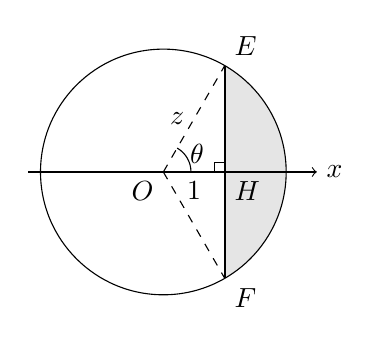
\begin{tikzpicture}[scale=0.78]
                 \fill[gray!20] (1,{-sqrt(3)}) arc[start angle=-60,end angle=60,radius=2] -- cycle;
                 \draw (0,0) circle[radius=2];
                 \draw[thick] (1,{-sqrt(3)}) -- (1,{sqrt(3)});
                 \draw[dashed] (0,0) -- (1,{sqrt(3)}) node[midway,left] {$z$};
                 \draw[dashed] (0,0) -- (1,{-sqrt(3)});
                 \draw[->] (-2.2,0) -- (2.5,0) node[right] {$x$};
                 \draw (0.45,0) arc[start angle=0,end angle=60,radius=0.45];
                 \node at (0.55,0.30) {$\theta$};
                 \node[below left] at (0,0) {$O$};
                 \node[below right] at (1,0) {$H$};
                 \node[above right] at (1,{sqrt(3)}) {$E$};
                 \node[below right] at (1,{-sqrt(3)}) {$F$};
                 \node[below] at (0.5,0) {$1$};
                 \draw (0.84,0) -- (0.84,0.16) -- (1,0.16);
                \end{tikzpicture}
                \end{center}
                図は水平断面で,網掛け部分が求める立体の断面である.
                \,$O$はこの断面の円の中心を表す.
                その面積を$A(z)$とすると,扇形から三角形を引いて,
                \[
                 \begin{aligned}
                 A(z)&=\frac12z^2\cdot2\theta
                      -\frac12\cdot2\sqrt{z^2-1}\cdot1\\
                     &=z^2\theta-\sqrt{z^2-1}.
                 \end{aligned}
                \]
                よって体積は$V=\int_1^2 A(z)\,dz$である.
                \,$z=1/\cos\theta$と置けば,
                \[
                 \sqrt{z^2-1}=\tan\theta,
                 \qquad dz=\frac{\sin\theta}{\cos^2\theta}\,d\theta.
                \]
                したがって,
                \[
                 \begin{aligned}
                 V&=\int_0^{\pi/3}\frac{\theta\sin\theta}{\cos^4\theta}\,d\theta\\
                  &\quad-\int_0^{\pi/3}\frac{\sin^2\theta}{\cos^3\theta}\,d\theta.
                 \end{aligned}
                \]
                第一項では$(\cos^{-3}\theta)'=3\sin\theta/\cos^4\theta$を使って部分積分する.
                第二項では$\sin^2\theta=1-\cos^2\theta$を使うと,
                \[
                 \begin{aligned}
                 V&=\left[\frac{\theta}{3\cos^3\theta}\right]_0^{\pi/3}
                      -\frac13I_3-(I_3-I_1)\\
                  &=\frac{8\pi}{9}-\frac43I_3+I_1\\
                  &=\frac{8\pi}{9}-\frac{4\sqrt3}{3}
                      +\frac13\log(2+\sqrt3).
                 \end{aligned}
                \]
                断面の半径と切断位置の関係を角度で表すと,最初に調べた$I_3$が自然に現れた.
                積分の漸化式は数列だけの技法ではなく,図形から生まれる積分を計算するためにも使える.
          % F6: 一般項を求めずに減衰の速さを決める
          \item 分母に$a_n$があるが,本編の分数型と違って分母が二乗になっている.
                まず逆数を取って,一般項が求められるかだけでなく,増え方を評価できるかを調べる.
                \par\noindent
                \textbf{(1) 逆数の階差を足し合わせる.}
                $a_1=1>0$であり,$a_n>0$なら$(1+2a_n)^2>0$なので$a_{n+1}>0$である.
                よって数学的帰納法からすべての項が正で,$b_n=1/a_n$も定義できる.
                逆数を取ると,
                \[
                 \begin{aligned}
                 b_{n+1}&=\frac{(1+2a_n)^2}{a_n}\\
                         &=b_n+4+4a_n.
                 \end{aligned}
                \]
                したがって$b_{n+1}-b_n=4+4a_n>4$である.
                \,$k=1,\ldots,n-1$について足すと,
                \[
                 b_n-b_1=4(n-1)+4\sum_{k=1}^{n-1}a_k.
                \]
                $b_1=1$より,
                \[
                 b_n=4n-3+4\sum_{k=1}^{n-1}a_k.
                \]
                $n\geq2$なら右辺の総和は正だから,$b_n>4n-3$となる.
                ここまでの変形は,逆数化したあとに階差を総和する本編の技法である.
                ただし総和に$a_k$が残っているため,この式だけでは一般項は得られていない.
                \par\noindent
                \textbf{(2) 項が小さくなることを平均へ移す.}
                正の数の逆数を取ると不等号が逆向きになるので,
                \[
                 0<a_n<\frac1{4n-3}\qquad(n\geq2).
                \]
                挟み撃ちの原理より$a_n\to0$である.
                しかし平均にも$n$が入っているので,項の極限だけで終えず,平均を直接評価する.
                任意の正数$\varepsilon$を取る.
                \,$a_n\to0$より,$k\geq N$なら$0<a_k<\varepsilon$となる正整数$N$が存在する.
                \,$C=\sum_{k=1}^{N-1}a_k$と置けば,$C$は$n$によらない定数である.
                \,$n\geq N$のとき,
                \[
                 \begin{aligned}
                 0<\frac1n\sum_{k=1}^{n}a_k
                 &=\frac Cn+\frac1n\sum_{k=N}^{n}a_k\\
                 &\leq\frac Cn+\frac{n-N+1}{n}\varepsilon\\
                 &\leq\frac Cn+\varepsilon.
                 \end{aligned}
                \]
                十分大きい$n$では$C/n<\varepsilon$でもあるため,平均は$2\varepsilon$より小さい.
                \,$\varepsilon$はいくらでも小さく取れるので,
                \[
                 \lim_{n\to\infty}\frac1n\sum_{k=1}^{n}a_k=0.
                \]
                この証明では,大きかった最初の有限個の項の影響は$n$で割ると消え,
                残りの項はすべて小さい,という二つの点を使っている.
                \par\noindent
                \textbf{(3) 逆数の増え方から元の減衰を読む.}
                (1)の等式を$n$で割ると,
                \[
                 \frac{b_n}{n}=4-\frac3n+
                            \frac4n\sum_{k=1}^{n-1}a_k.
                \]
                (2)より,
                \[
                 0\leq\frac1n\sum_{k=1}^{n-1}a_k
                 \leq\frac1n\sum_{k=1}^{n}a_k\longrightarrow0.
                \]
                したがって$b_n/n\to4$であり,
                \[
                 na_n=\frac1{b_n/n}\longrightarrow\frac14.
                \]
                \par
                最初に求めた上界は,$a_n\to0$を示すための中間結果である.
                それによって階差の追加項$4a_n$の平均が消え,$b_n$は最終的に$4n$と同じ割合で増えると分かった.
                結論$na_n\to1/4$は,$a_n$の減少の速さが$1/(4n)$のそれに近づくことを表す.
                このように,一般項を閉じた式で表さなくても,漸化式から数列の主要な性質を決められる.
          % F7: 1往復で整列できる札の配置
          \item \textbf{(1)~小さい例と, 左端に残る札.}
                $2$枚なら, 昇順の配置はそのまま, 降順の配置は最初の比較で昇順になる.
                よって$c_2=2$である.
                $3$枚では往路の2回の比較で$3$が右端に移る.
                復路では右端の比較は交換を起こさず, 残る2枚が最後の比較で昇順になる.
                したがってすべての配置が成功し,\,$c_3=3!=6$である.
                
                一般に, 最初の比較の直後, 左端の札は
                \[
                  b=\min(A_1,A_2)
                \]
                である. 往路の残りの比較は左端に触れず, 復路でも左端を含む比較は最後に1度だけ行う.
                したがって$b$は最終的に左から1番目か2番目に位置する.
                成功配置ならその数字は$1$または$2$でなければならない.
                これで$\min(A_1,A_2)\le2$が示された.
                ただし, この条件だけで成功が決まるわけではない. 残りの札の並びも調べる必要がある.
                
                \smallskip
                \textbf{(2)~取り除いた札を戻せる対応を作る.}
                比較・交換の結果は, 数字の大小関係だけで決まる.
                そこで札を1枚取り除いた際には, 残りの数字を小さい順に$1,2,\ldots,n-1$と読み替える.
                この読み替えは比較・交換の挙動を変えない.
                
                まず, 成功配置を次の4種類に分ける.
                \[
                \begin{array}{ll}
                \text{\textcircled{1}}&A_1=1,\\
                \text{\textcircled{2}}&A_2=1,\\
                \text{\textcircled{3}}&A_1=2,\ A_2\ge3,\\
                \text{\textcircled{4}}&A_2=2,\ A_1\ge3.
                \end{array}
                \]
                これらは互いに重ならず,\,(1)よりすべての成功配置を尽くす.
                
                \textbf{\textcircled{1},\textcircled{2}の数え方.}
                \textcircled{1}では左端の$1$を取り除く.
                \textcircled{2}では最初の比較によって$1$が左端へ移るので, その$1$を取り除く.
                どちらの場合も, その後の往路は残る$n-1$枚の往路と同じである.
                復路も残る$n-1$枚についての操作を行い, 最後の$1$との比較では交換しない.
                よって元の配置が成功することと, 縮約した配置が成功することは同値である.
                
                逆に,\,$n-1$枚の成功配置の数字をすべて$1$増やし,\,$1$を先頭に挿入すれば\textcircled{1}の配置が得られる.
                $1$を先頭から2番目に挿入すれば\textcircled{2}の配置が得られる.
                いずれも逆操作は一意であるから, 各種類は$c_{n-1}$通りである.
                
                \textbf{\textcircled{3}の数え方.}
                この場合は最初の2枚が$(2,A_2)$で,\,$A_2\ge3$だから最初の比較では交換しない.
                左端の$2$を取り除き, 数字$1$はそのまま,\,$3,4,\ldots,n$をそれぞれ$2,3,\ldots,n-1$に読み替える.
                すると縮約配置の先頭は$1$ではない.
                
                ここで, 元の配置と縮約配置の操作を対応させる.
                元の配置の往路が終わると, 配列は
                \[
                 (2,B_1,B_2,\ldots,B_{n-1})
                \]
                となる. 後ろの$n-1$枚は, 縮約配置の往路後の配列の数字を元に戻したものに等しい.
                復路では, まずこの後ろの$n-1$枚に対し, 縮約問題と同じ比較・交換が行われる.
                
                右から左へ進む1回の操作では, 最小の札$1$は必ずその部分の左端へ移る.
                したがって復路の最後の比較の直前には, 元の配列は
                \[
                 (2,1,D_2,\ldots,D_{n-1})
                \]
                となり, 最後に$(2,1)$が交換される.
                この最終配列が昇順になることは, 縮約問題の最終配列が昇順になることと同値である.
                
                逆に, 先頭が$1$でない$n-1$枚の成功配置で, 数字$2$以上を$1$ずつ増やし,
                先頭に$2$を挿入すれば, 必ず\textcircled{3}の成功配置となる.
                よって求める個数は,\,$n-1$枚の成功配置のうち先頭が$1$でないものの個数である.
                先頭が$1$である成功配置は, 上で示した\textcircled{1}の対応により$c_{n-2}$通りだから,
                \textcircled{3}は$c_{n-1}-c_{n-2}$通りである.
                
                \textbf{\textcircled{4}の数え方.}
                \textcircled{3}の最初の2枚を交換すると,\,$(A_1,2)$で$A_1\ge3$という\textcircled{4}の配置になる.
                最初の比較を済ませれば両者は同じ配列となるので, 成否も一致する.
                この交換は互いに逆だから,\textcircled{4}も$c_{n-1}-c_{n-2}$通りである.
                
                以上を足し合わせると,
                \begin{align*}
                 c_n
                 &=2c_{n-1}+2(c_{n-1}-c_{n-2})\\
                 &=4c_{n-1}-2c_{n-2}\quad(n\ge3).
                \end{align*}
                ここで引いた$c_{n-2}$は, 足し算で生じた曖昧な重複ではなく,
                \textcircled{3}の縮約先から除かなければならない「先頭が$1$の配置」の数である.
                
                \smallskip
                \textbf{(3)~数える問題から, 3項間漸化式へ.}
                特性方程式は
                \[
                 x^2-4x+2=0
                \]
                であり, 根は$2+\sqrt2,2-\sqrt2$である.
                したがって定数$P,Q$を用いて
                \[
                 c_n=P(2+\sqrt2)^{n-1}+Q(2-\sqrt2)^{n-1}
                \]
                と書ける. $c_1=1,c_2=2$より
                \[
                 P+Q=1,\qquad
                 (2+\sqrt2)P+(2-\sqrt2)Q=2.
                \]
                これを解くと$P=Q=1/2$なので,
                \[
                 c_n=\frac{(2+\sqrt2)^{n-1}+(2-\sqrt2)^{n-1}}2.
                \]
                例えば$c_4=20,c_5=68$となる.
                無理数を含む式で配置の個数という整数が表されるのは,
                2つのべきの展開に現れる$\sqrt2$の奇数次の項が相殺されるためである.
                この問題では, 本編の解法を使うまでの「何を数え, 何を取り除くか」の設計が中心である.
          % F8: 巨大な項の整除と, 添字の互除法
          \item \textbf{(1)~余りも漸化式に従う.}
                この数列の最初の項は
                \[
                 1,2,5,26,677,\ldots
                \]
                であり, 値を直接計算して調べ続ける方法はすぐに難しくなる.
                一方,\,$a_n$を$5$で割った余りが$r$なら,
                $a_{n+1}$の余りは$r^2+1$を$5$で割った余りである.
                そこで余りだけを調べると,
                \[
                 1\longmapsto2\longmapsto0\longmapsto1
                \]
                となる. 同じ余りに戻れば, それ以後の余りも同じ規則で繰り返される.
                したがって
                \[
                 a_n\equiv
                 \begin{cases}
                 1 & (n\equiv1\pmod3),\\
                 2 & (n\equiv2\pmod3),\\
                 0 & (n\equiv0\pmod3)
                 \end{cases}
                 \quad(\bmod5).
                \]
                よって$a_n$が$5$の倍数となるのは,\,$n$が$3$の正の倍数であるときに限る.
                
                \smallskip
                \textbf{(2)~法を数列の項にする.}
                補助的に$a_0=0$と定める.
                すると$a_1=a_0^2+1$も成り立つので, 漸化式は$n\ge0$で使える.
                任意の正整数$m$を固定し,
                \[
                 a_{m+j}\equiv a_j\pmod{a_m}
                 \quad(j\ge0)
                \]
                を示そう.
                $j=0$では両辺が$0$と合同である.
                $j$で成り立つと仮定すると,
                \begin{align*}
                 a_{m+j+1}
                 &=a_{m+j}^2+1\\
                 &\equiv a_j^2+1=a_{j+1}\pmod{a_m}.
                \end{align*}
                よって数学的帰納法により, すべての$j\ge0$で成り立つ.
                
                ここで$n=qm+r\ (0\le r<m)$と割り算すると,
                上の合同式を繰り返し使うことで
                \[
                 a_n\equiv a_r\pmod{a_m}
                \]
                が得られる.
                さらに$a_0=0,a_1=1$であり,\,$n\ge1$では
                \[
                 a_{n+1}-a_n=a_n(a_n-1)+1>0
                \]
                だから, 数列は$a_0$から厳密に増加する.
                したがって$0\le r<m$に対して
                \[
                 0\le a_r<a_m,
                \]
                しかも$a_r=0$となるのは$r=0$のときだけである.
                よって
                \begin{align*}
                 a_m\mid a_n
                 &\Longleftrightarrow a_r=0\\
                 &\Longleftrightarrow r=0\\
                 &\Longleftrightarrow m\mid n.
                \end{align*}
                この議論は$m=1$でも成り立つ. このとき余りの添字は必ず$r=0$で,
                $a_1=1$はすべての整数を割り切る.
                なお,\,$a_3=5$であるから,\,(1)はこの結果の$m=3$という特別な場合でもある.
                
                \smallskip
                \textbf{(3)~項の互除法を, 添字の互除法へ移す.}
                再び$n=qm+r\ (0\le r<m)$とおく.
                $a_n\equiv a_r\pmod{a_m}$であるから,\,$a_n$と$a_r$の差は$a_m$の整数倍である.
                よって$a_m$と$a_n$の共通の約数は,\,$a_m$と$a_r$の共通の約数に一致する.
                したがって
                \[
                 \gcd(a_m,a_n)=\gcd(a_m,a_r).
                \]
                これは, 添字に対して行うユークリッドの互除法に沿って,
                項の最大公約数を保ったまま添字を小さくできることを意味する.
                添字の互除法は,\,$d=\gcd(m,n)$と$0$で終わるので,
                \[
                 \gcd(a_m,a_n)=\gcd(a_d,a_0)=a_d.
                \]
                最後の等号は,\,$a_0=0$であり,\,$\gcd(x,0)=x$だからである.
                
                求める例では,
                \begin{align*}
                 3040&=2026+1014,\\
                 2026&=1014+1012,\\
                 1014&=1012+2,\\
                 1012&=506\cdot2
                \end{align*}
                だから,\,$\gcd(2026,3040)=2$である.
                従って
                \[
                 \gcd(a_{2026},a_{3040})=a_2=2.
                \]
                項がどれほど大きくなっても, 添字の小さな整数計算だけでこの最大公約数が決まる.
                漸化式は項の値を求めるだけでなく, 整除のような「項どうしの関係」を取り出す道具にもなる.
          % F9: 整数方程式の解を生み出す漸化式
          \item \textbf{(1)~1つの解から次の解へ.}
                $x=3$のとき, 方程式は
                \[
                 9+y^2+z^2=3yz
                \]
                となる. $z$を固定して$y$の2次方程式とみれば,
                もう1つの根は$3z-y$であることが, 根と係数の関係から予想できる.
                実際に確かめると,
                \begin{align*}
                 &9+z^2+(3z-y)^2-3z(3z-y)\\
                 &\qquad=9+y^2+z^2-3yz=0.
                \end{align*}
                よって$(3,z,3z-y)$も方程式を満たす.
                しかも$3z-y$は整数であり,\,$0<y\le z$より
                \[
                 3z-y\ge2z>z>0.
                \]
                したがって正の整数解である.
                この操作で新しくできた2つの数も$z<3z-y$を満たすため, 同じ操作を繰り返せる.
                
                \smallskip
                \textbf{(2)~解を作る操作を数列にする.}
                最初の解$(3,3,3)$から(1)の操作を繰り返すと,\,$y,z$は
                \[
                 (3,3),\ (3,6),\ (6,15),\ (15,39),\ldots
                \]
                と変化する.
                この隣接する2つの数を$u_n,u_{n+1}$とすれば, 次の数は$3u_{n+1}-u_n$となる.
                これが問題で与えた3項間漸化式の意味である.
                
                特性方程式は
                \[
                 t^2-3t+1=0
                \]
                であり, 2つの根を
                \[
                 \alpha=\frac{3+\sqrt5}2,\qquad
                 \beta=\frac{3-\sqrt5}2
                \]
                とおく.
                $u_n=P\alpha^n+Q\beta^n$と書くと,\,$u_0=u_1=3$より
                \[
                 P+Q=3,\qquad \alpha P+\beta Q=3.
                \]
                これを解けば
                \[
                 P=\frac{3(\sqrt5-1)}{2\sqrt5},\qquad
                 Q=\frac{3(\sqrt5+1)}{2\sqrt5}.
                \]
                したがって
                \begin{align*}
                 u_n
                 &=P\alpha^n+Q\beta^n\\
                 &=\frac32\left\{\alpha^n+\beta^n
                 -\frac{\alpha^n-\beta^n}{\sqrt5}\right\}.
                \end{align*}
                
                \smallskip
                \textbf{(3)~一般項とは別に, 整数性と方程式を保証する.}
                初期値は整数であり, 漸化式は整数の3倍と整数の差で次の項を作る.
                したがって数学的帰納法により, すべての$u_n$は整数である.
                また$u_0=u_1=3>0,u_2=6>u_1$である.
                $u_{n+1}>u_n>0$なら
                \[
                 u_{n+2}=3u_{n+1}-u_n>2u_{n+1}>u_{n+1}
                \]
                だから,\,$n\ge1$で$u_{n+1}>u_n>0$が成り立つ.
                
                さらに, 隣接する2項から作る量
                \[
                 I_n=u_n^2+u_{n+1}^2-3u_nu_{n+1}
                \]
                を考える.
                漸化式を代入すると,
                \begin{align*}
                 I_{n+1}
                 &=u_{n+1}^2+(3u_{n+1}-u_n)^2\\
                 &\quad{}-3u_{n+1}(3u_{n+1}-u_n)\\
                 &=u_n^2+u_{n+1}^2-3u_nu_{n+1}=I_n.
                \end{align*}
                従ってこの量は変わらず,
                \[
                 I_n=I_0=9+9-27=-9.
                \]
                よって
                \[
                 3^2+u_n^2+u_{n+1}^2=3u_nu_{n+1}.
                \]
                以上から$(3,u_n,u_{n+1})$は正の整数解である.
                $n\ge1$で$u_{n+1}$が厳密に増加するので, これらの三つ組は互いに異なり, 解は無限個ある.
                ここでは特定の操作で得られる解の系列を作っており, すべての解の分類までは要求していない.
                
                最後に比の極限を求める.
                $0<\beta<1<\alpha$であり,\,$P,Q>0$だから,
                \[
                 \frac{u_{n+1}}{u_n}
                 =\alpha\,
                 \frac{P+Q(\beta/\alpha)^{n+1}}
                      {P+Q(\beta/\alpha)^n}
                 \longrightarrow\alpha.
                \]
                一般項には無理数が現れるが, 漸化式が整数性を保証する.
                さらに整数どうしの比が無理数$\alpha$へ近づくことまで分かる.
                解法としての3項間漸化式が, 整数解を無限に生成する仕組みと, その増加の速さを同時に記述している.
          % F10: 元のペアをすべて解消する組み替え
          \item \textbf{(1) 小さい場合で数える対象を確認する.}
                $n=1$では組み替える相手がいないため,\,$S(1)=0$である.
                $n=2$では$(A_1,B_2),(A_2,B_1)$の1通りである.
                $n=3$では,\,$A_1,A_2,A_3$の相手の添字が
                $(2,3,1)$または$(3,1,2)$となる2通りなので,\,$S(3)=2$である.
                $S(0)=1$は, 要素がない場合の「何も作らない組合せ」を1通りと数える約束である.
                \par\smallskip
                \textbf{(2) 相手を1個決め, 残りを小さい問題に戻す.}
                $A_1$の相手$B_j$は,\,$j\ne1$の$n-1$通りから選ぶ.
                以後は$j$を固定する.
                \par
                まず$A_j$の相手が$B_1$なら,\,$A_1,A_j,B_1,B_j$を除いた残りの$n-2$組を,
                元のペアが残らないように作ればよい.
                これは$S(n-2)$通りである.
                \par
                次に$A_j$の相手が$B_1$でないとする.
                $B_1$の相手を$A_k$とすると,\,$k\ne1,j$である.
                2組のペア
                \[
                 (A_1,B_j),\quad(A_k,B_1)
                \]
                から$A_1,B_1$を除き,\,$(A_k,B_j)$の1組に置き換える.
                $k\ne j$なので, この新しいペアも元のペアではない.
                したがって, 添字$2,\ldots,n$の$n-1$組を完全に組み替えた形になる.
                \par
                逆に, そのような$n-1$組の組合せから$B_j$の相手$A_k$を見つけ,
                \[
                 (A_k,B_j)\ \longmapsto
                 (A_1,B_j),(A_k,B_1)
                \]
                と戻せば, 元の組合せが一意に復元できる.
                つまり, 対応は一対一であり, 後者は$S(n-1)$通りである.
                この「小さくした問題に戻せること」が, 個数の漸化式を作る根拠である.
                2つの場合は重ならないので,
                \[
                 S(n)=(n-1)\{S(n-1)+S(n-2)\}.
                \]
                \par\smallskip
                \textbf{(3) 変動する係数を, 差と階乗で整理する.}
                この漸化式は係数が$n$に依存するため, 定数係数の3項間漸化式としては解けない.
                そこで
                \[
                 T_n=S(n)-nS(n-1)\quad(n\ge1)
                \]
                とおく. $n\ge2$では(2)から
                \begin{align*}
                 T_n
                 &= (n-1)S(n-2)-S(n-1)\\
                 &= -T_{n-1}.
                \end{align*}
                $T_1=S(1)-S(0)=-1$より,\,$T_n=(-1)^n$である.
                よって
                \[
                 S(n)=nS(n-1)+(-1)^n.
                \]
                ここで$n$を階比として吸収するため,\,$P_n=S(n)/n!$とおく.
                \[
                 P_n-P_{n-1}=\frac{(-1)^n}{n!}.
                \]
                $P_0=S(0)/0!=1$より, 階差を足し合わせると
                \[
                 P_n=\sum_{k=0}^{n}\frac{(-1)^k}{k!}.
                \]
                したがって,
                \[
                 S(n)=n!\sum_{k=0}^{n}\frac{(-1)^k}{k!}.
                \]
                なお,\,$S(4)=9,\,S(5)=44$もこの式や(2)から求められる.
                本編の\textbf{等比型, 階比による正規化, 階差型}を順に使ったことになる.
                \par\smallskip
                \textbf{(4) 残る組数を指定して数える.}
                元のペアをちょうど$r$組残すには, まず残す$r$組を$\binom{n}{r}$通りから選ぶ.
                残りの$n-r$組では元のペアを1組も残せないので, その組み方は$S(n-r)$通りである.
                どの$r$組が残るかは完成形から一意に決まるため, 重複はない.
                よって答えは
                \[
                 \binom{n}{r}S(n-r)
                \]
                である. $r=n$でも$S(0)=1$によって1通りと数えられる.
                \par
                次に, 全組合せで残る元のペアの組数を合計する.
                固定したペア$(A_i,B_i)$が残る組合せは, 残りの相手を自由に割り当てる$(n-1)!$通りである.
                これを$i=1,\ldots,n$について足すと, 合計は$n(n-1)!$となる.
                元のペアが$r$組残る組合せはちょうど$r$回数えられるので, この合計でよい.
                全組合せは$n!$通りであるから, 平均値は$n(n-1)!/n!=1$である.
                \par\smallskip
                \noindent\textbf{【数学的な広がり：完全順列と確率】}\par\nopagebreak[4]
                元の位置に戻る要素のない並べ替えを\textbf{完全順列（錯置）}と呼ぶ.
                この問題はその数え上げである.
                また, 全$n!$通りを同じ確率で選ぶとき, 元のペアが1組も残らない確率は
                \[
                 P_n=\frac{S(n)}{n!}
                     =\sum_{k=0}^{n}\frac{(-1)^k}{k!}
                \]
                である. このように,\,$n!$で割る操作には, 漸化式を整理するだけでなく\textbf{個数を確率に直す意味}もある.
                \par
                さらに, この確率は$n$が大きくなると$1/e$に近づく.
                ここでは無限級数展開を仮定せず, 本編の二項定理と$e$の定義で確認しよう.
                \par
                まず$m\ge0$について,
                \begin{align*}
                 P_{2m+2}-P_{2m}
                 &= -\frac{2m+1}{(2m+2)!}<0,\\
                 P_{2m+3}-P_{2m+1}
                 &= \frac{2m+2}{(2m+3)!}>0.
                \end{align*}
                また,\,$P_{2m}-P_{2m+1}=1/(2m+1)!$である.
                したがって, 偶数番目の確率は減少し, 奇数番目の確率は増加し, 両者の差は0へ近づく.
                確率は$0$以上$1$以下なので, それぞれ収束し, 共通の極限$L$をもつ.
                \par
                その値を決めるため, 整数$M\ge2$に対して
                \[
                 b_{M,k}=\frac{\binom{M}{k}}{M^k}
                 \quad(0\le k\le M)
                \]
                とおく. すると
                \[
                 \frac{b_{M,k+1}}{b_{M,k}}
                 =\frac{M-k}{M(k+1)}\le1
                \]
                なので,\,$b_{M,k}$は$k$について非増加である.
                二項定理の有限和を,添字$k$が偶数または奇数の項で止める.
                残りを隣り合う2項ずつ組にすることで,
                $M\ge2\ell+1$に対して
                \begin{align*}
                 \sum_{k=0}^{2\ell+1}(-1)^k b_{M,k}
                 &\le\left(1-\frac1M\right)^M,\\
                 \left(1-\frac1M\right)^M
                 &\le\sum_{k=0}^{2\ell}(-1)^k b_{M,k}
                \end{align*}
                が分かる. 添字が奇数の項で止めた残りは「正の項$-$次の項」の和となり0以上で,
                添字が偶数の項で止めた残りはその符号が逆になる.
                \par
                ここで$\ell$を固定し,\,$M\to\infty$とする.
                固定した$k$について
                \[
                 b_{M,k}=\frac1{k!}
                 \prod_{j=0}^{k-1}\left(1-\frac jM\right)
                 \longrightarrow\frac1{k!}.
                \]
                $k=0$の積は$1$とする.
                一方,\,$t=M-1$とおくと,
                \[
                 \left(1-\frac1M\right)^M
                 =\left(1+\frac1t\right)^{-t-1}.
                \]
                本編の$e$の定義から,$(1+1/t)^t\to e$であり,
                $(1+1/t)\to1$なので,上の式は$1/e$へ近づく.
                よって
                \[
                 P_{2\ell+1}\le\frac1e\le P_{2\ell}.
                \]
                今度は$\ell\to\infty$とし, 挟み撃ちによって$L=1/e$を得る.
                \[
                 \boxed{\lim_{n\to\infty}\frac{S(n)}{n!}
                       =\frac1e\simeq0.368}.
                \]
                同じ偶奇の後の項は極限へ向かって厳密に進むため,
                $1/e$は隣り合う$P_n,P_{n+1}$の間に厳密に入る. よって$n\ge1$で
                \begin{align*}
                 \left|P_n-\frac1e\right|
                 &<\frac1{(n+1)!},\\
                 \left|S(n)-\frac{n!}{e}\right|
                 &<\frac1{n+1}\le\frac12.
                \end{align*}
                下段は上段を$n!$倍して得られる.
                つまり,\,$S(n)$は$n!/e$に最も近い整数である.
                場合の数を数える漸化式から, 階乗, 確率, 自然対数の底が一つにつながった.
        \end{enumerate}



\end{bookcolumns}
